\chapter{Results}
\label{cha:results}

\section{Continuum kernel on \(S^1\)}

We first state the explicit form of the limiting neural tangent kernel on the circle and the
corresponding Fourier eigenvalues of the integral operator \(T\) introduced in
Chapter~\ref{cha:methodology}. The calculation uses the standard infinite-width NTK
description of \citet{jacot2018ntk}, together with the
arc-cosine formulas for ReLU Gaussian averages \citep{cho2009kernel}. Related spectral
calculations for ReLU NTKs on the sphere appear in
\citet{basri2019convergence,bietti2019inductivebiasneuraltangent,cao2020understandingspectralbiasdeep}. The derivation in the
assumptions used here is given in Appendix~\ref{app:continuum-kernel}.

\begin{proposition}[Limiting NTK on \(S^1\)]
	\label{prop:results-continuum-ntk}
	Consider the finite-width network \(f_m\) and initialization from
	\eqref{eq:method-network-model}--\eqref{eq:method-network-initialization}.
	For \(x(\varphi)=(\cos\varphi,\sin\varphi)\), define the finite-width NTK at
	initialization by
	\[
		\Theta_m(\varphi,\psi)
		=
		\left\langle
		\nabla_\theta f_m(x(\varphi);\theta_0),
		\nabla_\theta f_m(x(\psi);\theta_0)
		\right\rangle .
	\]
	The limiting NTK is the deterministic kernel
	\[
		\Theta(\varphi,\psi)
		=
		\lim_{m\to\infty}\Theta_m(\varphi,\psi),
	\]
	where the limit is taken pointwise over the random initialization.

	If \(\delta=d(\varphi,\psi)\in[0,\pi]\) denotes the angular distance
	between \(x(\varphi)\) and \(x(\psi)\), then \(\Theta(\varphi,\psi)\) depends
	only on \(\delta\) and is given by
	\begin{equation}
		\Theta(\delta)
		=
		\frac{1}{2\pi}
		\Bigl(
		\sin\delta + 2(\pi-\delta)\cos\delta + (\pi-\delta)
		\Bigr).
		\label{eq:results-continuum-ntk}
	\end{equation}
	Extending \(\Theta(\delta)\) to an even \(2\pi\)-periodic function, the
	associated integral operator is
	\begin{equation}
		(Tf)(\varphi)
		=
		\int_0^{2\pi}\Theta(\varphi-\psi)f(\psi)\,d\mu(\psi).
		\label{eq:results-continuum-operator}
	\end{equation}
\end{proposition}

Since \(T\) is a convolution operator, it is diagonalized by the real Fourier basis
introduced in \eqref{eq:method-fourier-basis-phi0}--\eqref{eq:method-fourier-basis-modes}.

\begin{theorem}[Fourier eigenvalues of the limiting NTK]
	\label{thm:results-continuum-spectrum}
	Let \(\lambda_k\) denote the eigenvalue of \(T\) corresponding to the
	Fourier frequency \(k\) introduced in
	\eqref{eq:method-fourier-basis-phi0}--\eqref{eq:method-fourier-basis-modes}.
	Then
	\begin{equation}
		\lambda_0=\frac{1}{4}+\frac{3}{\pi^2},
		\qquad
		\lambda_1=\frac{1}{4}+\frac{1}{\pi^2},
		\label{eq:results-lambda-0-1}
	\end{equation}
	and for \(k\geq 2\),
	\begin{equation}
		\lambda_k=
		\begin{cases}
			\dfrac{k^2+3}{\pi^2(k^2-1)^2}, & k \ge 2 \text{ even}, \\[1em]
			\dfrac{1}{\pi^2 k^2},          & k \ge 3 \text{ odd}.
		\end{cases}
		\label{eq:results-lambda-k}
	\end{equation}
	In particular, the decay rates of the Fourier components of the residual are determined by
	these eigenvalues.
\end{theorem}

The detailed derivation is provided in Appendix~\ref{sec:app-fourier-coefficients}.

The eigenvalues decrease with frequency. Both even and odd modes satisfy
\(\lambda_k=O(k^{-2})\) for large \(k\), so higher-frequency residual
components decay more slowly under fixed-kernel gradient flow. This gives the
continuum spectral-bias baseline used in the rest of the chapter.

\begin{corollary}[Spectrum without the trainable bias]
	\label{cor:results-bias-spectrum}
	Let \(\Theta^{(\mathrm{nb})}\) denote the limiting NTK obtained by removing the
	trainable hidden-bias contribution, while keeping the output-weight and input-weight
	contributions. Then, on \(S^1\),
	\begin{equation}
		\Theta^{(\mathrm{nb})}(\delta)
		=
		\frac{1}{2\pi}
		\Bigl(
		\sin\delta+2(\pi-\delta)\cos\delta
		\Bigr).
		\label{eq:results-no-bias-kernel}
	\end{equation}
	Let \(\lambda_k^{(\mathrm{nb})}\) denote the corresponding Fourier eigenvalue. Then
	\begin{equation}
		\lambda_0^{(\mathrm{nb})}=\frac{3}{\pi^2},
		\qquad
		\lambda_1^{(\mathrm{nb})}=\frac14,
		\label{eq:results-no-bias-lambda-0-1}
	\end{equation}
	and, for \(k\ge 2\),
	\begin{equation}
		\lambda_k^{(\mathrm{nb})}
		=
		\begin{cases}
			\dfrac{k^2+3}{\pi^2(k^2-1)^2}, & k\ge 2 \text{ even}, \\[1em]
			0,                             & k\ge 3 \text{ odd}.
		\end{cases}
		\label{eq:results-no-bias-lambda-k}
	\end{equation}
	Consequently, comparing with Theorem~\ref{thm:results-continuum-spectrum}, the
	trainable bias leaves the even frequencies \(k\ge 2\) unchanged, increases the constant
	and \(k=1\) eigenvalues, and supplies the nonzero eigenvalues of all odd modes
	\(k\ge 3\). Thus the odd modes \(k\ge 3\) are absent from the no-bias fixed-kernel
	dynamics but present in the model studied here.
\end{corollary}

The detailed derivation is provided in Appendix~\ref{sec:app-bias-contribution}.

The trainable hidden bias affects the nullspace of the continuum operator.
Corollary~\ref{cor:results-bias-spectrum} shows that, without the bias
contribution, the odd modes \(k\ge 3\) have zero eigenvalue. With the bias
contribution, these modes acquire nonzero but small eigenvalues. Thus, the bias
determines whether these modes can be learned in the fixed-kernel continuum
dynamics. This is consistent with earlier harmonic analyses of two-layer ReLU networks on
the sphere and circle, where bias-free two-layer models do not express odd
harmonics beyond the first frequency
\citep{basri2019convergence,basri2020frequencybiasneuralnetworks}.

\subsection{Continuum fixed-kernel dynamics}
\label{subsec:results-continuum-fixed-kernel-dynamics}

The eigenvalues in Theorem~\ref{thm:results-continuum-spectrum} determine the
ideal fixed-kernel dynamics. Write the residual from
Section~\ref{subsec:least-squares-loss-and-residual-dynamics} in the real
Fourier basis as
\[
	r_t=\sum_p \alpha_p(t)\phi_p .
\]
Here, \(\alpha_p\) is the amplitude associated with mode \(p\), \(\lambda_p\)
denotes the eigenvalue associated with the Fourier frequency of \(\phi_p\) and
\(\Lambda=\operatorname{diag}(\lambda_p)\).
Since \(T\phi_p=\lambda_p\phi_p\), gradient flow gives
\begin{equation}
	\alpha_p(t)
	=
	\exp(-\lambda_p t)\alpha_p(0).
	\label{eq:results-continuum-gradient-flow-mode-decay}
\end{equation}
Thus the normalized amplitude \(|\alpha_p(t)|/|\alpha_p(0)|\) is set by the
eigenvalue of the corresponding Fourier mode.

Figure~\ref{fig:results-continuum-spectral-bias-first200} shows this diagonal
continuum dynamics for the kernel with and without the trainable-bias
contribution. Low-frequency components decay faster than high-frequency
components.

\begin{figure}[!htbp]
	\centering
	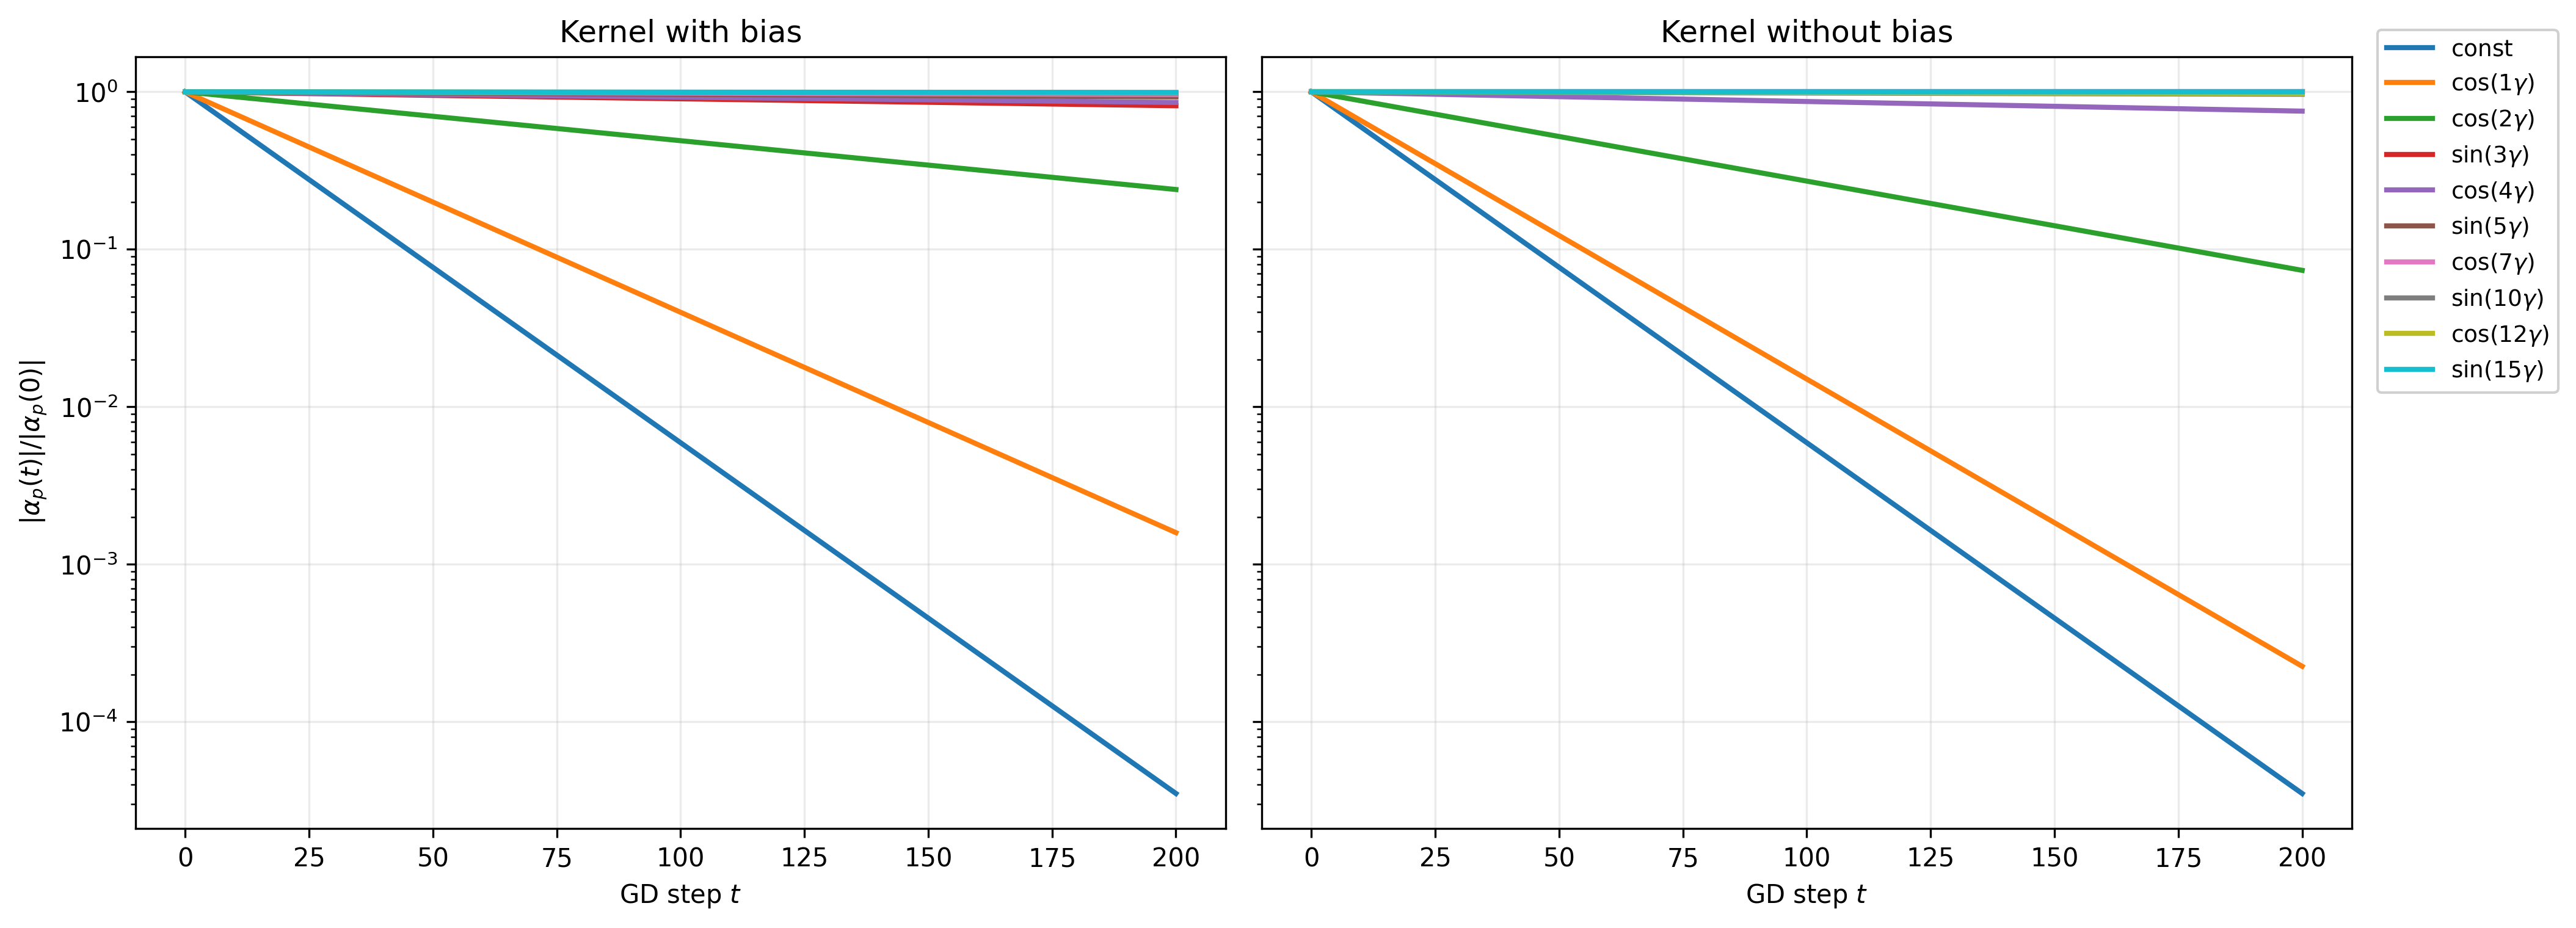
\includegraphics[width=\textwidth]{images/finite_sample_results/story_01_spectral_bias_two_panel_first200.png}
	\caption{Continuum fixed-kernel dynamics for the first \(200\) gradient
		descent steps, comparing the kernel with and without the trainable-bias
		contribution. The curves show normalized mode amplitudes of the residual
		\(|\alpha_p(t)|/|\alpha_p(0)|\) under the diagonal Fourier dynamics.}
	\label{fig:results-continuum-spectral-bias-first200}
\end{figure}

Figure~\ref{fig:results-continuum-odd-modes} isolates odd Fourier modes. With the bias contribution, these modes have nonzero eigenvalues. Without the
bias contribution, the plotted odd modes have zero eigenvalues and remain
constant under the fixed-kernel dynamics.

\begin{figure}[!htbp]
	\centering
	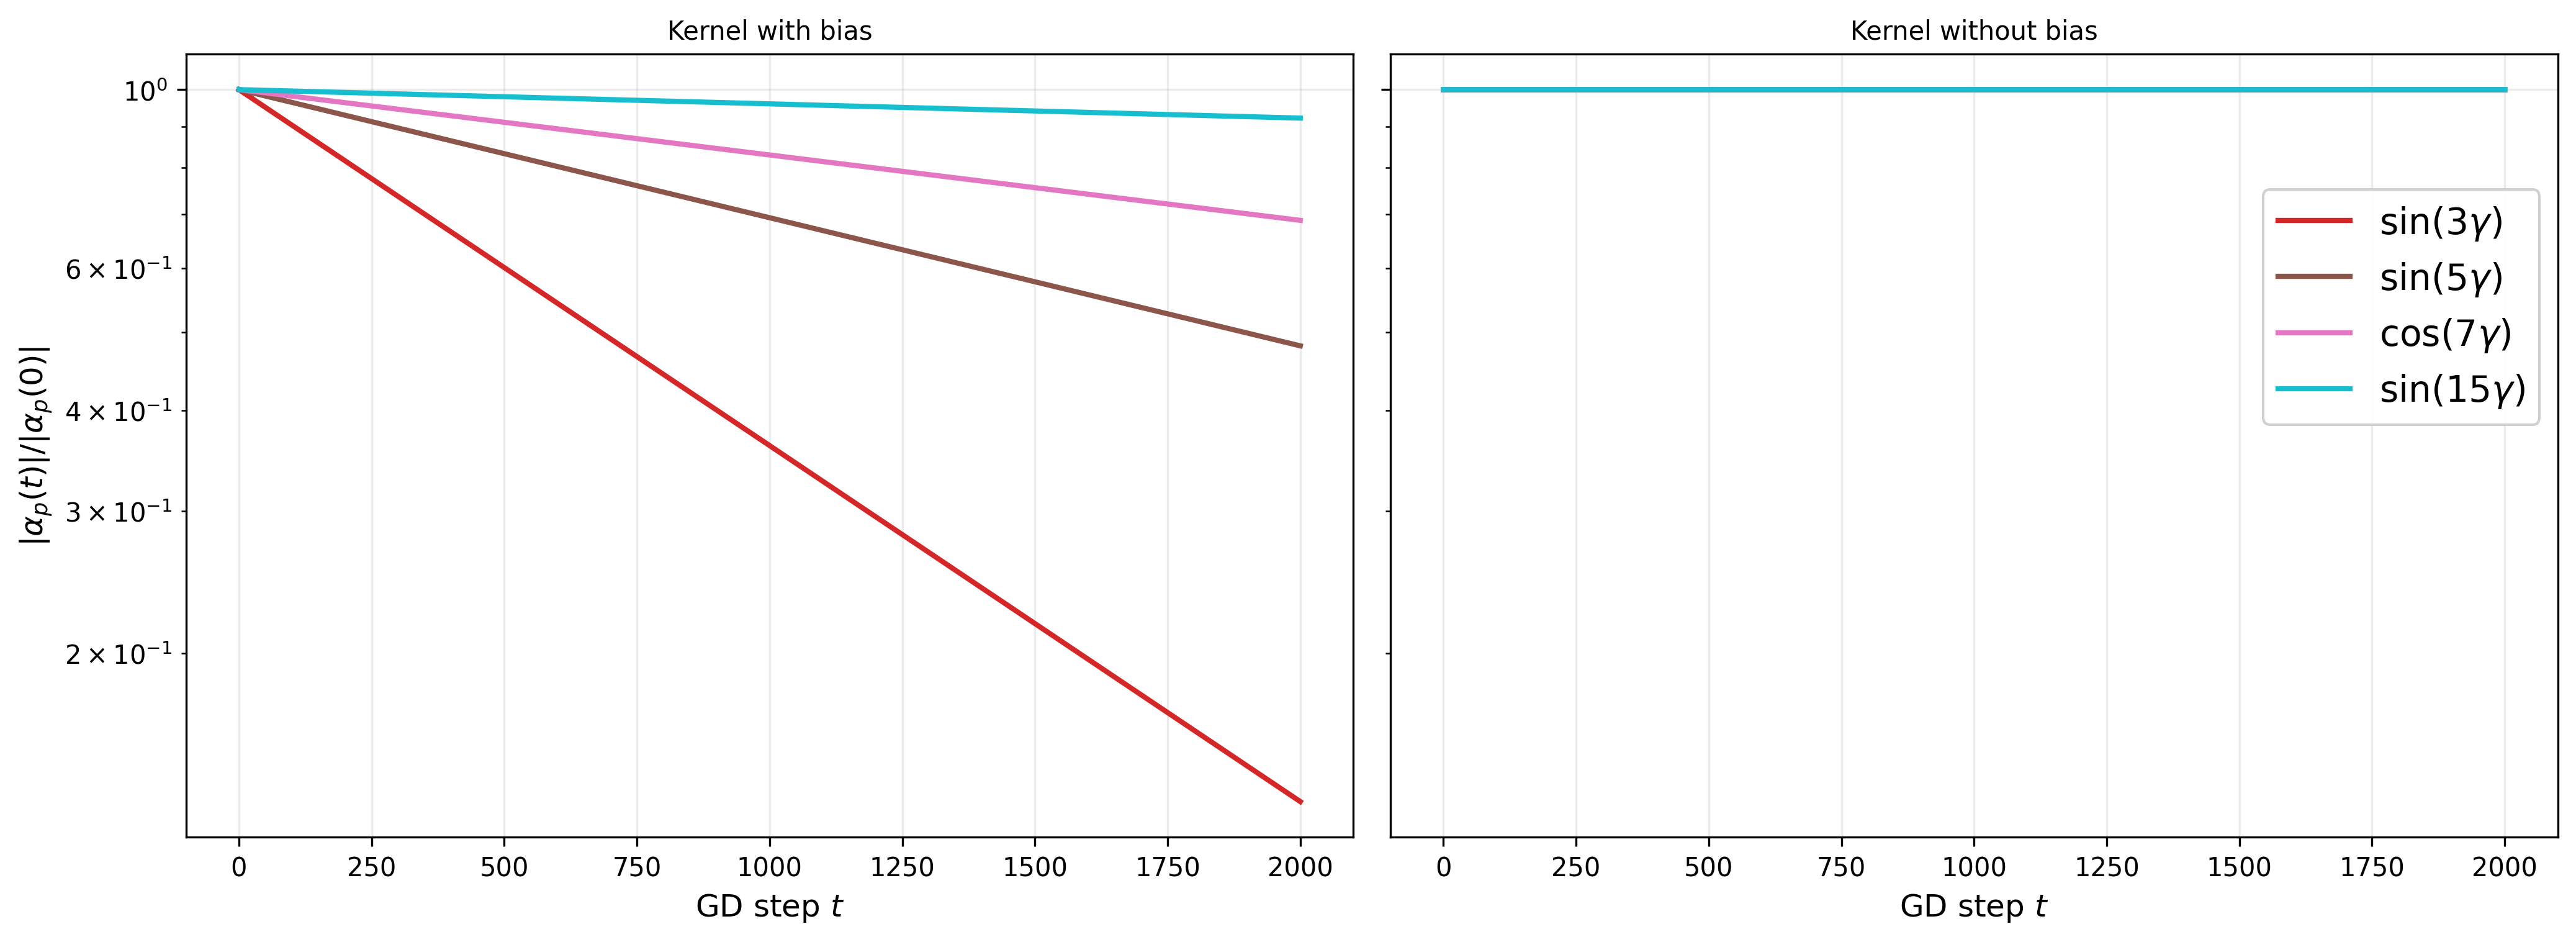
\includegraphics[width=\textwidth]{images/finite_sample_results/story_01_spectral_bias_two_panel_high_freq_odd.png}
	\caption{Odd-mode continuum fixed-kernel dynamics with and without the
		trainable-bias contribution. With the bias contribution, the plotted odd modes
		have nonzero eigenvalues. Without it, the plotted odd modes have zero
		eigenvalues and therefore remain constant under the fixed-kernel dynamics.}
	\label{fig:results-continuum-odd-modes}
\end{figure}

Together, these calculations and plots give the continuum reference case. Here
the operator is the deterministic infinite-width integral operator \(T\), defined
using the uniform measure on \(S^1\). Thus the Fourier frequency subspaces are
exact invariant subspaces of the dynamics, and each residual component decays at
the rate given by the corresponding eigenvalue. This is the standard NTK
spectral mechanism in an explicit setting. Components aligned with larger kernel
eigenvalues decay faster
\citep{jacot2018ntk,lee2020wide,cao2020understandingspectralbiasdeep}. Because
the domain and measure are rotationally symmetric, this eigenvalue ordering is
also a frequency ordering
\citep{bietti2019inductivebiasneuraltangent,basri2019convergence,
	basri2020frequencybiasneuralnetworks}.

With this continuum baseline in place, we now ask how much of this Fourier
structure survives after replacing the uniform measure by finitely many sampled
points.

\section{Finite-sample control on a truncated Fourier subspace}
\label{sec:results-finite-sample}

We now turn to the sampled setting introduced in
section~\ref{sec:finite-sample-methodology}. Throughout, \(K\geq 1\) is fixed,
\(d=2K+1\), and the truncated Fourier subspace \(\mathcal H_K\) is given by
\eqref{eq:method-low-frequency-subspace}. Recall from
Section~\ref{subsec:real-fourier-basis-truncates-subspaces} that, for a basis
function in \(\mathcal H_K\), its frequency means its Fourier index. Thus
\(\phi_0\) has frequency \(0\), corresponding to the constant mode, while both
\(\phi_{k,c}\) and \(\phi_{k,s}\) have frequency \(k\). The matrices
\(\Phi\), \(A\), \(G\), and \(H\) are defined in
\eqref{eq:method-feature-matrix}--\eqref{eq:method-compressed-operator}.

For each basis index \(p\), let \(k(p)\) denote the frequency of the corresponding basis
function \(\phi_p\), and write
\[
	\lambda_p:=\lambda_{k(p)}.
\]

\begin{proposition}[Expectation of the restricted sampled operator]
	\label{prop:results-expectation-H}
	Define
	\begin{equation}
		\lambda_p^{(n)}
		=
		\left(1-\frac{1}{n}\right)\lambda_p+\frac{\Theta(0)}{n},
		\label{eq:results-finite-sample-corrected-eigs}
	\end{equation}
	and let
	\begin{equation}
		\Lambda^{(n)}=\operatorname{diag}(\lambda_p^{(n)}).
		\label{eq:results-finite-sample-eigenvalue-matrix}
	\end{equation}
	Then
	\begin{equation}
		\mathbb E[H]=\Lambda^{(n)}.
		\label{eq:results-expected-H}
	\end{equation}
\end{proposition}

The detailed proof is provided in Appendix~\ref{sec:app-expected-H}.

The finite-sample eigenvalue \(\lambda_p^{(n)}\) differs from the continuum
value \(\lambda_p\) by a term of order \(\frac{\Theta(0)}{n}\). This correction
shrinks with \(n\), so the sampled eigenvalues approach the continuum values as
the sample size grows. For the kernel values and block dimensions used in the
experiments, this correction is small once \(n\) is a few hundred.

The next theorem gives explicit concentration bounds for the three sampled quantities that
appear in the methodology chapter.

\begin{theorem}[Finite-sample concentration on the truncated Fourier subspace]
	\label{thm:results-finite-sample-concentration}
	Assume that
	\begin{equation}
		\kappa:=\sup_{\theta\in[0,2\pi)}|\Theta(\theta)|<\infty.
		\label{eq:results-kappa}
	\end{equation}
	Then, for every \(\varepsilon>0\),
	\begin{equation}
		\mathbb P\!\left(\|G-I_d\|_{\max}\ge \varepsilon\right)
		\le
		d(d+1)\exp\!\left(-\frac{n\varepsilon^2}{4+\frac43\varepsilon}\right),
		\label{eq:results-gram-concentration}
	\end{equation}
	\begin{equation}
		\mathbb P\!\left(\|H-\Lambda^{(n)}\|_{\max}\ge \varepsilon\right)
		\le
		2d^2\exp\!\left(-\frac{n\varepsilon^2}{32\kappa^2}\right),
		\label{eq:results-H-concentration}
	\end{equation}
	and, for \(n\ge 2\),
	\begin{equation}
		\mathbb P\!\left(\|A\Phi-\Phi\Lambda^{(n)}\|_{\max}\ge \varepsilon\right)
		\le
		2nd\exp\!\left(-\frac{n\varepsilon^2}{2\kappa^2+2\kappa\varepsilon}\right).
		\label{eq:results-APhi-concentration}
	\end{equation}
\end{theorem}

The detailed proofs of the three bounds are provided in
Appendix~\ref{app:finite-sample-proofs}.

Combining the preceding concentration bounds gives a single high-probability
event on which all three finite-sample quantities are controlled at once.
Namely, with probability at least \(1-\delta\),
\[
	\|G-I_d\|_{\max},
	\qquad
	\|H-\Lambda^{(n)}\|_{\max},
	\qquad
	\|A\Phi-\Phi\Lambda^{(n)}\|_{\max}
\]
are all of order
\[
	O \left(  \sqrt{\frac{\log(nd/\delta)}{n}}\right) ,
\]
up to logarithmic-over-\(n\) terms and constants depending on the kernel bound
\(\kappa\). Thus the same sampled points simultaneously make the sampled
Fourier basis nearly orthonormal, the compressed operator nearly diagonal, and
the sampled operator action close to its corrected diagonal form. The explicit
version with constants is given in Appendix~\ref{sec:app-simultaneous-proof}.

Theorem~\ref{thm:results-finite-sample-concentration} shows that the sampled
operator remains close to the continuum Fourier decomposition on the truncated
subspace \(\mathcal H_K\). To express this directly at the level of the induced
matrix on Fourier coefficients, define
\begin{equation}
	C:=G^{-1}H,
	\label{eq:results-restricted-operator}
\end{equation}
whenever \(G\) is invertible.

The factor \(G^{-1}\) appears because the sampled Fourier basis is not exactly
orthonormal under the empirical inner product. Thus, when \(G\) is close to
\(I_d\) and \(H\) is close to \(\Lambda^{(n)}\), the coefficient-level
restricted operator \(C=G^{-1}H\) is close to the diagonal finite-sample
prediction \(\Lambda^{(n)}\).

\subsection{Empirical validation of finite-sample Fourier structure}
\label{subsec:results-finite-sample-validation}

The finite-sample bounds above give a target-independent test of whether the
sampled operator still preserves the continuum Fourier structure on the
truncated subspace \(\mathcal H_K\). The three errors have different roles. The
Gram error \(\|G-I_d\|_{\max}\) measures how close the sampled Fourier basis is
to being orthonormal on the sampled points. The compressed-operator error
\(\|H-\Lambda^{(n)}\|_{\max}\) measures how close the sampled operator is to
the diagonal finite-sample prediction on the retained Fourier coordinates. The
action error \(\|A\Phi-\Phi\Lambda^{(n)}\|_{\max}\) measures whether applying
the sampled operator to sampled Fourier modes produces the predicted mode-wise
action.

Figure~\ref{fig:results-finite-sample-diagnostics} shows the empirical behavior
of these three errors appearing in
Theorem~\ref{thm:results-finite-sample-concentration}. All three errors
decrease as \(n\) increases. The plotted high-probability envelopes are
conservative, but they have the same decreasing trend.

\begin{figure}[!htbp]
	\centering

	\begin{subfigure}[t]{0.48\textwidth}
		\centering
		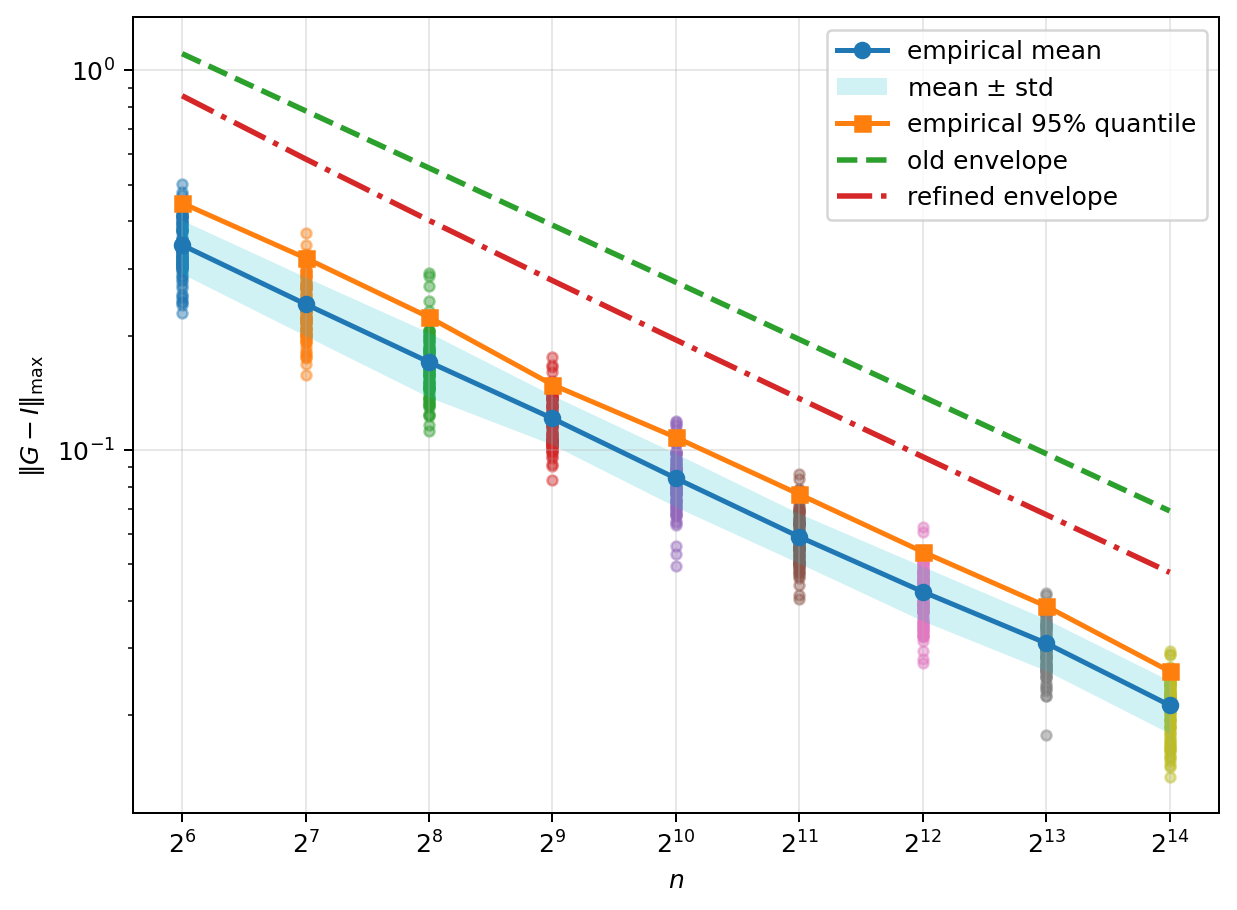
\includegraphics[width=\textwidth]{images/finite_sample_results/theory_envelope_compare_gram_err_max.png}
		\caption{\(\|G-I_d\|_{\max}\)}
	\end{subfigure}
	\hfill
	\begin{subfigure}[t]{0.48\textwidth}
		\centering
		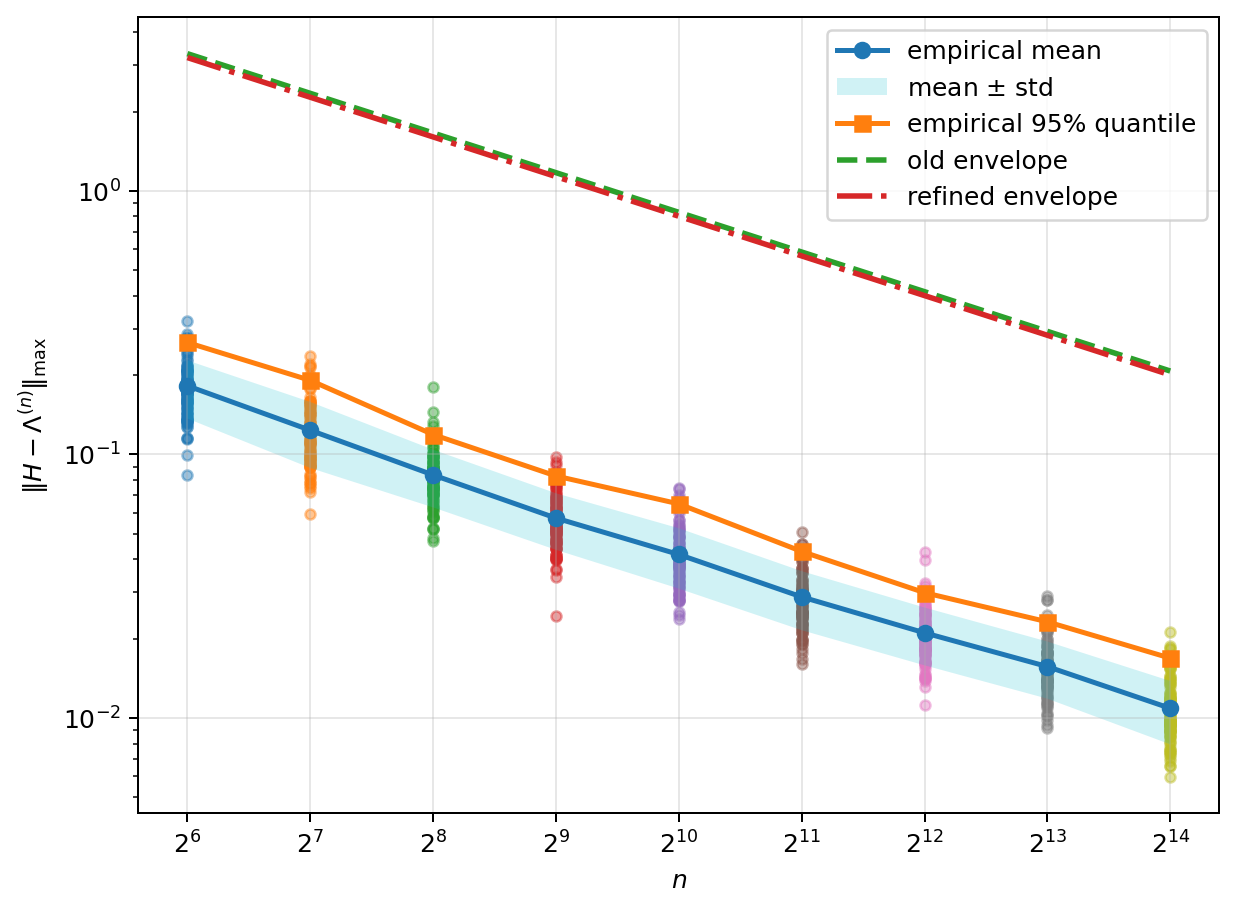
\includegraphics[width=\textwidth]{images/finite_sample_results/theory_envelope_compare_comp_err_max.png}
		\caption{\(\|H-\Lambda^{(n)}\|_{\max}\)}
	\end{subfigure}

	\vspace{0.8em}

	\begin{subfigure}[t]{0.48\textwidth}
		\centering
		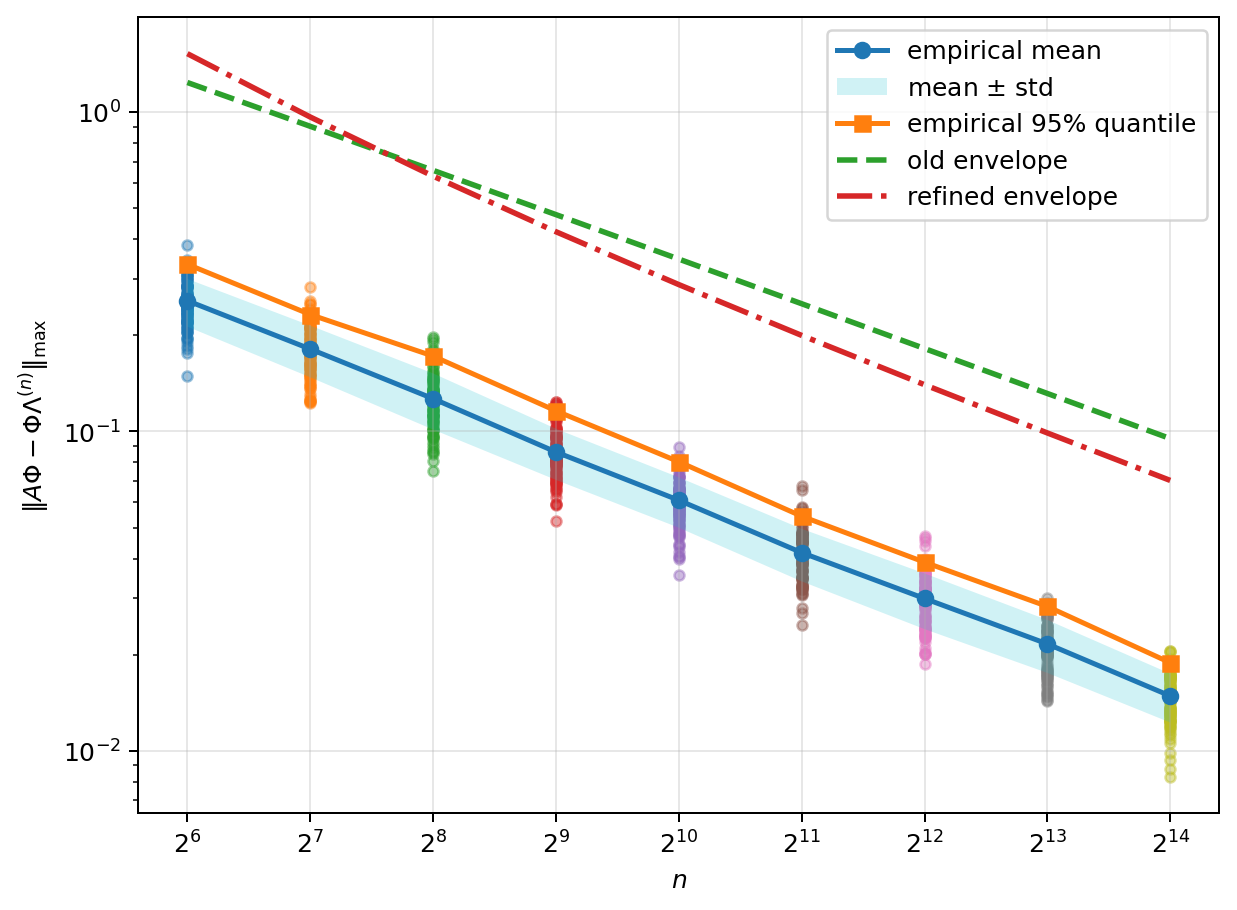
\includegraphics[width=\textwidth]{images/finite_sample_results/theory_envelope_compare_action_err_max.png}
		\caption{\(\|A\Phi-\Phi\Lambda^{(n)}\|_{\max}\)}
	\end{subfigure}

	\caption{Finite-sample diagnostics for the sampled Fourier approximation.
		The three plotted errors decrease with \(n\). The theoretical envelopes are
		conservative, but they show the same decreasing trend.}
	\label{fig:results-finite-sample-diagnostics}
\end{figure}

These bounds naturally lead to the question of what finite sampling does to the
residual dynamics. In the continuum setting,
\eqref{eq:results-continuum-gradient-flow-mode-decay} shows that Fourier
components decay independently. On the retained subspace, this gives the
coefficient system
\[
	\dot\alpha(t)=-\Lambda\alpha(t).
\]
After sampling, if the residual is mainly represented in the retained Fourier
span, then
\[
	\widehat r(t)\approx \Phi\alpha(t),
\]
and the sampled kernel dynamics
\[
	\dot{\widehat r}(t)=-A\widehat r(t)
\]
gives
\[
	\Phi\dot\alpha(t)\approx -A\Phi\alpha(t).
\]
Using the finite-sample decomposition
\[
	A\Phi
	=
	\Phi\Lambda^{(n)}
	+
	\bigl(A\Phi-\Phi\Lambda^{(n)}\bigr),
\]
we obtain
\[
	\Phi\dot\alpha(t)
	\approx
	\underbrace{-\Phi\Lambda^{(n)}\alpha(t)}
	_{\text{finite-sample eigenvalue prediction}}
	\underbrace{
		-\bigl(A\Phi-\Phi\Lambda^{(n)}\bigr)\alpha(t)
	}_{\text{finite-sample action error}} .
\]
If the action-error term were zero, each retained Fourier component would follow
\begin{equation}
	\alpha_p(t)
	=
	\exp(-\lambda_p^{(n)}t)\alpha_p(0)
	\label{eq:finite-sample-eigenvalue-prediction}
\end{equation}

The action-error term is small by the finite-sample bounds, but it is not zero.
To see when it can become visible, suppose that the retained coefficients are
normalized so that \(\alpha_p(0)=1\) for all retained basis indices \(p\) in \(\mathcal H_K\), and
suppose initially that they follow the finite-sample eigenvalue prediction from \eqref{eq:finite-sample-eigenvalue-prediction}.
Then
\[
	\alpha(t)
	\approx
	\exp(-\Lambda^{(n)}t)\mathbf 1,
\]
and hence
\[
	\widehat r(t)
	\approx
	\Phi\exp(-\Lambda^{(n)}t)\mathbf 1
	=
	\sum_p \exp(-\lambda_p^{(n)}t)\Phi_p,
\]
where \(\Phi_p\) is the sampled vector of the \(p\)-th retained Fourier basis
function and \(\mathbf 1\in\mathbb R^d\) is the vector with all entries equal to one.

Substituting this expression into the action-error term gives
\[
	\bigl(A\Phi-\Phi\Lambda^{(n)}\bigr)\alpha(t)
	\approx
	\bigl(A\Phi-\Phi\Lambda^{(n)}\bigr)
	\exp(-\Lambda^{(n)}t)\mathbf 1 .
\]
Therefore
\[
	\left\|
	\bigl(A\Phi-\Phi\Lambda^{(n)}\bigr)\alpha(t)
	\right\|_{\max}
	\le
	\|A\Phi-\Phi\Lambda^{(n)}\|_{\max}
	\sum_p \exp(-\lambda_p^{(n)}t).
\]
This is a crude upper bound on the extra motion caused by finite sampling, and gives a scale at which
deviations from the predicted eigenvalue decay become visible.

For a single retained component \(p\), the eigenvalue prediction gives
\[
	|\alpha_p(t)|
	\approx
	\exp(-\lambda_p^{(n)}t),
	\qquad
	|\dot\alpha_p(t)|
	\approx
	\lambda_p^{(n)}\exp(-\lambda_p^{(n)}t).
\]
Thus, the predicted movement of component \(p\) is \(\lambda_p^{(n)}\exp(-\lambda_p^{(n)}t)\).
This eigenvalue prediction should therefore be reliable while
\[
	\lambda_p^{(n)}\underbrace{\exp(-\lambda_p^{(n)}t)}_{\alpha_p(t)}
	\gg
	\|A\Phi-\Phi\Lambda^{(n)}\|_{\max} \sum_q \underbrace{\exp(-\lambda_q^{(n)}t)}_{\alpha_q(t)}.
\]

The left-hand side is the motion predicted for component \(p\) by its own eigenvalue.
This term becomes small as \(\alpha_p(t)\) decays.
The right-hand side is a bound on the extra motion coming from the
finite-sample action error. This term is small when the action error is small,
but it depends on all retained components, including components that decay more
slowly.

The comparison above suggests a two-stage picture. At early times, the
retained components have not yet decayed much, so the eigenvalue-driven motion
is larger than the finite-sample action error. The sampled curves should
therefore follow the finite-sample eigenvalue prediction. At later times, after
some components have decayed substantially, the same action error can become
visible relative to the remaining motion. Figures~\ref{fig:results-random-sampling-first200}
and~\ref{fig:results-random-sampling-highfreq} show these two regimes for
\(n=4096\) uniformly sampled points.

\begin{figure}[!htbp]
	\centering
	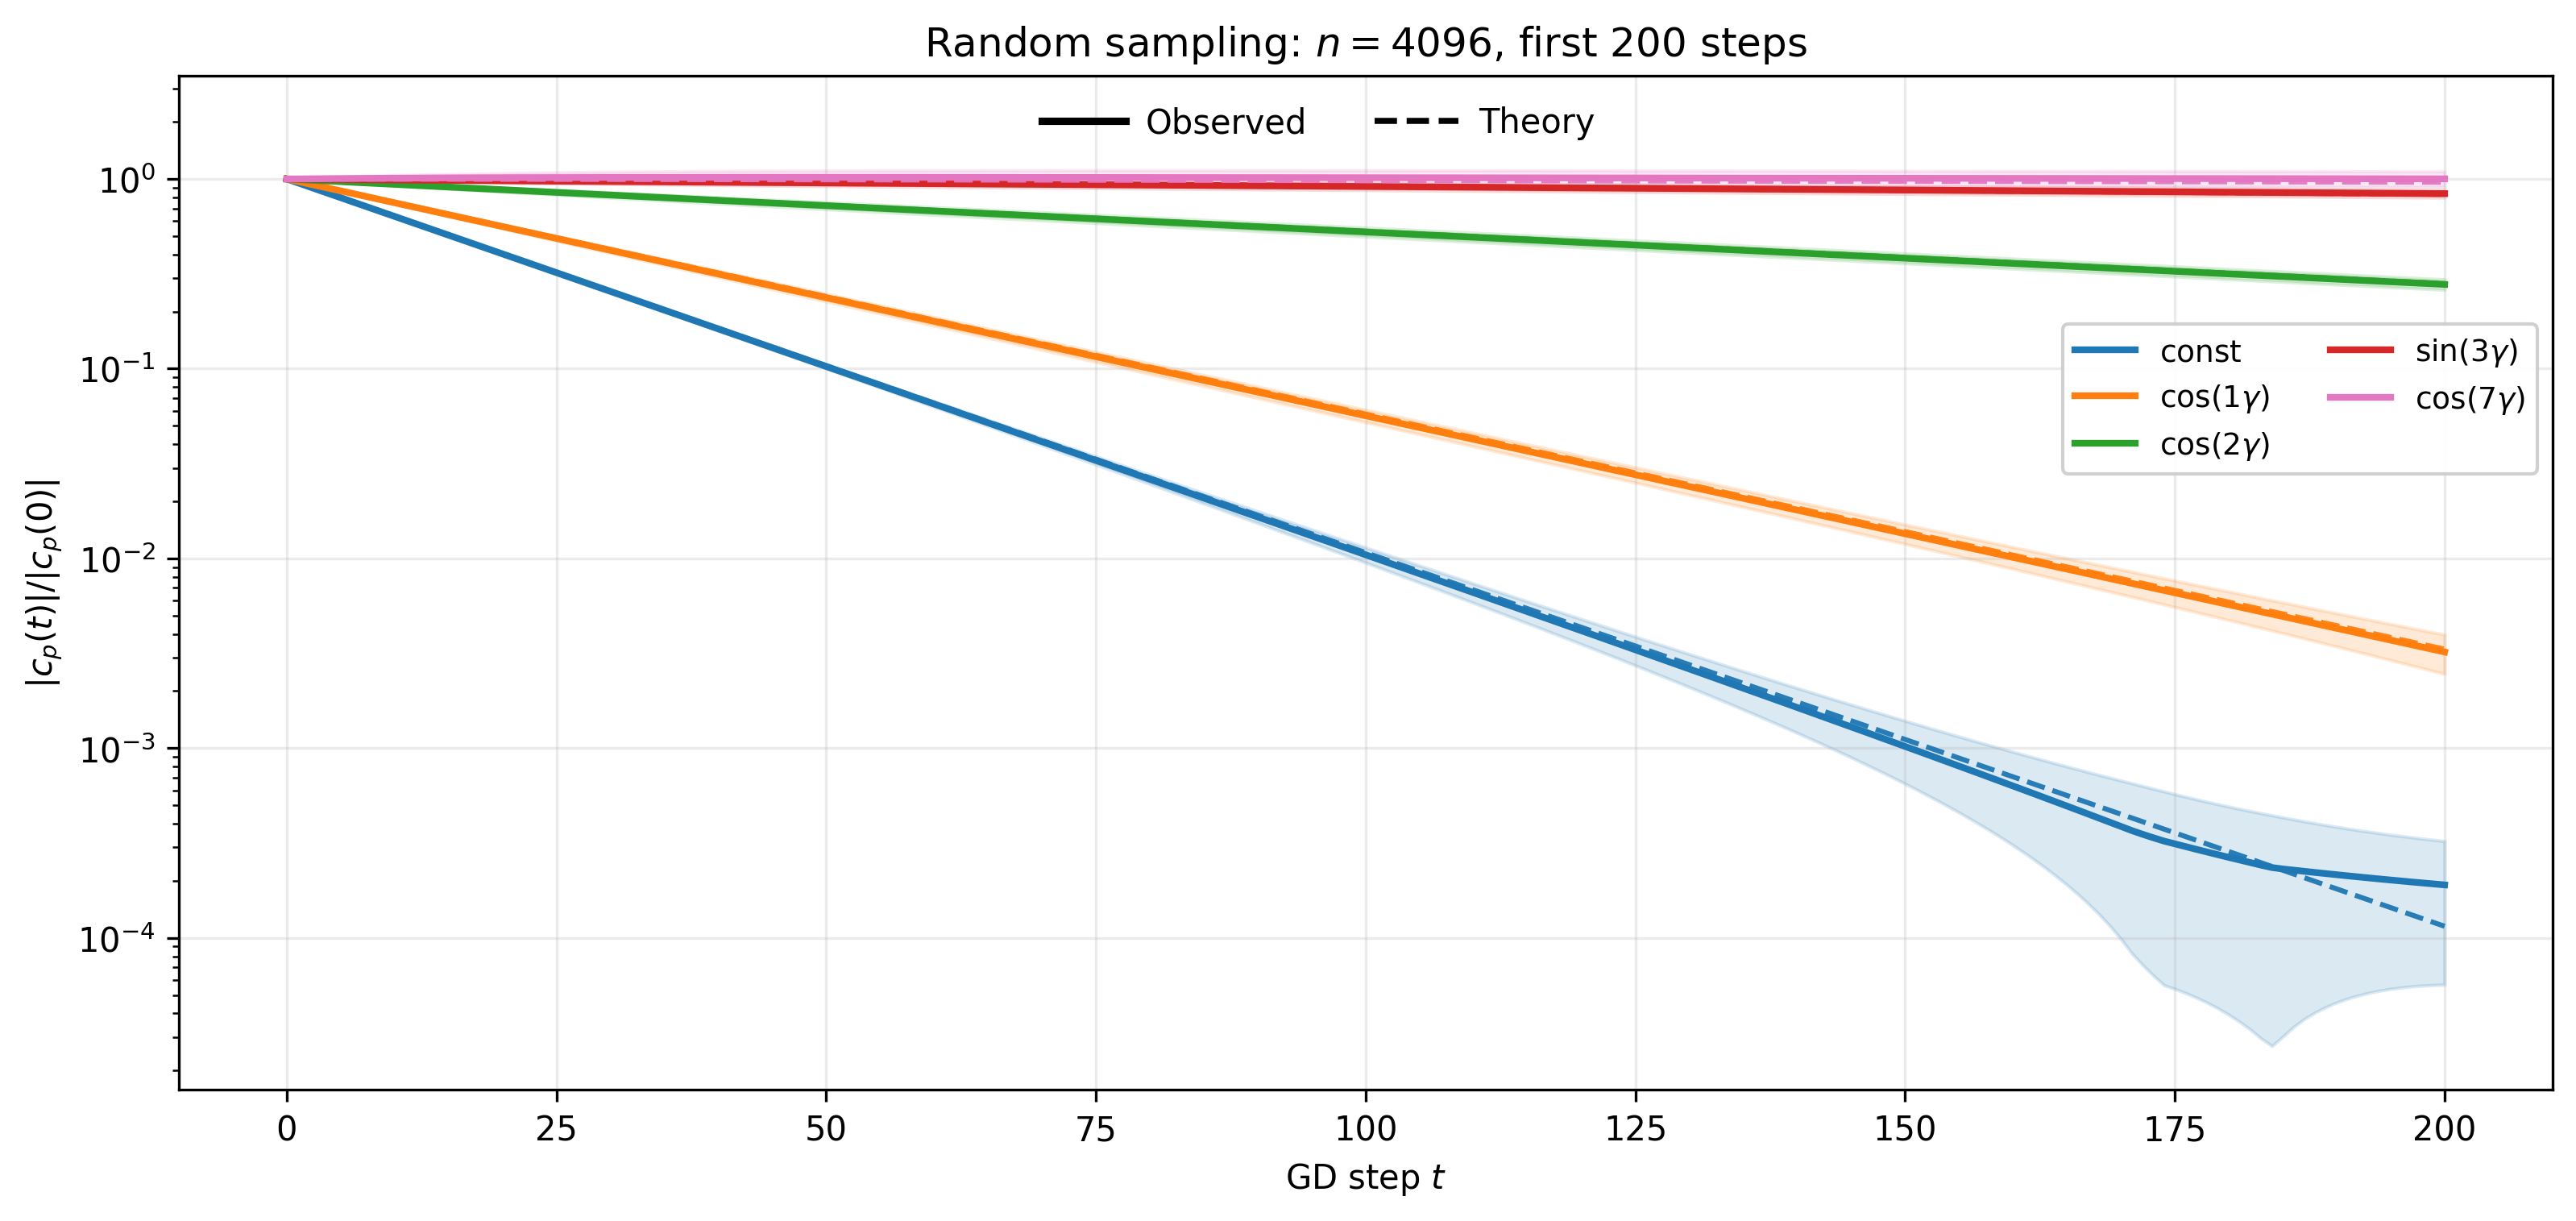
\includegraphics[width=\textwidth]{images/finite_sample_results/story_02_random_n4096_components_first200.png}
	\caption{Random sampling with \(n=4096\), first \(200\) gradient descent
		steps. Solid curves show the observed normalized residual amplitudes
		\(|\alpha_p(t)|/|\alpha_p(0)|\), while dashed curves show the diagonal
		prediction from the finite-sample corrected eigenvalues
		\(\lambda_p^{(n)}\).}
	\label{fig:results-random-sampling-first200}
\end{figure}

\begin{figure}[!htbp]
	\centering
	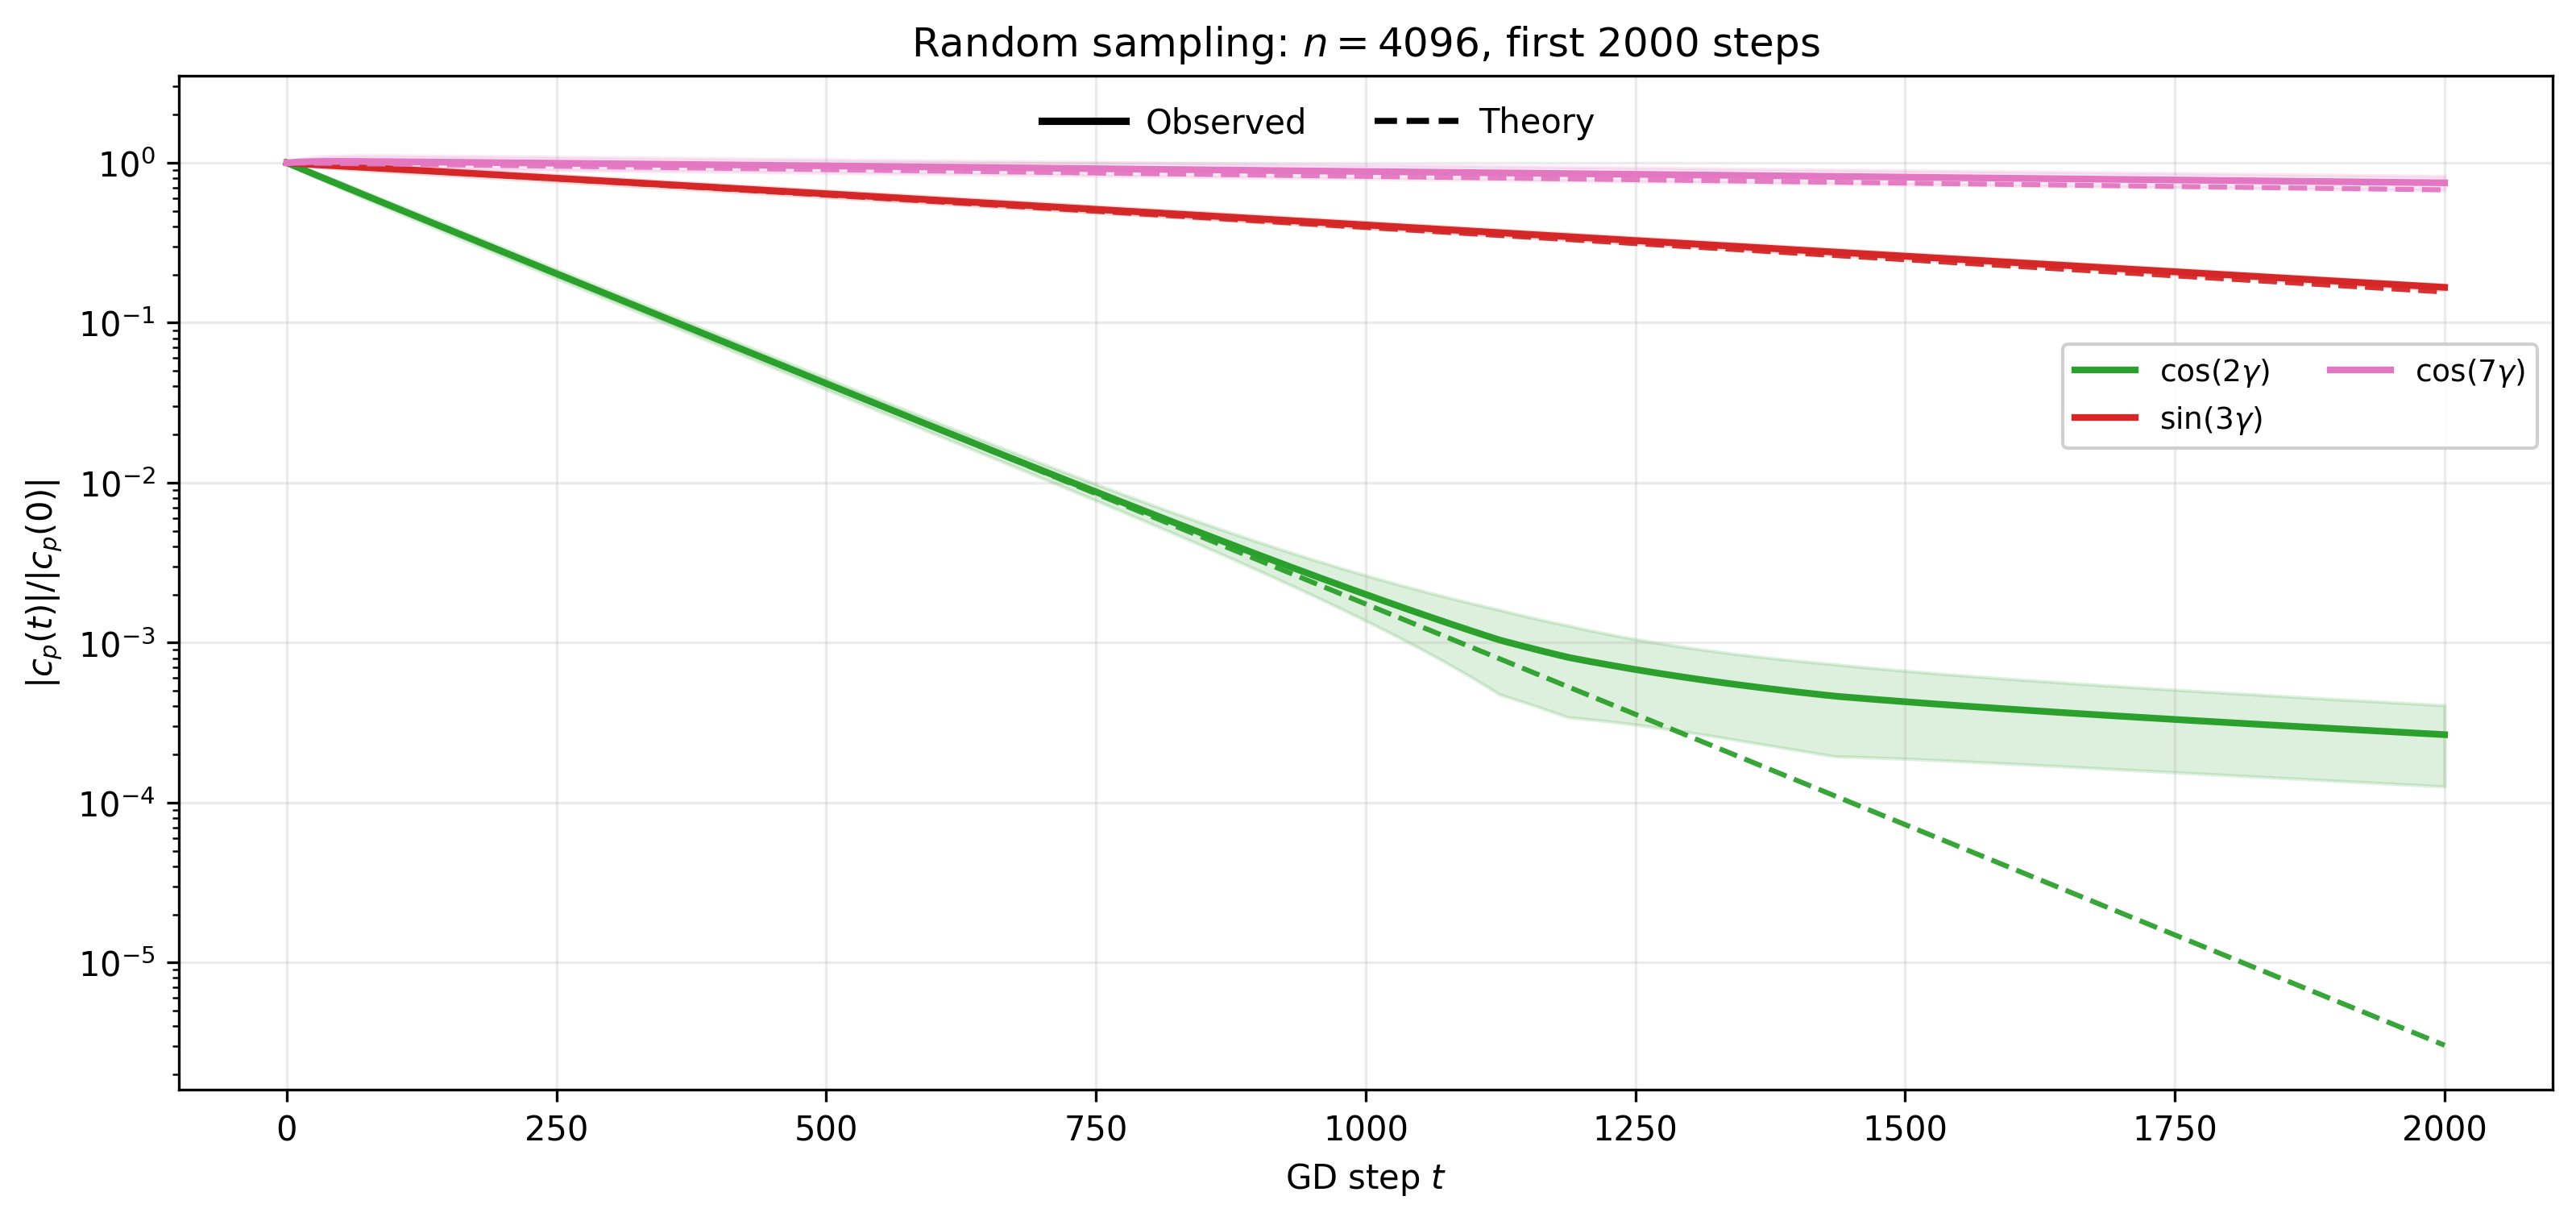
\includegraphics[width=\textwidth]{images/finite_sample_results/story_02_random_n4096_components_all_steps_high_freq_only.png}
	\caption{Random sampling with \(n=4096\), higher-frequency retained modes over
		\(2000\) gradient descent steps. The diagonal prediction captures the initial
		decay rates, while small deviations from this prediction become visible at
		later times.}
	\label{fig:results-random-sampling-highfreq}
\end{figure}

However, the level at which an individual curve starts to flatten cannot be computed
directly from the max-norm bounds in
Theorem~\ref{thm:results-finite-sample-concentration} because these bounds control the
largest possible error over the whole retained Fourier block. They are
therefore useful for explaining why deviations can appear once the predicted
motion becomes small, but they do not determine the deviation level of each
Fourier component separately. That level depends on the actual sampled operator
for the particular draw of training points, and on which other Fourier
components are still present when the component under consideration has already
decayed.

\subsection{Interpretation of the finite-sample results}
\label{subsec:results-finite-sample-interpretation}

The finite-sample results show that the continuum Fourier picture is not only a
population-level statement. For a fixed low-frequency block \(\mathcal H_K\),
random sampling perturbs the Fourier structure in a controlled way. The sampled
basis is not exactly orthonormal, and the sampled Fourier modes are not exact
eigenvectors of the sampled operator, but the errors measured by
\(G-I_d\), \(H-\Lambda^{(n)}\), and
\(A\Phi-\Phi\Lambda^{(n)}\) decrease with \(n\).

This supports the usual NTK spectral-bias mechanism in a finite-sample setting.
In the continuum model, the Fourier modes diagonalize the NTK operator and the
eigenvalues determine the decay rates. The results above show that, on a fixed
retained block, the sampled operator remains close to this diagonal Fourier
description. This complements the population-level harmonic analyses of NTK
spectra on the sphere and circle
\citep{basri2019convergence,bietti2019inductivebiasneuraltangent,
	cao2020understandingspectralbiasdeep,basri2020frequencybiasneuralnetworks}
by making explicit how the same structure survives after replacing the uniform
measure by finitely many sampled points.

The residual experiments then show the dynamical consequence. The corrected
finite-sample eigenvalues \(\lambda_p^{(n)}\) predict the early decay of the
retained Fourier components, while the finite-sample action error explains why
late-time deviations can appear once some components have become small. Thus
finite sampling does not remove the spectral-bias mechanism; it turns the exact
continuum diagonal dynamics into an approximate low-frequency description.

This suggests a direct test. If the decay of each retained component is mainly
governed by its eigenvalue, then an eigenvalue-based rescaling should
remove most of the frequency-dependent decay. The next experiment tests this prediction directly.

\section{Preconditioned sampled dynamics}
\label{sec:results-preconditioned-sampled-dynamics}

We next apply the Fourier-block preconditioning construction from
Section~\ref{sec:method-preconditioning}. The goal is to compare the baseline
sampled dynamics with two block-corrected dynamics: one using the diagonal
finite-sample prediction and one using the observed sampled Fourier block.

\subsection{Experimental setup}
\label{subsec:results-preconditioned-setup}

The three sampled dynamics are
\[
	B_{\mathrm{base}}=A,
	\qquad
	B_{\mathrm{th}}=P_{\mathrm{th}}A,
	\qquad
	B_{\mathrm{emp}}=P_{\mathrm{emp}}A.
\]
Here \(P_{\mathrm{th}}\) is defined in
\eqref{eq:method-theory-preconditioner} and uses the diagonal prediction
\(\Lambda^{(n)}\). The empirical preconditioner \(P_{\mathrm{emp}}\), defined in
\eqref{eq:method-empirical-preconditioner}, uses the observed coefficient-space
block \(C_n^{(K)}=G^{-1}H\).

In this experiment, we use the target
\begin{equation}
	f^*(\gamma)
	=
	1
	+0.9\cos(\gamma)
	+0.5\cos(2\gamma)
	-0.35\sin(3\gamma)
	+0.25\cos(7\gamma).
	\label{eq:results-preconditioned-in-block-target}
\end{equation}
The retained preconditioning block contains all active target frequencies shown
in the residual plots.

\subsection{Mode-wise residual decay}
\label{subsec:results-preconditioned-mode-decay}

Figure~\ref{fig:results-preconditioned-mode-decay} shows the
residual amplitudes for the baseline, theory-preconditioned, and empirically
preconditioned dynamics. The baseline dynamics show separated decay rates
across retained modes. Both preconditioned dynamics reduce this separation, with
the empirical preconditioner giving the flattest curves.

\begin{figure}[!htbp]
	\centering
	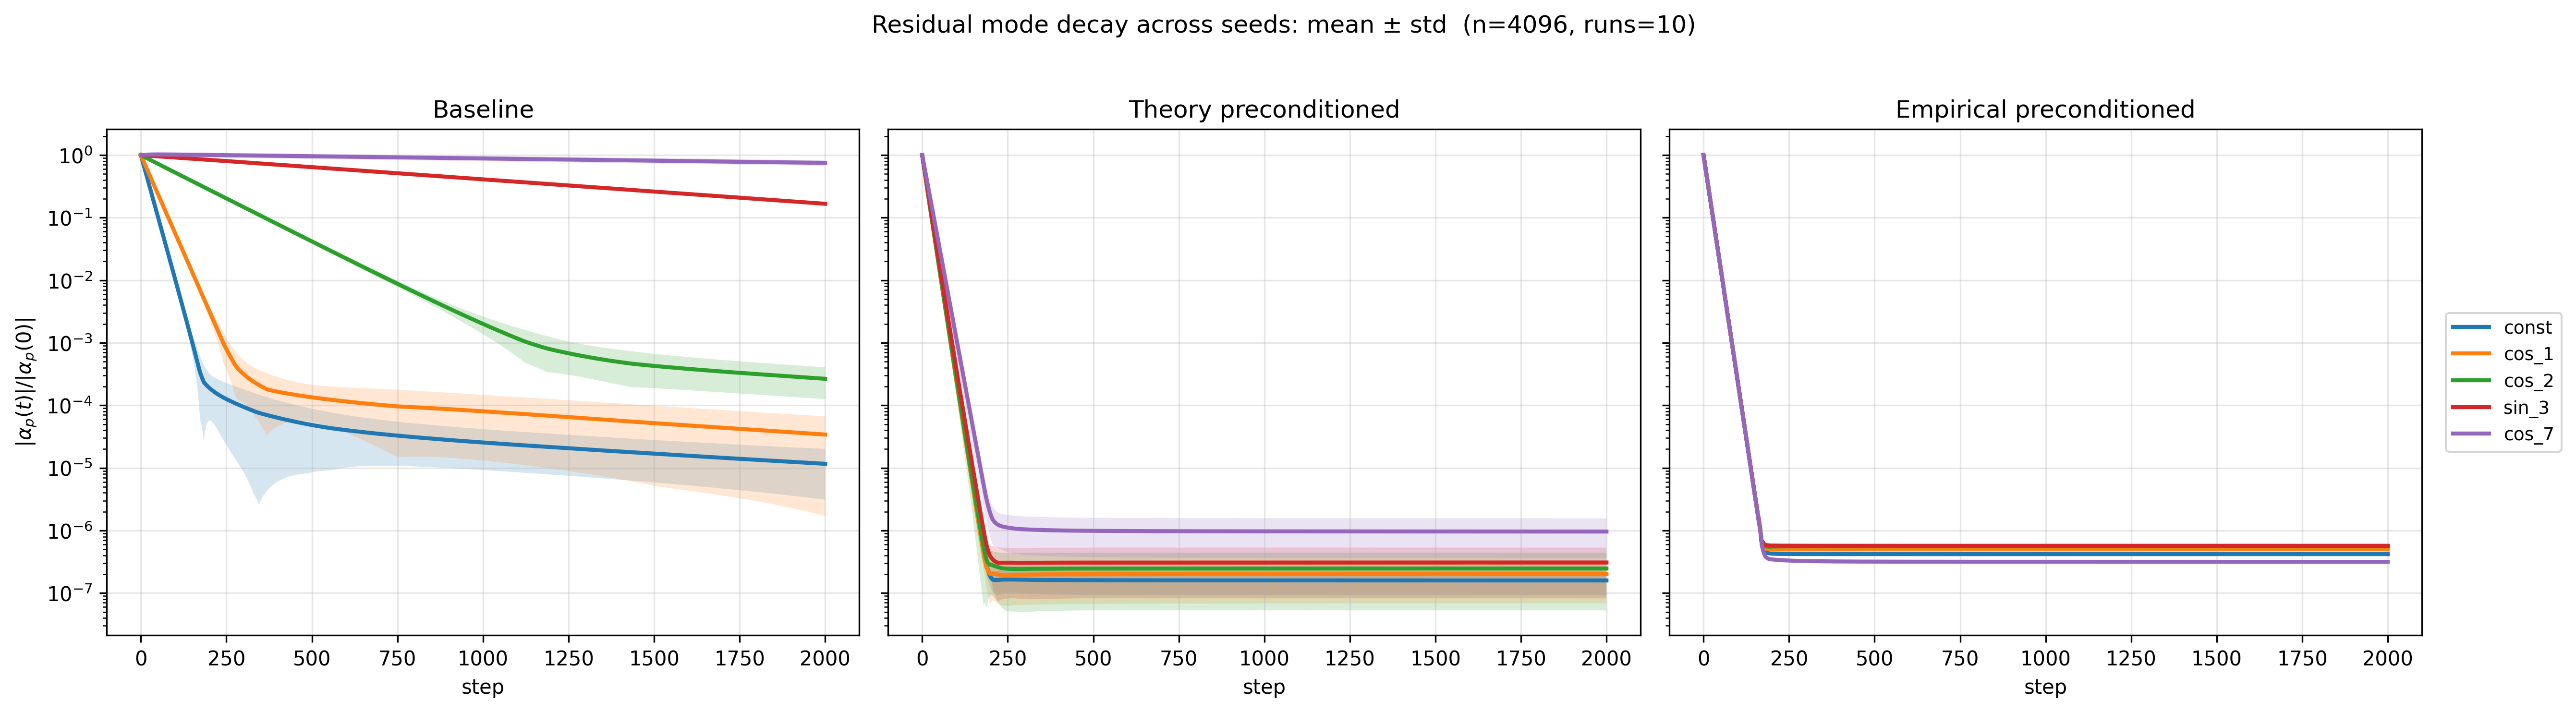
\includegraphics[width=\textwidth]{images/finite_sample_results/all_mode_decay_three_panel_mean_std_n4096.png}
	\caption{Preconditioned sampled dynamics at \(n=4096\). The baseline dynamics
		shows separated decay rates across retained Fourier modes. Both
		preconditioned dynamics make the retained residual amplitudes decay on more
		similar time scales. The empirical preconditioner gives the most uniform
		decay, while the theory preconditioner uses only the predicted diagonal
		scaling.}
	\label{fig:results-preconditioned-mode-decay}
\end{figure}

Figure~\ref{fig:results-preconditioned-probe-fit} compares the final prediction
on a dense probe grid. The baseline fit leaves a visible residual, while both
preconditioned flows more closely match the target.

\begin{figure}[!htbp]
	\centering
	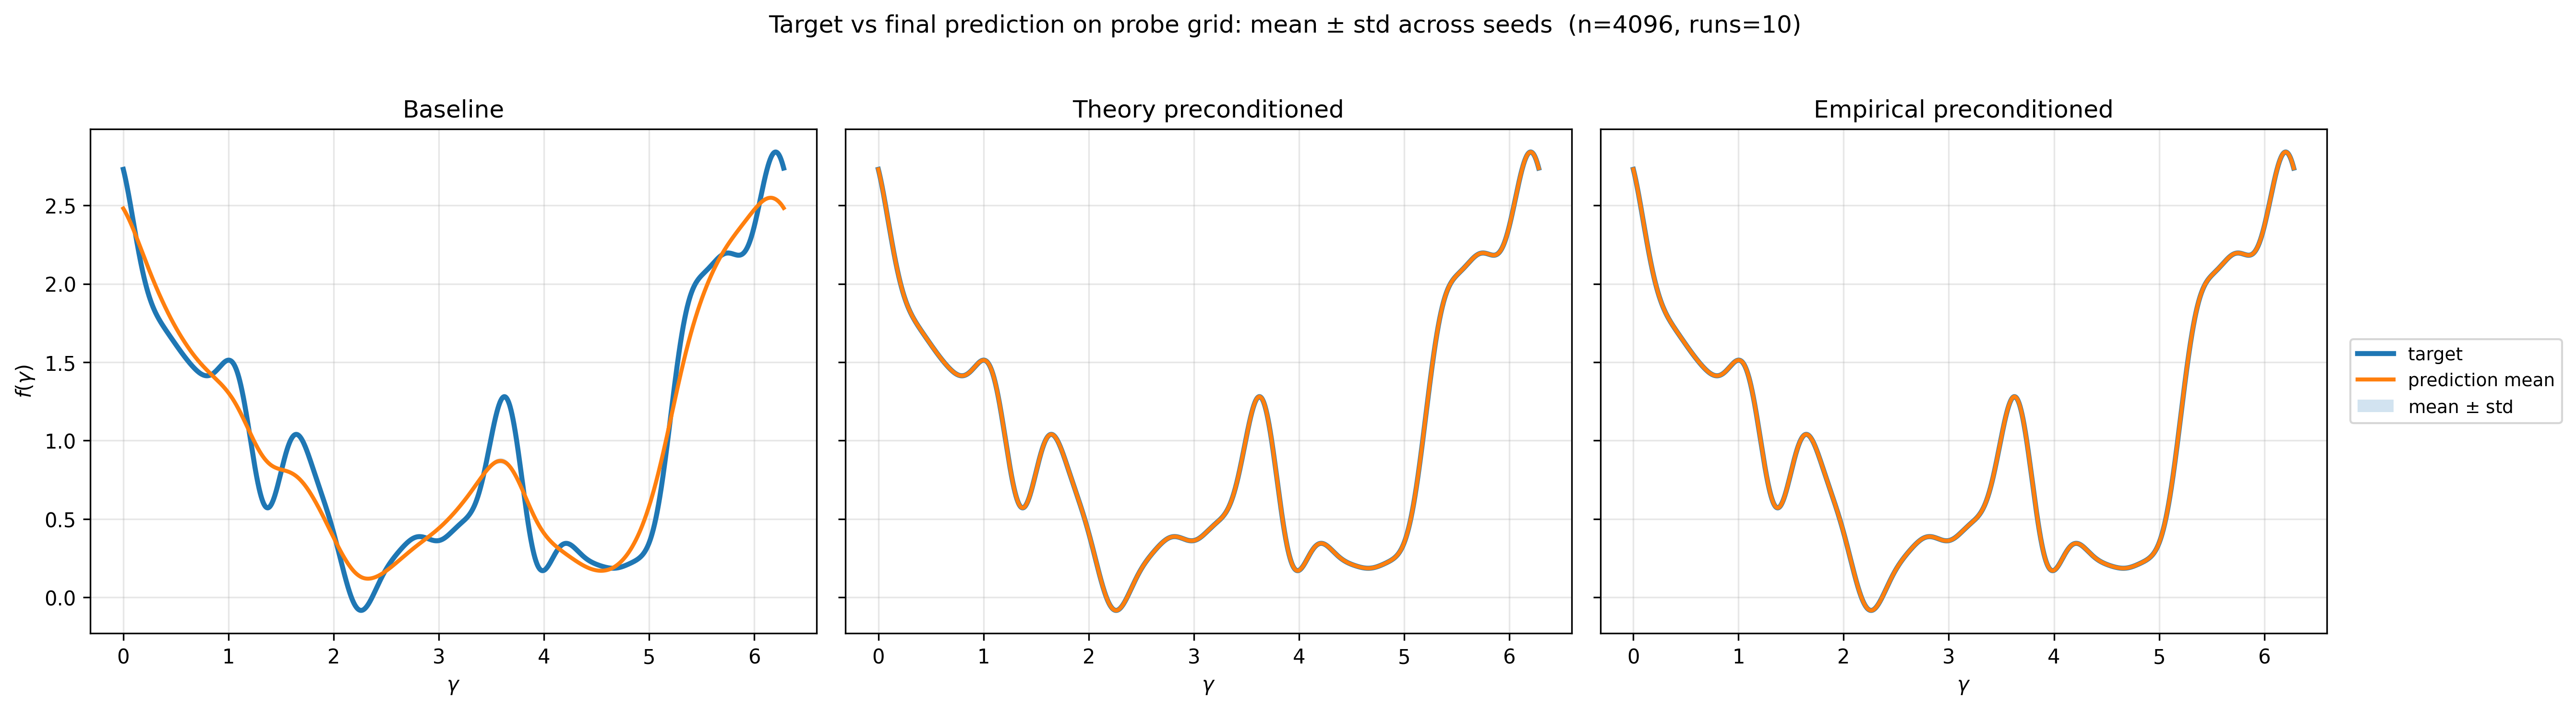
\includegraphics[width=\textwidth]{images/finite_sample_results/probe_target_vs_prediction_three_panel_mean_std_n4096.png}
	\caption{Final prediction on a dense probe grid for the same experiment as
		Figure~\ref{fig:results-preconditioned-mode-decay}. The baseline fit leaves a
		visible residual, while both preconditioned dynamics closely match the target.
		The theory and empirical preconditioners are nearly indistinguishable at the
		level of the final fitted function.}
	\label{fig:results-preconditioned-probe-fit}
\end{figure}

\subsection{Theory versus empirical preconditioning}
\label{subsec:results-theory-vs-empirical-preconditioning}

Figure~\ref{fig:results-theory-precond-spectrum} shows the spectrum obtained
after applying the theory preconditioner to the sampled Fourier block. At the
coefficient level, the empirical block is \(C=G^{-1}H\). The empirical
preconditioner would invert this block directly, giving \(C_{\mathrm{emp}}^{-1}C=I_d\),
so all eigenvalues would be equal to \(1\). The theory preconditioner instead rescales
by the predicted diagonal eigenvalues \(\Lambda^{(n)}\). Thus it is exact only
when \(C=\Lambda^{(n)}\). The figure shows that, as \(n\) increases, the
theory-preconditioned spectrum moves closer to the ideal value \(1\). This is
the empirical counterpart of the finite-sample bounds above: the sampled block
\(C\) approaches the diagonal prediction \(\Lambda^{(n)}\), so the diagonal
theory preconditioner becomes a better approximation to the empirical block
inverse.

\begin{figure}[!htbp]
	\centering
	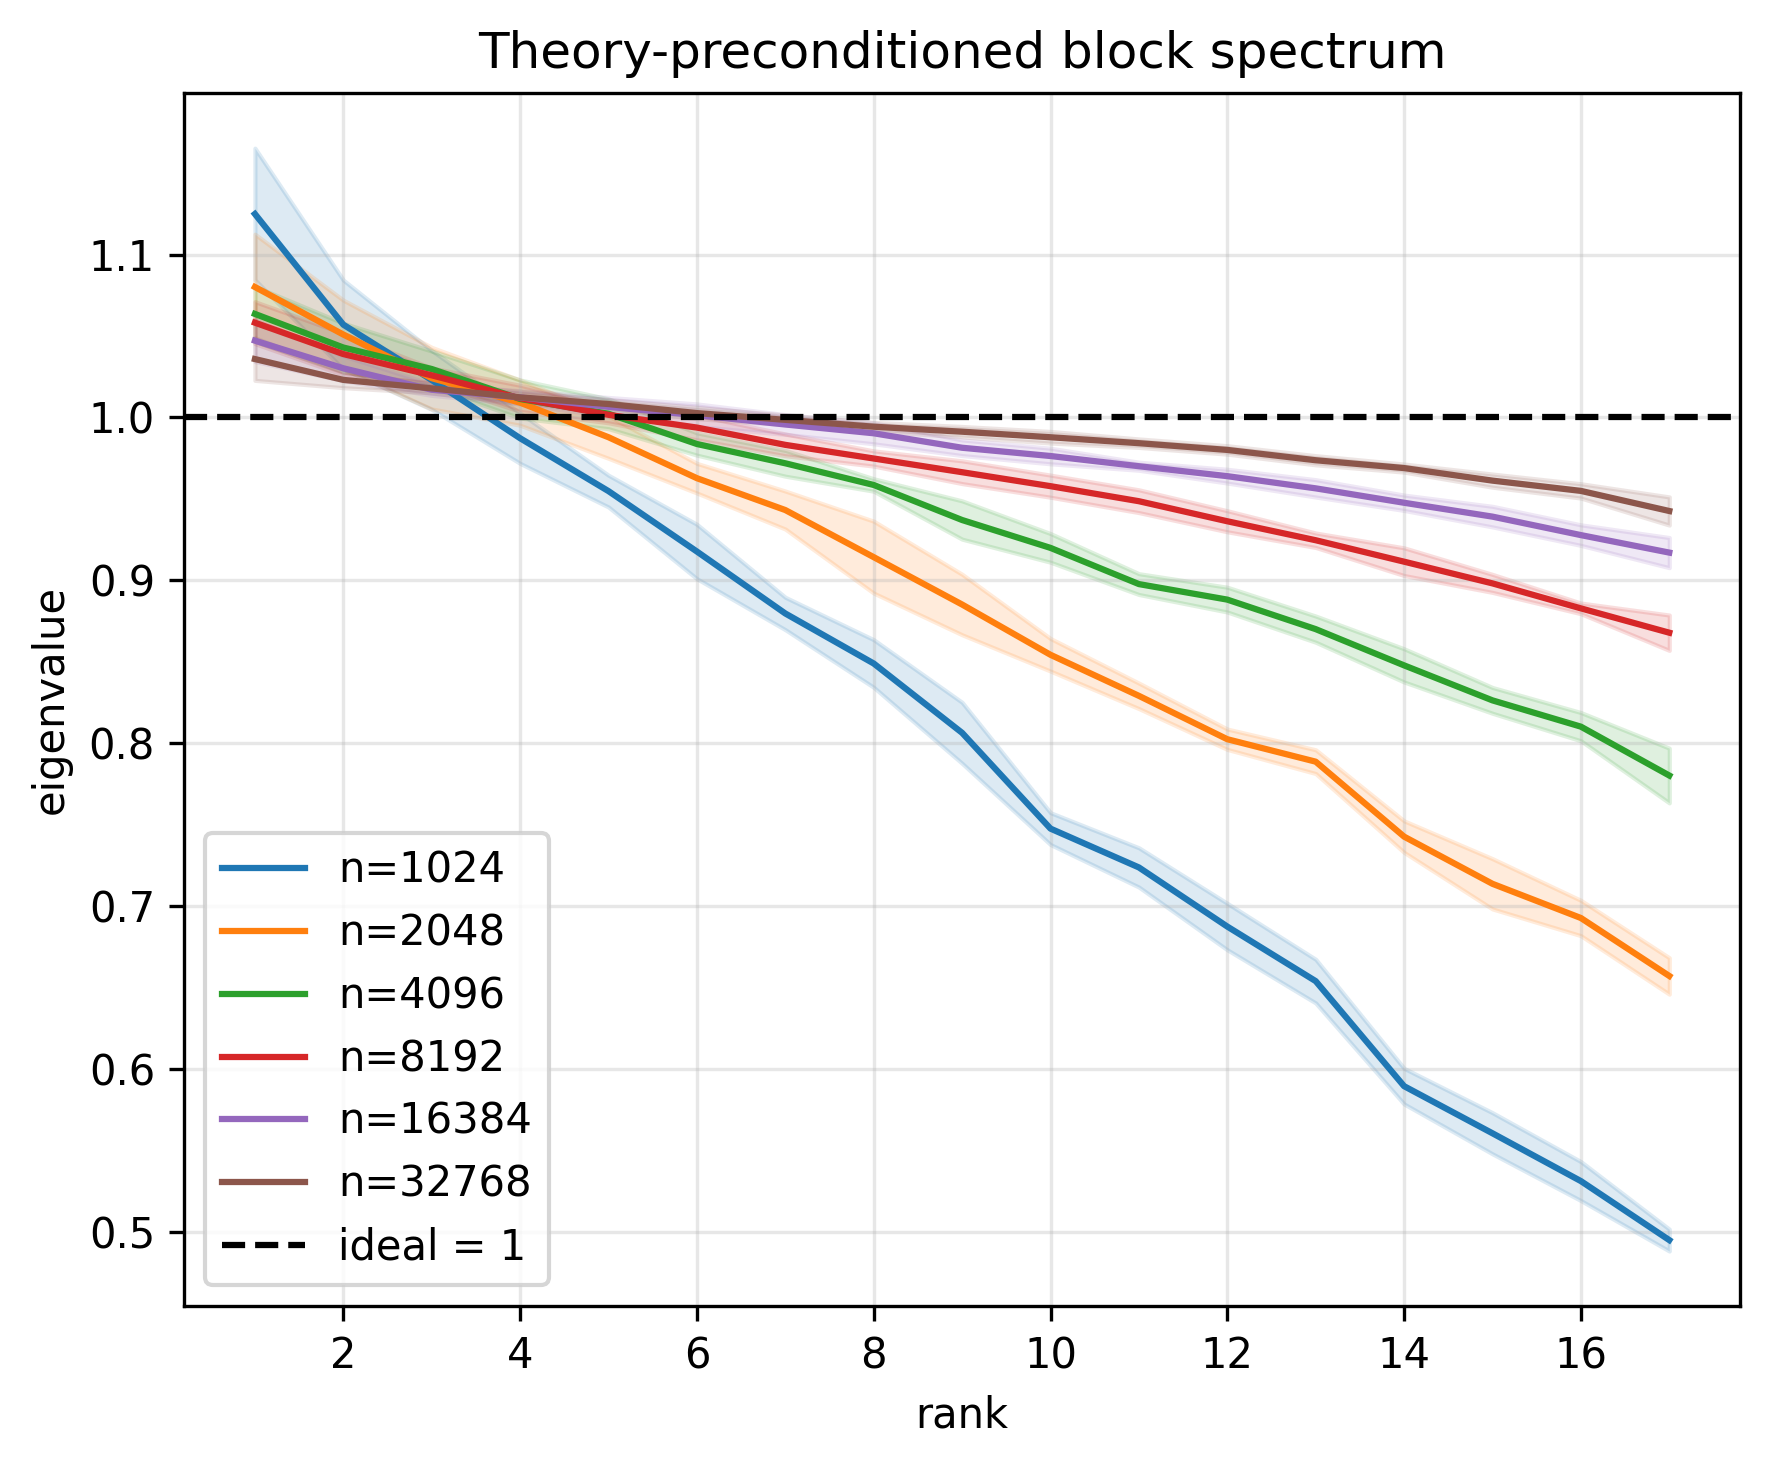
\includegraphics[width=0.72\textwidth]{images/finite_sample_results/theory_preconditioned_spectrum_all_n.png}
	\caption{Spectrum of the theory-preconditioned sampled Fourier block as a
		function of sample size. If the theory preconditioner exactly inverted the
		sampled block, all eigenvalues would be equal to \(1\). As \(n\) increases,
		the spectrum becomes flatter and moves closer to this ideal value.}
	\label{fig:results-theory-precond-spectrum}
\end{figure}

Figure~\ref{fig:results-preconditioner-gap} compares the theory and empirical
constructions at two levels. The preconditioner \(P\) is an operator on sampled
function values. Given a vector in \(\mathbb R^n\), it projects that vector onto
the retained Fourier block, rescales the retained Fourier coefficients, and
maps the result back to \(\mathbb R^n\). Thus, the gap between
\(P_{\mathrm{th}}\) and \(P_{\mathrm{emp}}\) measures how different the two
correction steps are before they are combined with the sampled kernel operator.

The product \(PA\) is the operator that is actually used in the residual
dynamics. It first applies the sampled kernel operator \(A\) to the residual,
and then applies the correction \(P\) to the retained Fourier components of the
result. Thus, the gap between \(B_{\mathrm{th}}\) and \(B_{\mathrm{emp}}\)
measures how different the resulting training dynamics are. Both gaps decrease
with sample size.

\begin{figure}[!htbp]
	\centering

	\begin{subfigure}[t]{0.48\textwidth}
		\centering
		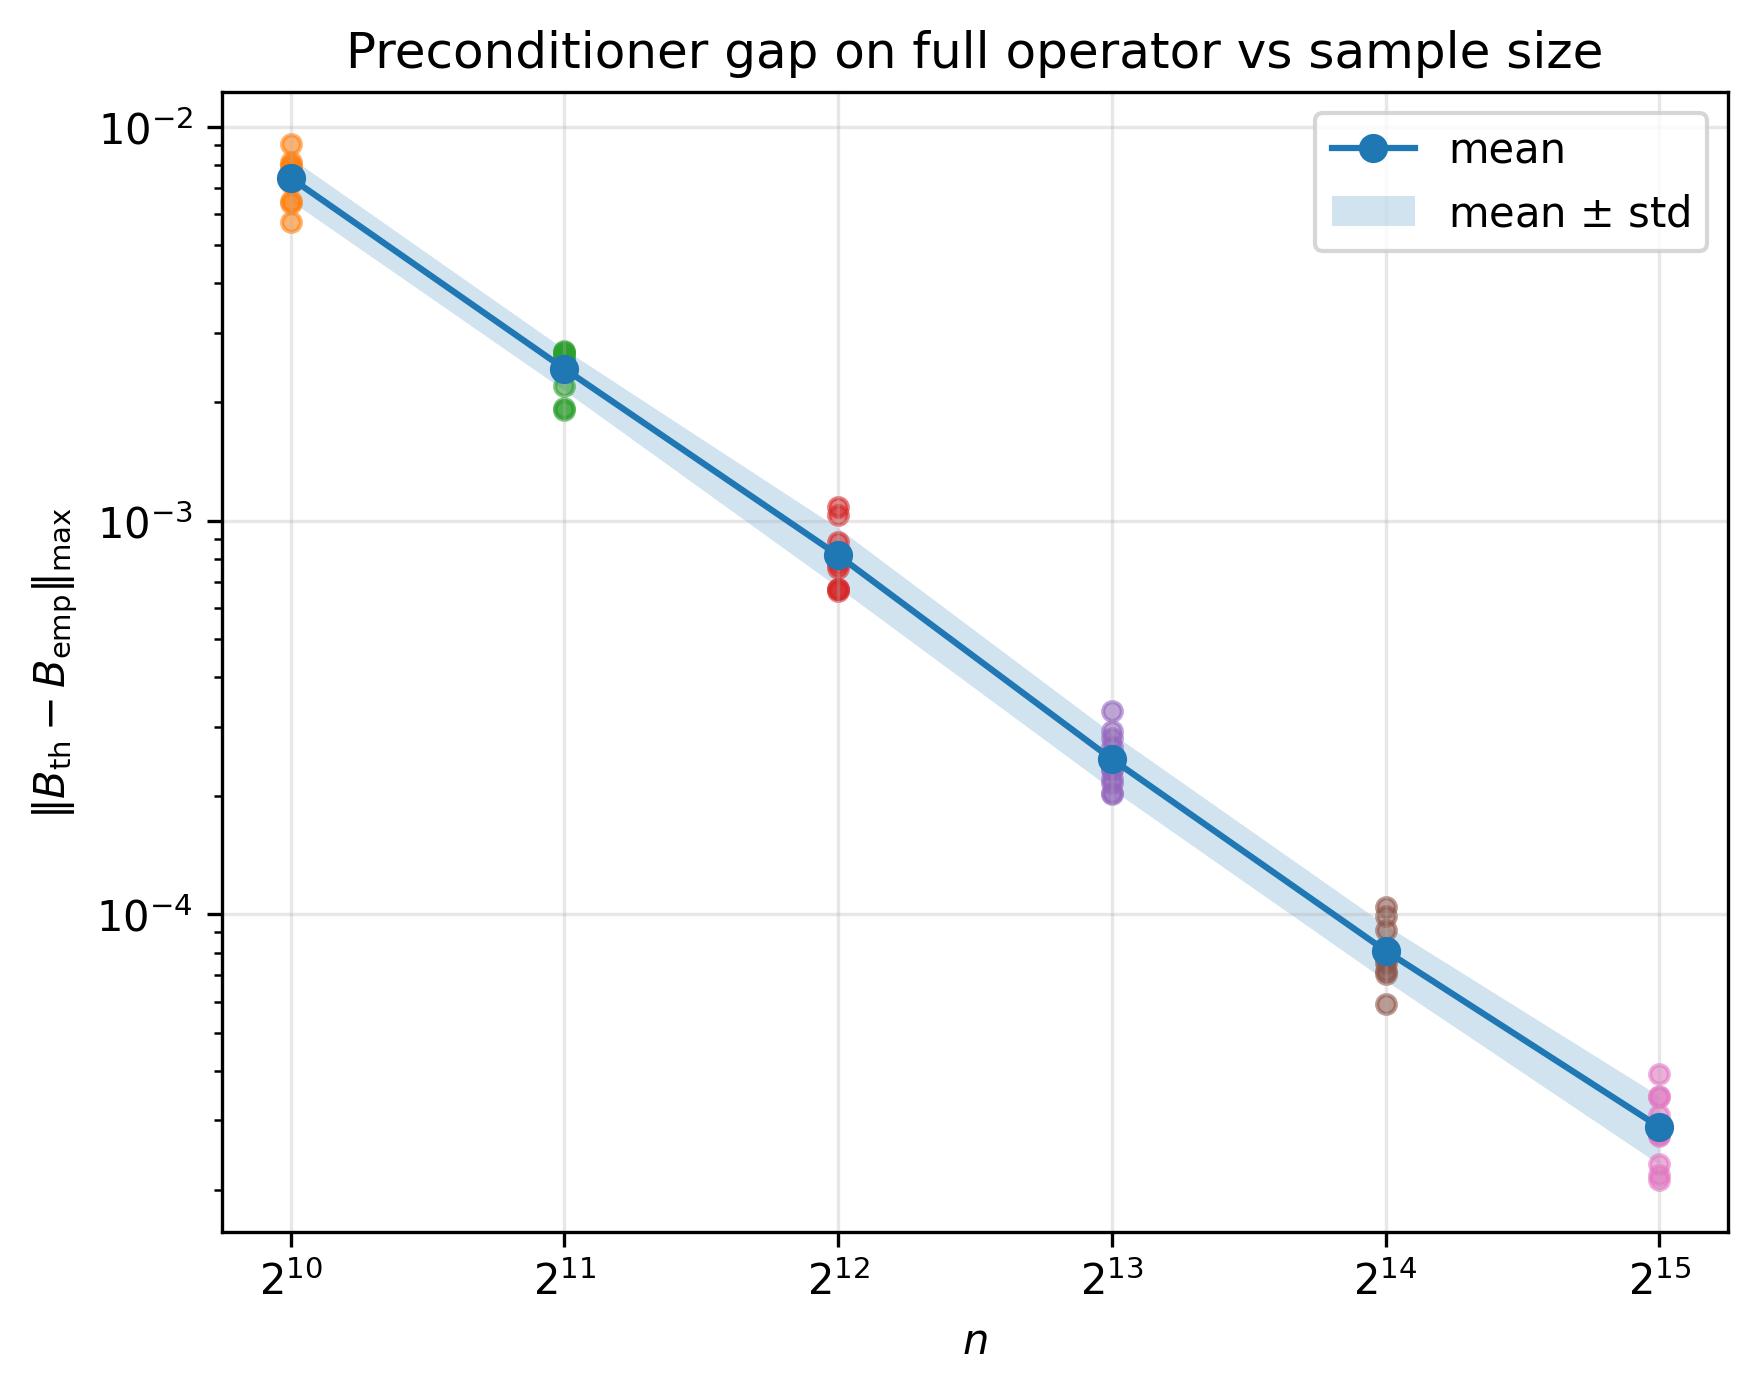
\includegraphics[width=\textwidth]{images/finite_sample_results/precond_diagnostic_B_th_vs_emp_max.png}
		\caption{\(\|B_{\mathrm{th}}-B_{\mathrm{emp}}\|_{\max}\)}
	\end{subfigure}
	\hfill
	\begin{subfigure}[t]{0.48\textwidth}
		\centering
		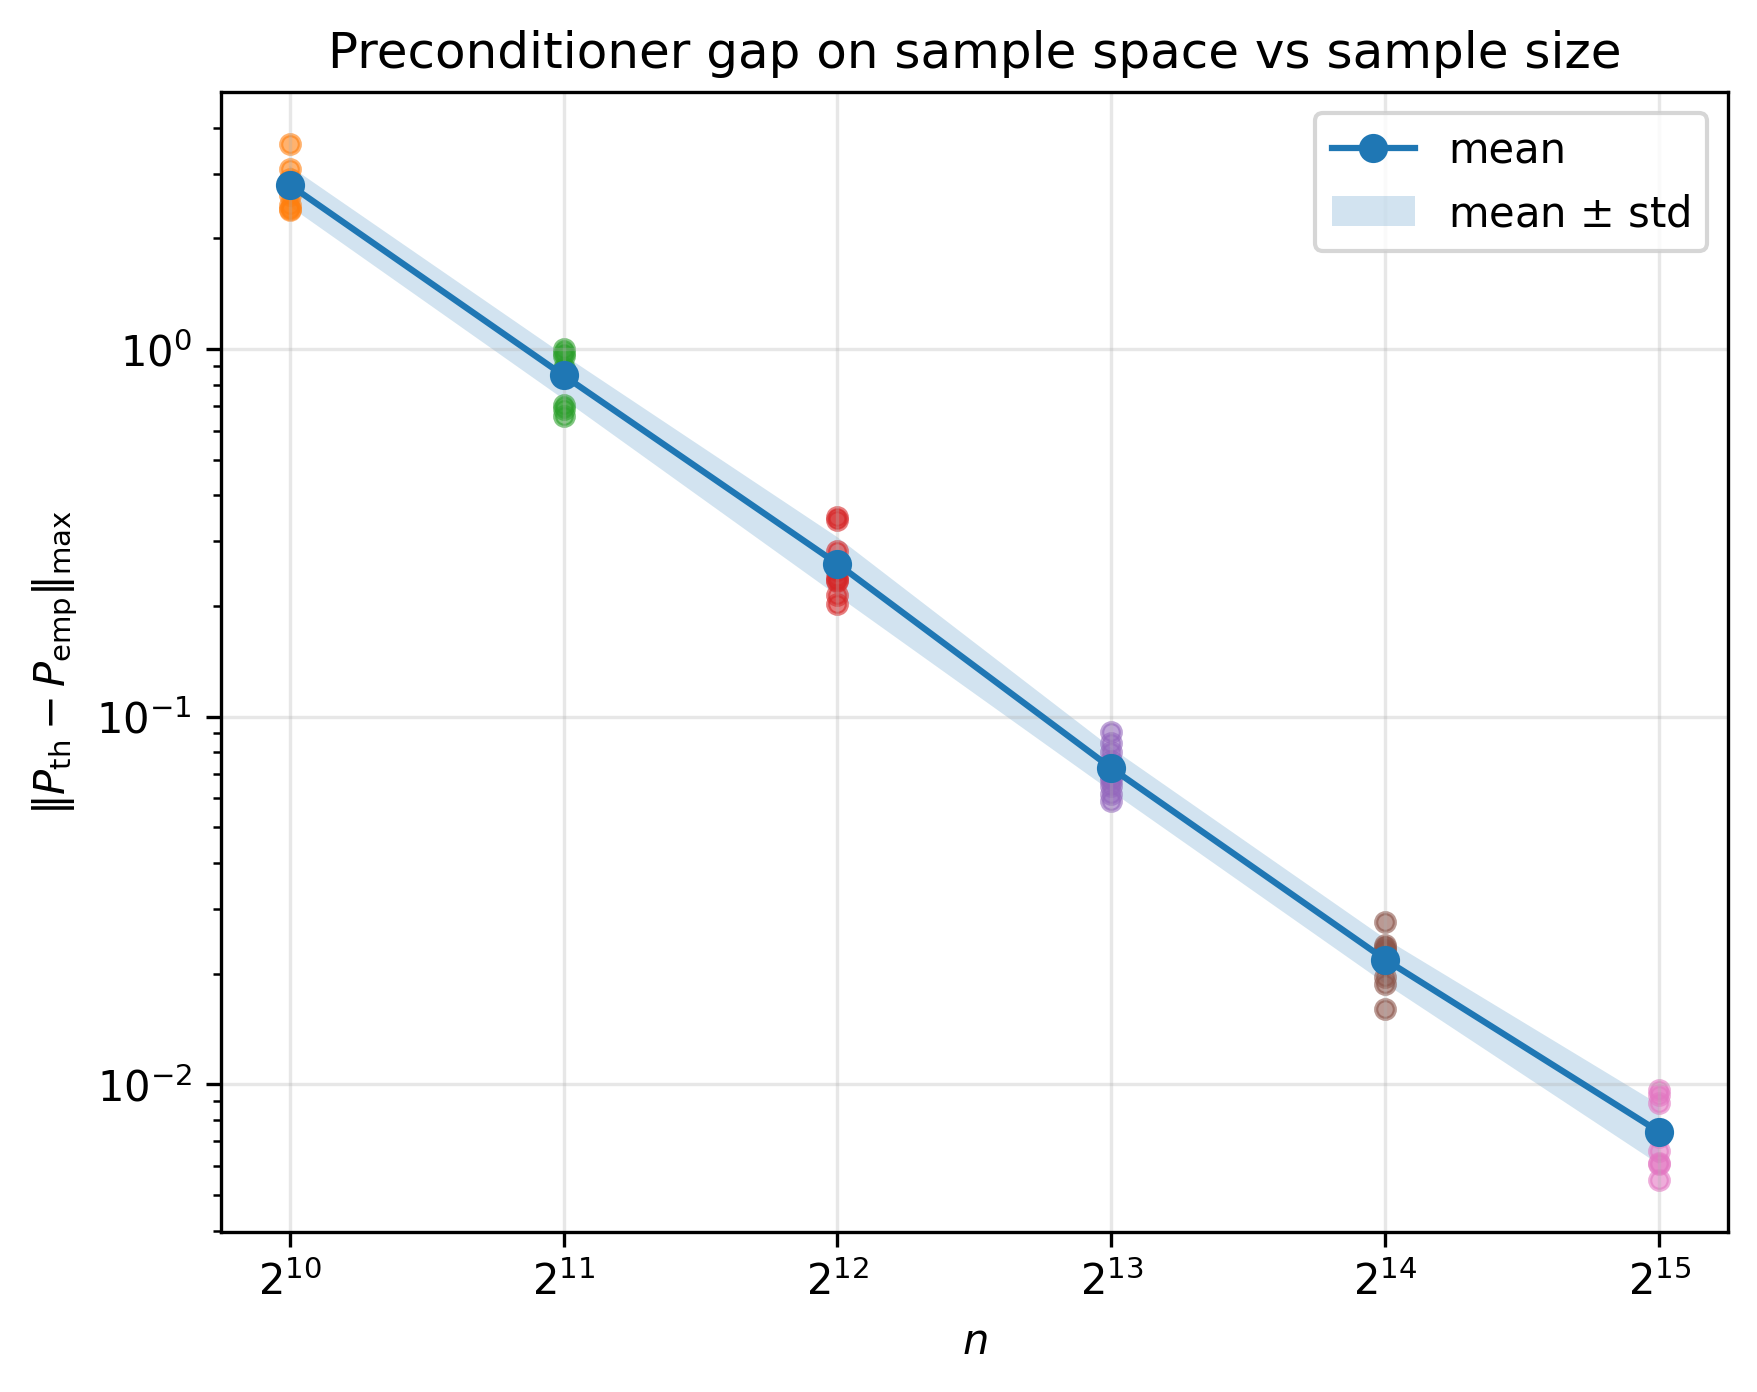
\includegraphics[width=\textwidth]{images/finite_sample_results/precond_diagnostic_P_th_vs_emp_max.png}
		\caption{\(\|P_{\mathrm{th}}-P_{\mathrm{emp}}\|_{\max}\)}
	\end{subfigure}

	\caption{Gap between the theory and empirical preconditioners as sample size
	increases. The empirical preconditioner uses the observed block \(C=G^{-1}H\),
	while the theory preconditioner uses the diagonal approximation
	\(\Lambda^{(n)}\). The decreasing gap is consistent with the finite-sample
	result \(C\approx\Lambda^{(n)}\).}
	\label{fig:results-preconditioner-gap}
\end{figure}

The preconditioning experiment gives a second test of the finite-sample
interpretation. The theory preconditioner uses only the predicted diagonal block
\(\Lambda^{(n)}\), while the empirical preconditioner uses the observed block
\(C_n^{(K)}=G^{-1}H\). If most of the rate separation is caused by the Fourier
eigenvalues, then rescaling by \(\Lambda^{(n)}\) should already make the
retained modes decay on more similar time scales. If the remaining
finite-sample mixing inside the retained block is important, then the empirical
preconditioner should give a visibly different dynamics.

Figures~\ref{fig:results-preconditioned-mode-decay},
\ref{fig:results-theory-precond-spectrum}, and
\ref{fig:results-preconditioner-gap} show that the theory preconditioner already
removes most of the rate separation on the retained block. The empirical
preconditioner is closer to the ideal flattened dynamics because it also
corrects the sample-dependent mixing in \(C_n^{(K)}\). The decreasing gap
between the two preconditioners as \(n\) increases is consistent with the
finite-sample result \(C_n^{(K)}\approx \Lambda^{(n)}\).

\subsection{Conditioning and the numerical floor}
\label{subsec:results-preconditioned-conditioning}

The preconditioned curves flatten at a level set by the numerical conditioning of
the problem. The condition number \(\kappa\) of a matrix measures how much it
amplifies relative errors when used to solve a linear system: a large \(\kappa\)
means small input errors can produce large errors in the solution, while
\(\kappa\) close to \(1\) means errors are barely amplified. The relevant matrix
here is the retained Fourier block. Before preconditioning this is \(C=G^{-1}H\),
the block whose deviation from \(\Lambda^{(n)}\) we have been tracking; after the
theory preconditioner it becomes \(C_{\mathrm{th}}=(\Lambda^{(n)})^{-1}C\), which
the preconditioner aims to bring close to the identity.

Table~\ref{tab:results-conditioning} reports both. The uncorrected block \(C\)
has condition number around \(330\) across sample sizes. This stays roughly
constant because it reflects the conditioning of the continuum block that \(C\)
converges to, set largely by the spread of the retained eigenvalues
\(\lambda_0,\dots,\lambda_K\), the largest of which is a few hundred times the
smallest. This spread does not depend on \(n\), so only the small finite-sample
correction makes \(\kappa(C)\) drift slightly as \(n\) grows. After the theory
preconditioner, \(\kappa(C_{\mathrm{th}})\) drops toward \(1\) as \(n\) grows,
which is the conditioning counterpart of \(C_n^{(K)}\to\Lambda^{(n)}\): as the
sampled block approaches the diagonal prediction, applying the inverse of that
diagonal prediction leaves an operator close to the identity. We omit the
empirical preconditioner, since it inverts the block exactly,
\(C_{\mathrm{emp}}^{-1}C=I_d\), giving \(\kappa=1\) by construction.

\begin{table}[!htbp]
	\centering
	\caption{Conditioning of the retained Fourier block and the resulting
		finite-precision floors, over \(10\) runs. \(\kappa(C)\) is the condition
		number of the uncorrected sampled block, \(\kappa(C_{\mathrm{th}})\) the
		condition number after the theory preconditioner is applied.
		The last two columns give the relative-accuracy floor
		\(\kappa u\), the condition number times the unit roundoff \(u\), at single
		and double precision.}
	\label{tab:results-conditioning}
	\begin{tabular}{rrrrr}
		\toprule
		\(n\)               & \(\kappa(C)\)       & \(\kappa(C_{\mathrm{th}})\) &
		\(\kappa u\) (fp32) & \(\kappa u\) (fp64)                                                                              \\
		\midrule
		1024                & 340.8               & 2.273                       & \(2.7\times10^{-7}\) & \(5.0\times10^{-16}\) \\
		2048                & 333.4               & 1.644                       & \(1.9\times10^{-7}\) & \(3.6\times10^{-16}\) \\
		4096                & 329.5               & 1.364                       & \(1.6\times10^{-7}\) & \(3.0\times10^{-16}\) \\
		8192                & 328.6               & 1.220                       & \(1.4\times10^{-7}\) & \(2.7\times10^{-16}\) \\
		16384               & 327.1               & 1.142                       & \(1.4\times10^{-7}\) & \(2.5\times10^{-16}\) \\
		32768               & 325.7               & 1.099                       & \(1.3\times10^{-7}\) & \(2.4\times10^{-16}\) \\
		\bottomrule
	\end{tabular}
\end{table}

Why conditioning sets the floor is visible in
Figure~\ref{fig:results-precision-comparison}, which repeats the experiment in
single and double precision. In finite-precision arithmetic, every operation
introduces a relative error of size \(u\), the unit roundoff (\(u\approx10^{-7}\)
in single precision, \(10^{-16}\) in double). Solving with a matrix of condition
number \(\kappa\) amplifies these errors, so the relative accuracy of the result
cannot be driven below about \(\kappa u\) \citep{trefethen2022numerical}. Because
the theory preconditioner makes \(\kappa(C_{\mathrm{th}})\) close to \(1\), this
floor is essentially \(u\) itself, and the curves plateau there. Moving from fp32
to fp64 lowers \(u\) by nine orders of magnitude and lowers the plateaus
correspondingly, which confirms the floor is numerical.

\begin{figure}[!htbp]
	\centering
	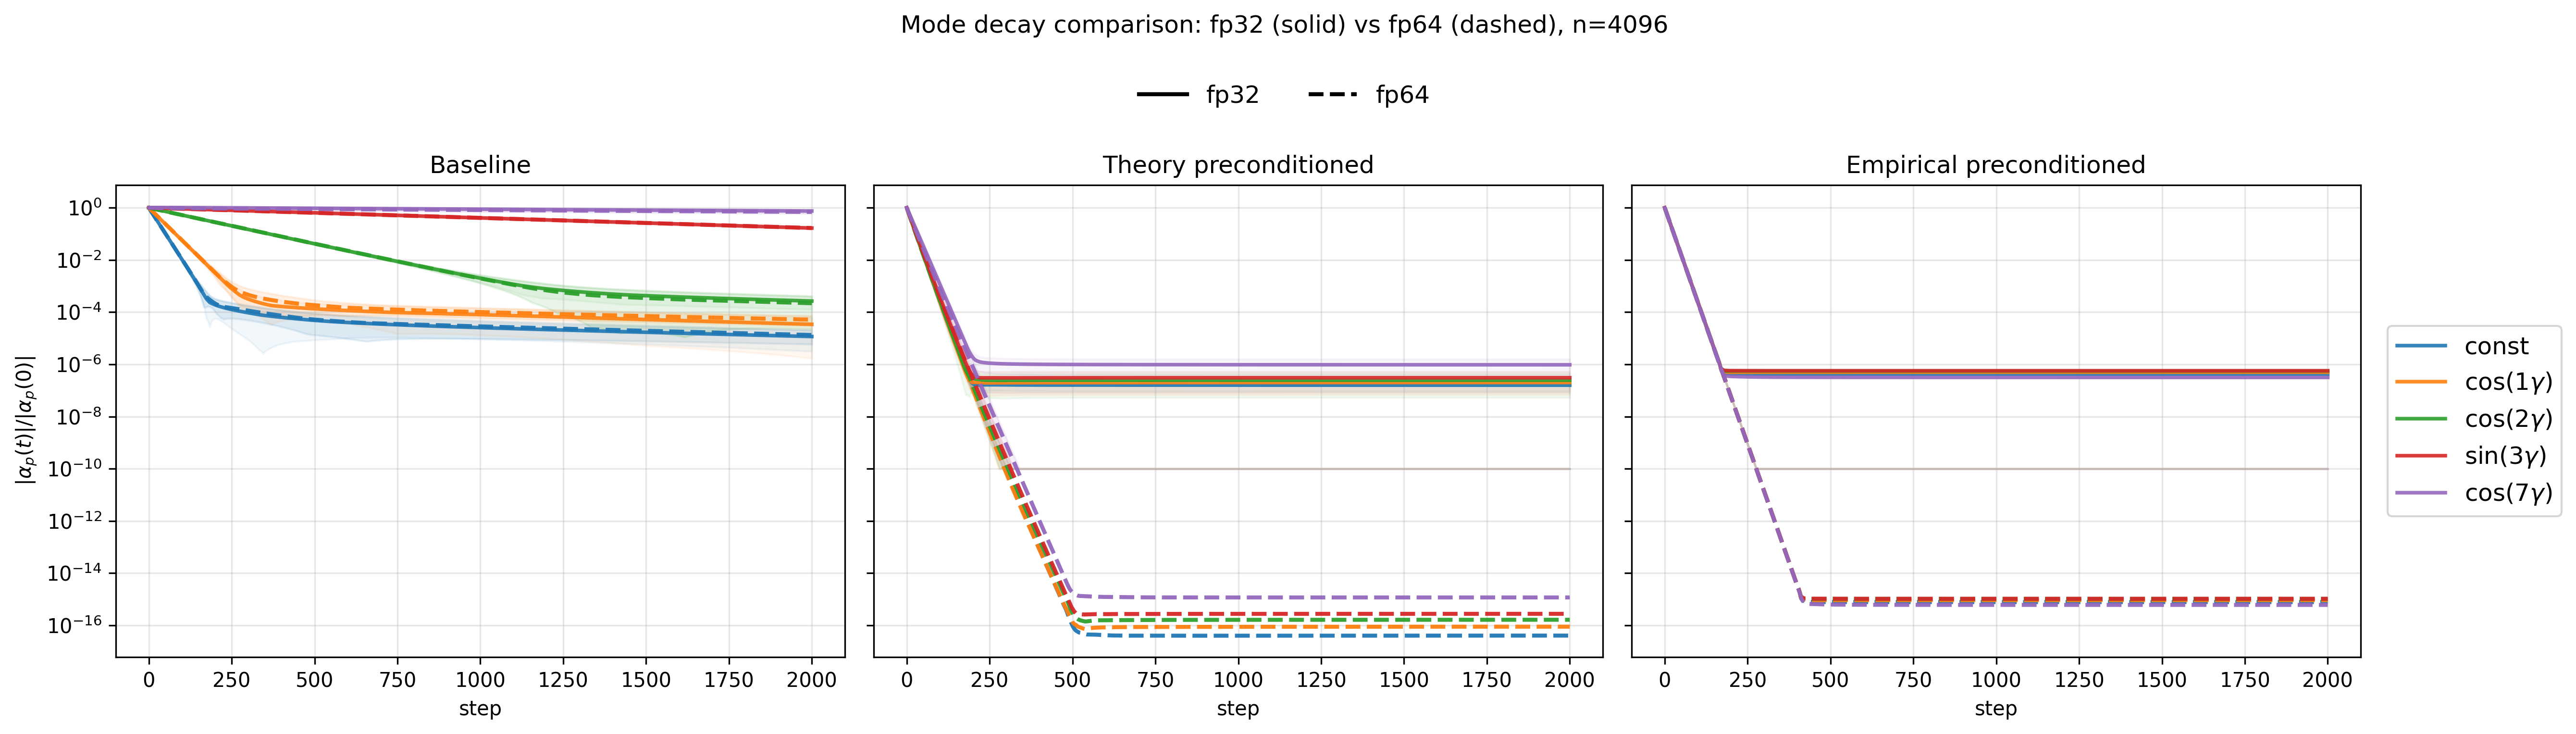
\includegraphics[width=\textwidth]{images/finite_sample_results/mode_decay_fp32_vs_fp64_three_panel_mean_std_n4096.png}
	\caption{Mode decay at \(n=4096\) in single (solid) and double (dashed)
		precision, for the baseline, theory-preconditioned, and empirically
		preconditioned dynamics. The preconditioned plateaus drop by several orders of
		magnitude from fp32 to fp64, identifying them as a finite-precision floor.}
	\label{fig:results-precision-comparison}
\end{figure}

\subsection{Targets with out-of-block frequencies}
\label{subsec:results-preconditioned-out-of-block}

The experiments so far kept all active target frequencies inside the retained
block. Figure~\ref{fig:results-precond-out-of-block} repeats the comparison with
a target that also contains frequencies outside the block, \(\sin(10\gamma)\) and
\(\cos(12\gamma)\). The preconditioner is still built only on the retained block,
so it accelerates the in-block modes as before but leaves the out-of-block modes
near their initial amplitude.

The in-block modes also plateau higher than in
Figure~\ref{fig:results-preconditioned-mode-decay}. This floor is not numerical:
the single- and double-precision curves reach nearly the same plateaus, so
roundoff is ruled out. We expect the cause to be coupling from the out-of-block
components. The sampled Fourier modes are only approximate eigenvectors of the
sampled operator, so the uncorrected modes at \(k=10\) and \(k=12\) can feed back
into the retained coordinates, and the in-block residuals would then settle at a
level set by this coupling. We have not isolated this mechanism directly, but it
is consistent with the modes being only approximate eigenvectors and with the
precision comparison ruling out roundoff.

\begin{figure}[!htbp]
	\centering
	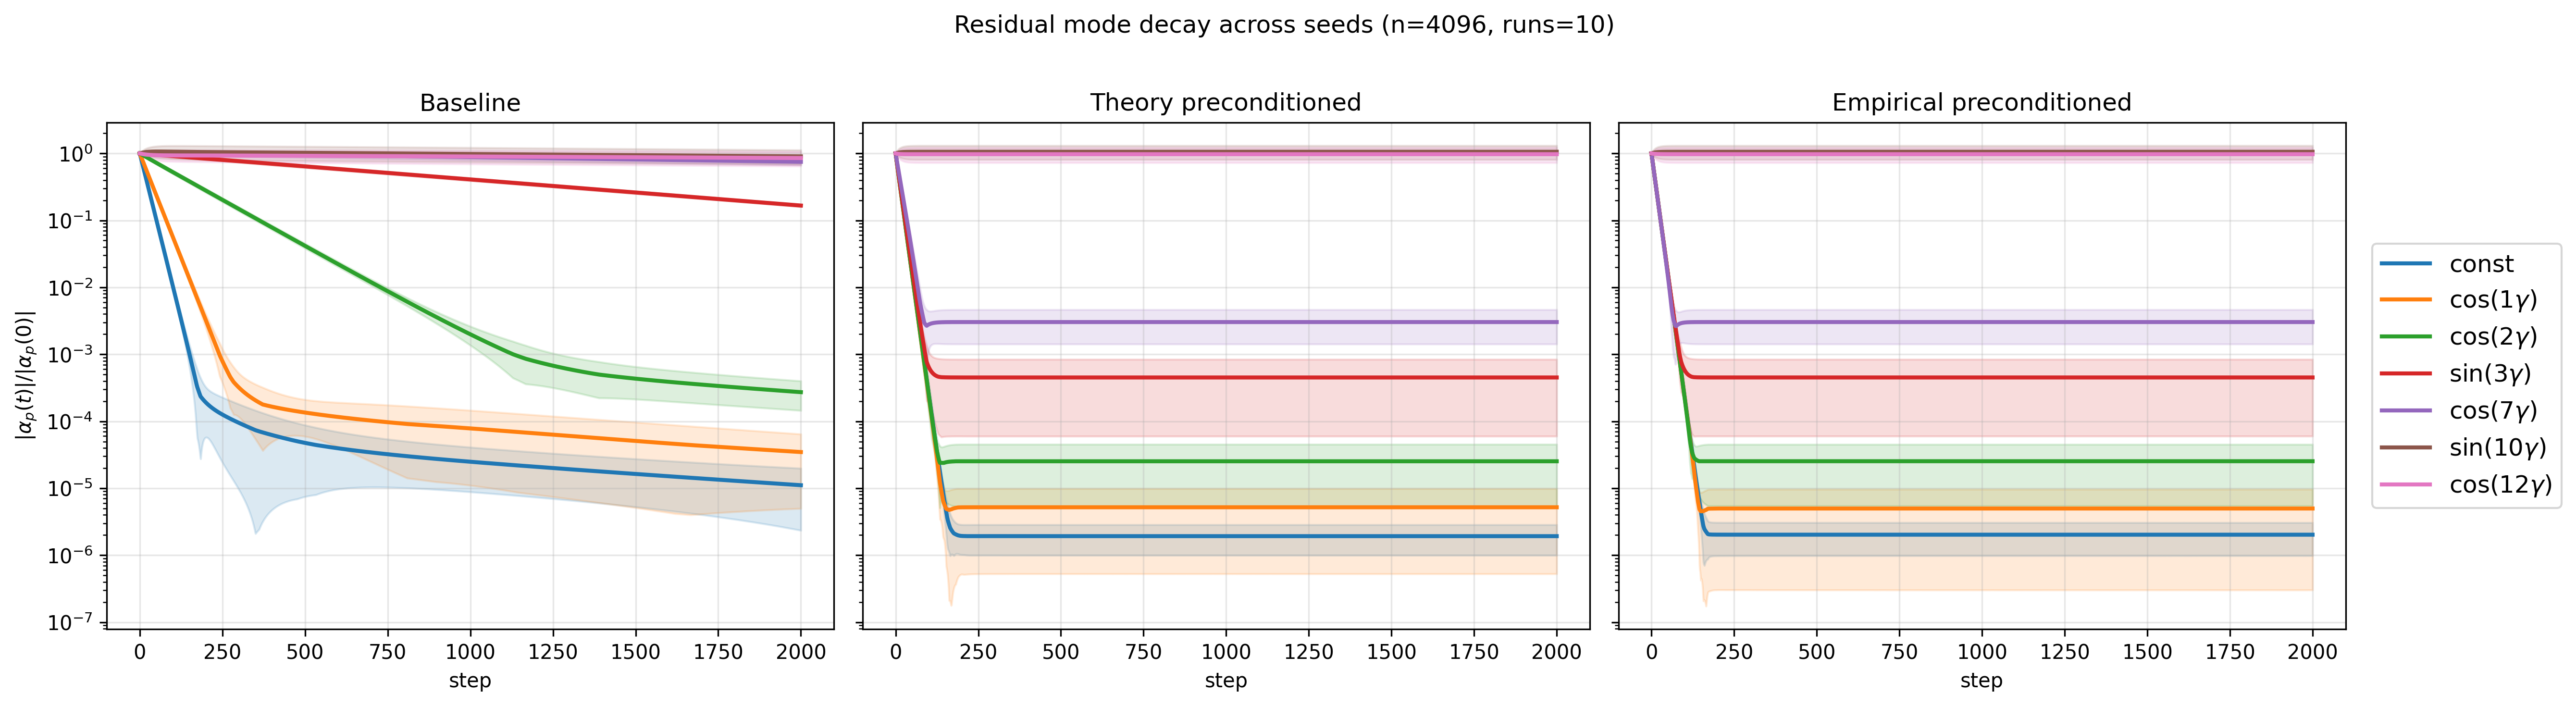
\includegraphics[width=\textwidth]{images/finite_sample_results/out_of_block_all_mode_decay_three_panel_mean_std_n4096.png}
	\caption{Preconditioned sampled dynamics with target frequencies outside the
		retained block, \(\sin(10\gamma)\) and \(\cos(12\gamma)\), at \(n=4096\) over
		\(10\) runs. The preconditioner accelerates the in-block modes but leaves the
		out-of-block modes near their initial amplitude. The in-block plateaus are
		higher than when all target modes lie inside the block, reflecting coupling
		from the uncorrected out-of-block components.}
	\label{fig:results-precond-out-of-block}
\end{figure}

\subsection{Discussion}
\label{subsec:results-preconditioned-discussion}

The preconditioning results connect to existing work on modifying NTK training
dynamics by changing the effective kernel spectrum. In particular,
\citet{geifman2024controlling} use preconditioned gradient descent to alter the
trajectory of wide-network training by modifying the spectrum of the associated
kernel. Recent work also studies preconditioned methods as a way to reduce
spectral bias and accelerate exploration of the NTK space
\citep{jiang2026convergencepreconditioned, yang2024sharpgeneralization}. Our
setting is more limited, since the preconditioner acts only on a fixed retained
Fourier block. The advantage is that the effect is explicit: rescaling by the
predicted eigenvalues directly compensates for the different decay rates of the
retained modes.

A practical use of this observation is as a block-level correction when the
target is known, or assumed, to be concentrated on a prescribed low-frequency
Fourier range. In that case, the theory preconditioner does not require
estimating the full sampled block inverse. It only uses the predicted
finite-sample eigenvalues \(\lambda_p^{(n)}\), and can make the retained
components converge on more similar time scales. The empirical preconditioner
gives the best correction when the sampled block is available, while the theory
preconditioner provides a cheaper approximation whose accuracy improves as the
finite-sample Fourier block becomes closer to diagonal.

Overall, the finite-sample results show that random sampling turns the exact
continuum Fourier dynamics into an approximate low-frequency description. The
sampled operator is no longer exactly diagonal in the Fourier basis, but its
deviation from the corrected diagonal prediction decreases with \(n\) and
explains the observed residual dynamics.

So far, however, the kernel itself has still been the deterministic
infinite-width NTK. In an actual finite-width network, the tangent kernel at
initialization is built from randomly initialized weights, so even before
training it is a random finite-width approximation of the continuum kernel. The
next section therefore asks whether the same Fourier structure survives this
second perturbation: finite width.

\section{Finite-width control of the frozen tangent operator}
\label{sec:results-finite-width-frozen}

We now turn from sampling error to width-induced error. Throughout this section, the input
space remains the continuum \(S^1\), and the object of interest is the frozen finite-width
operator \(B_m^{(K)}\) on the truncated Fourier subspace \(\mathcal H_K\), introduced in
\eqref{eq:method-finite-width-block}. The corresponding continuum reference block
\(\Lambda_K\) was defined in \eqref{eq:method-continuum-fourier-block}.

The next theorem shows that, for each fixed \(K\), the frozen finite-width block is a
controlled perturbation of the continuum Fourier block.

\begin{theorem}[Finite-width concentration of the frozen low-mode operator]
	\label{thm:results-finite-width-frozen-concentration}
	Fix \(K\ge 1\), and let \(d=2K+1\). Then
	\begin{equation}
		\mathbb E[B_m^{(K)}]=\Lambda_K.
		\label{eq:results-finite-width-mean}
	\end{equation}
	Moreover, there exists a universal constant \(c>0\) such that, for every
	\(\varepsilon>0\),
	\begin{equation}
		\mathbb P\!\left(
		\|B_m^{(K)}-\Lambda_K\|_{\max}\ge \varepsilon
		\right)
		\le
		2d^2
		\exp\!\left(
		-cm\min\!\left(\frac{\varepsilon^2}{32^2},\frac{\varepsilon}{32}\right)
		\right).
		\label{eq:results-finite-width-max-bound}
	\end{equation}
	Equivalently, for every \(\delta\in(0,1)\), with probability at least
	\(1-\delta\),
	\begin{equation}
		\|B_m^{(K)}-\Lambda_K\|_{\max}
		\le
		32\max\left\{
		\sqrt{\frac{1}{cm}\log\!\left(\frac{2d^2}{\delta}\right)},
		\frac{1}{cm}\log\!\left(\frac{2d^2}{\delta}\right)
		\right\}.
		\label{eq:results-finite-width-high-prob-bound}
	\end{equation}
	In particular, for fixed \(K\),
	\begin{equation}
		\|B_m^{(K)}-\Lambda_K\|_{\max}
		=
		O \!\left(\sqrt{\frac{\log K}{m}}\right).
		\label{eq:results-finite-width-rate}
	\end{equation}
\end{theorem}

The detailed proof is provided in Appendix~\ref{app:finite-width-frozen-proofs}.

Theorem~\ref{thm:results-finite-width-frozen-concentration} shows that, on a
fixed truncated Fourier subspace, the frozen finite-width tangent block is a
random perturbation of the continuum Fourier block. The perturbation decreases
with width at the usual \(m^{-1/2}\) concentration scale, up to logarithmic
factors in the block dimension. However, the theorem contains an unspecified
universal constant \(c>0\). This constant comes from Bernstein's inequality for
averages of centered sub-exponential random variables
\citep{Vershynin_2018a}. In explicit proofs of such inequalities, constants of
order \(1/4\) often appear after converting a \(\psi_1\)-norm bound into a
moment generating function bound. We next check this concentration behavior numerically where
we use \(c=0.2\) as a conservative
representative value, not an optimized constant for this problem. Changing this
constant shifts the bound but does not change the predicted rate as \(m\) increases.

For each width \(m\), we sample 100 independent initializations and compute
\[
	\|B_m^{(K)}-\Lambda_K\|_{\max}.
\]
Figure~\ref{fig:results-finite-width-concentration} shows the median and
\(95\%\) quantile of this error, together with the rate envelope suggested by
Theorem~\ref{thm:results-finite-width-frozen-concentration}.
The empirical errors decrease steadily with width. The theoretical envelope is
much larger than the observed errors, but it has the correct qualitative trend:
the finite-width block concentrates around the continuum Fourier block as \(m\)
increases.

\begin{figure}[!htbp]
	\centering
	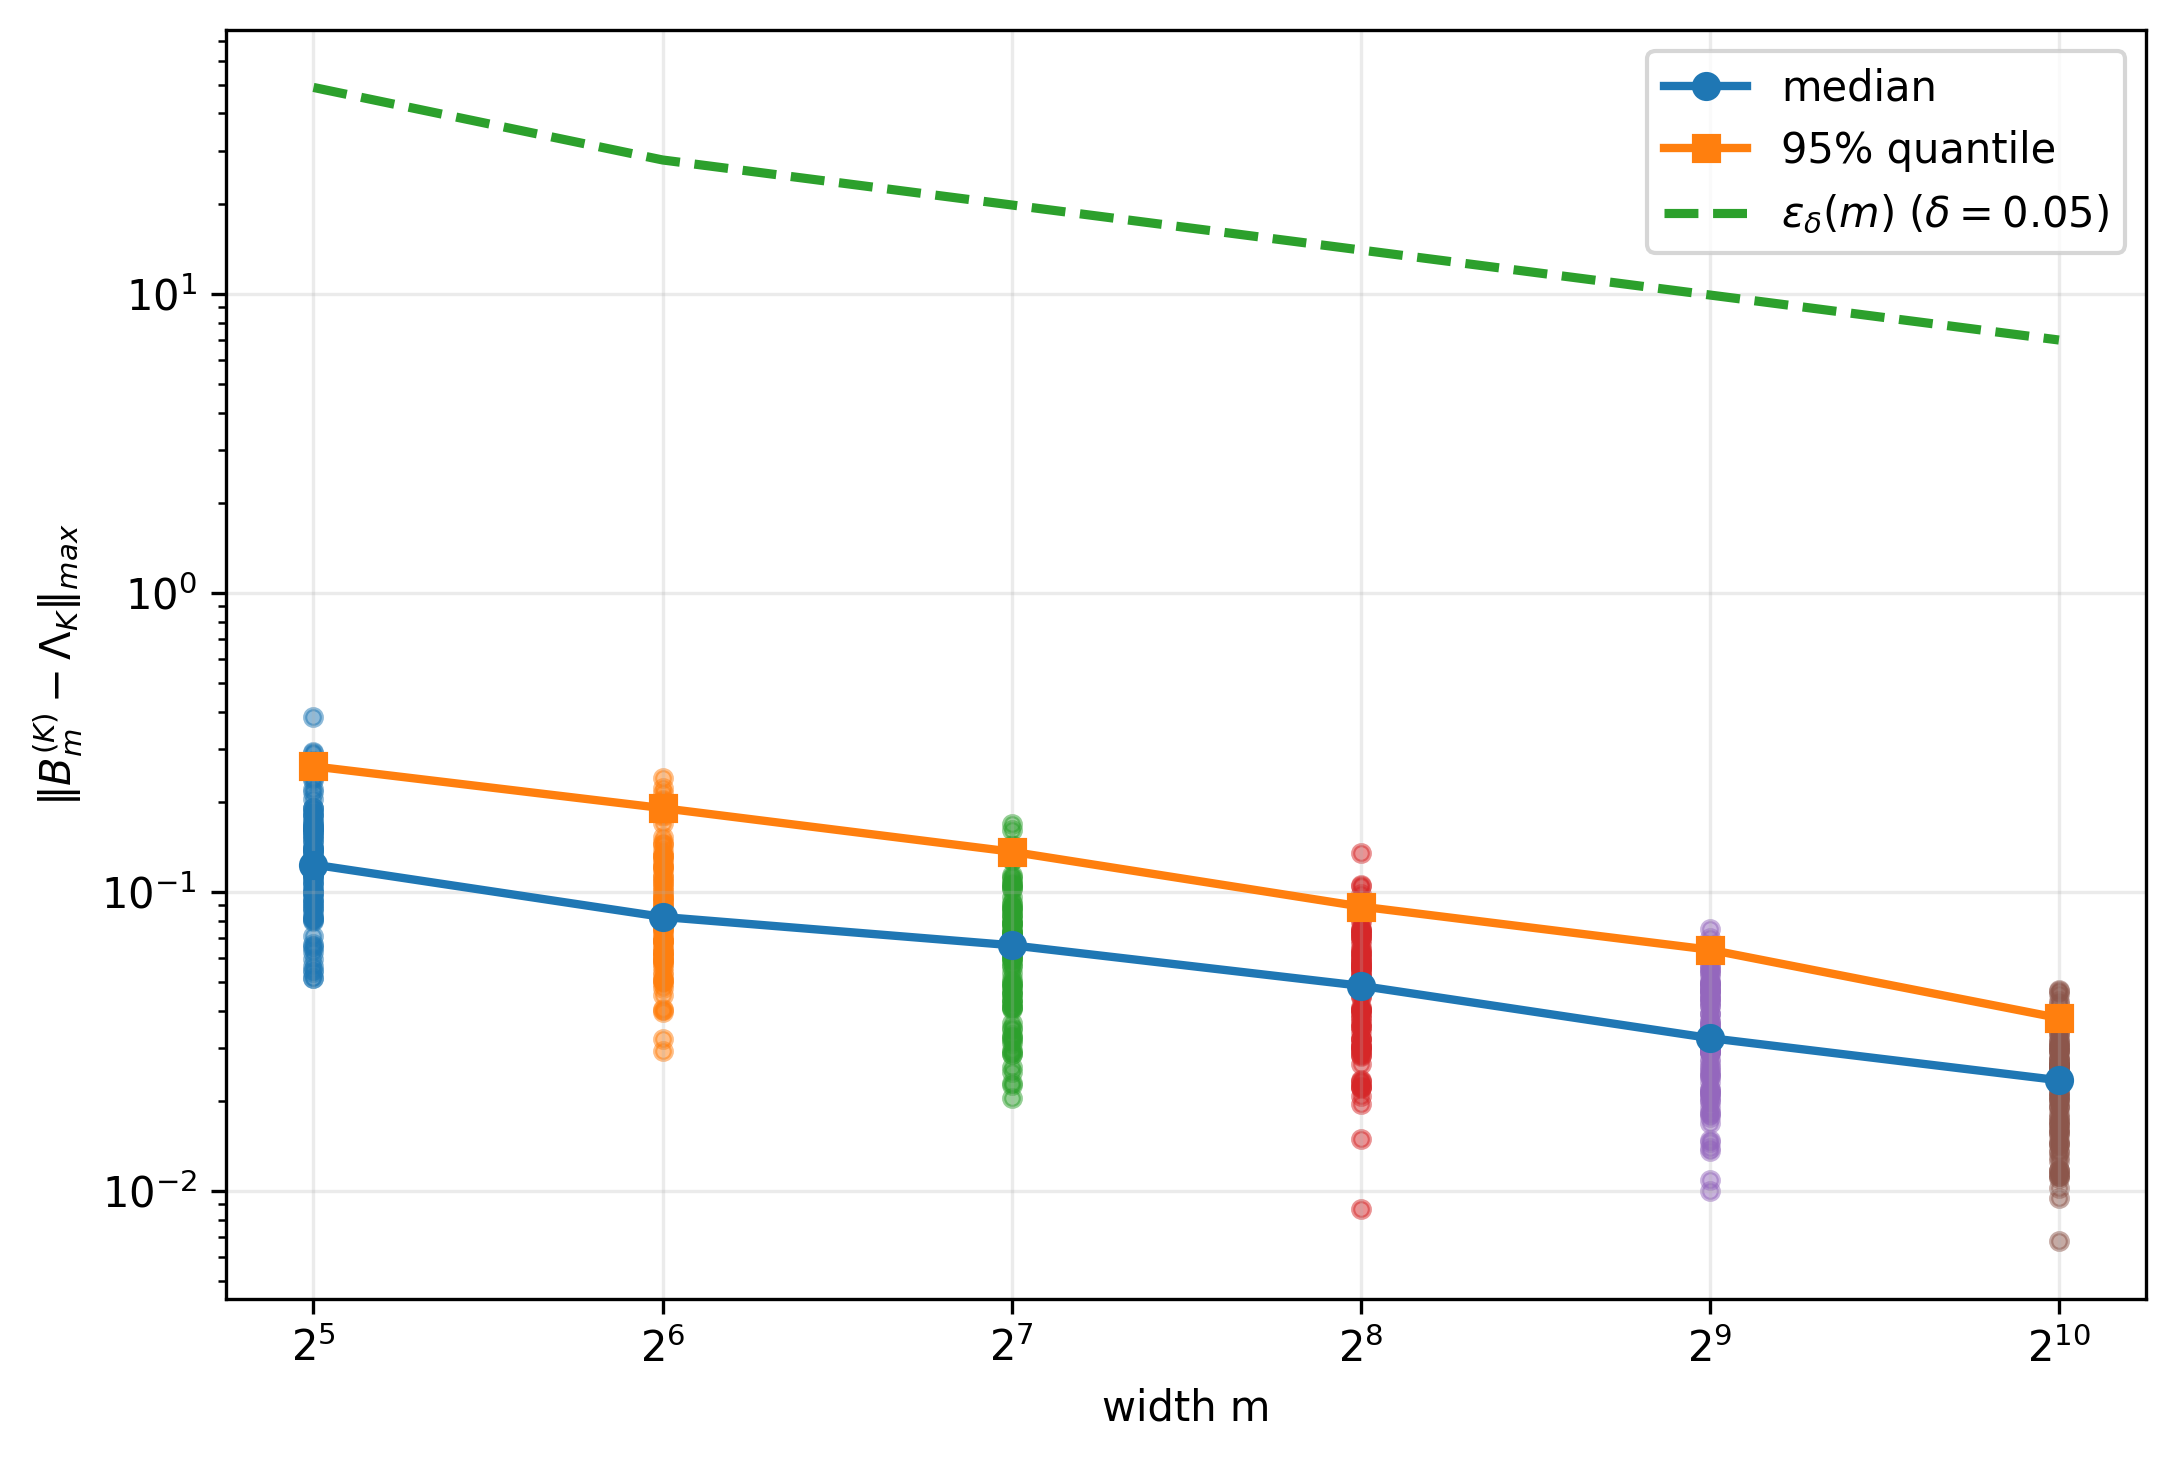
\includegraphics[width=0.82\textwidth]{images/finite_width_results/03_concentration_B_m.png}
	\caption{Finite-width concentration of the frozen tangent block. For each
	width \(m\), the plot shows the median and \(95\%\) quantile of
	\(\|B_m^{(K)}-\Lambda_K\|_{\max}\) across 100 independent initializations. The
	dashed curve shows the rate envelope from
	Theorem~\ref{thm:results-finite-width-frozen-concentration} with
	\(\delta=0.05\) and the illustrative constant \(c=0.2\). The empirical errors
	decrease with width, while the explicit envelope is conservative.}
	\label{fig:results-finite-width-concentration}
\end{figure}

This is the finite-width analogue of the finite-sample
control from the previous section. In the finite-sample case, the randomness
comes from replacing the uniform measure by sampled points. Here, the randomness
comes from the finite number of hidden units at initialization. In both cases,
on a fixed low-frequency Fourier block, the
operator remains close to the deterministic continuum Fourier block, and the
deviation decreases as the relevant size parameter (number of samples or width of network) increases.

Thus finite width alone does not destroy the Fourier structure of the frozen
tangent operator. For a particular random initialization, the operator is not
exactly diagonal in the Fourier basis, but
Theorem~\ref{thm:results-finite-width-frozen-concentration} and
Figure~\ref{fig:results-finite-width-concentration} show that this mismatch
shrinks with width. This supports the use of the infinite-width NTK as a
baseline, while also showing why finite-width fluctuations can matter
quantitatively
\citep{jacot2018ntk,lee2020wide,bordelon2023dynamicsfinitewidthkernel,
	vyas2022limitationsntkunderstandinggeneralization}.

The next question is whether this entrywise concentration also corresponds to
geometric agreement of the frequency subspaces themselves.

\subsection{Empirical alignment of Fourier frequency subspaces}
\label{subsec:results-finite-width-subspace-alignment}

The block concentration result controls the matrix \(B_m^{(K)}\) on the retained
Fourier coordinates. We next examine the corresponding eigenspaces directly.
Using the quantities introduced in
Section~\ref{subsec:method-projector-error}, we compare each Fourier frequency
subspace \(\mathcal F_k\) with a matched empirical eigenspace
\(\widehat{\mathcal F}_k\) of the frozen finite-width operator.

We first summarize the comparison using the projector error
\[
	\varepsilon_{k,F}^{(m)}
	=
	\|\widehat P_k-P_k\|_F .
\]
This gives one scalar mismatch measure for each frequency subspace. By
\eqref{eq:method-projector-angle-identity}, it is equivalent to combining the
principal angles between \(\mathcal F_k\) and \(\widehat{\mathcal F}_k\).

Figure~\ref{fig:results-finite-width-projector-error} shows the mean and
standard deviation of \(\varepsilon_{k,F}\) across random initializations.
For all displayed frequencies, the projector error decreases as the width
increases. Higher frequencies generally have larger projector error at a fixed
width. One exception in this experiment is \(k=2\), which has the smallest
projector error among the displayed frequencies.
A plausible explanation is the structural role of
\(k=0\) and \(k=1\) in this chosen architecture.
The constant mode receives a direct eigenvalue contribution from the trainable
hidden-bias term (refer Theorem~\ref{thm:results-continuum-spectrum}).
The first frequency, \(k=1\), is tied to the coordinate embedding,
\[
	x(\varphi)=(\cos\varphi,\sin\varphi)
\]
and it is also the only odd frequency
present in the no-bias kernel (Corollary~\ref{cor:results-bias-spectrum}), with

\[
	\lambda_1^{(\mathrm{nb})}=\frac14,
	\qquad
	\lambda_k^{(\mathrm{nb})}=0
	\quad \text{for odd } k\ge 3.
\]
These features may make the finite-width perturbation act differently on \(k=0\) and \(k=1\) than on the
higher frequency blocks. We do not investigate this mechanism further here, so
the \(k=2\) behavior is an empirical observation and not a theoretical claim.

\begin{figure}[!htbp]
	\centering
	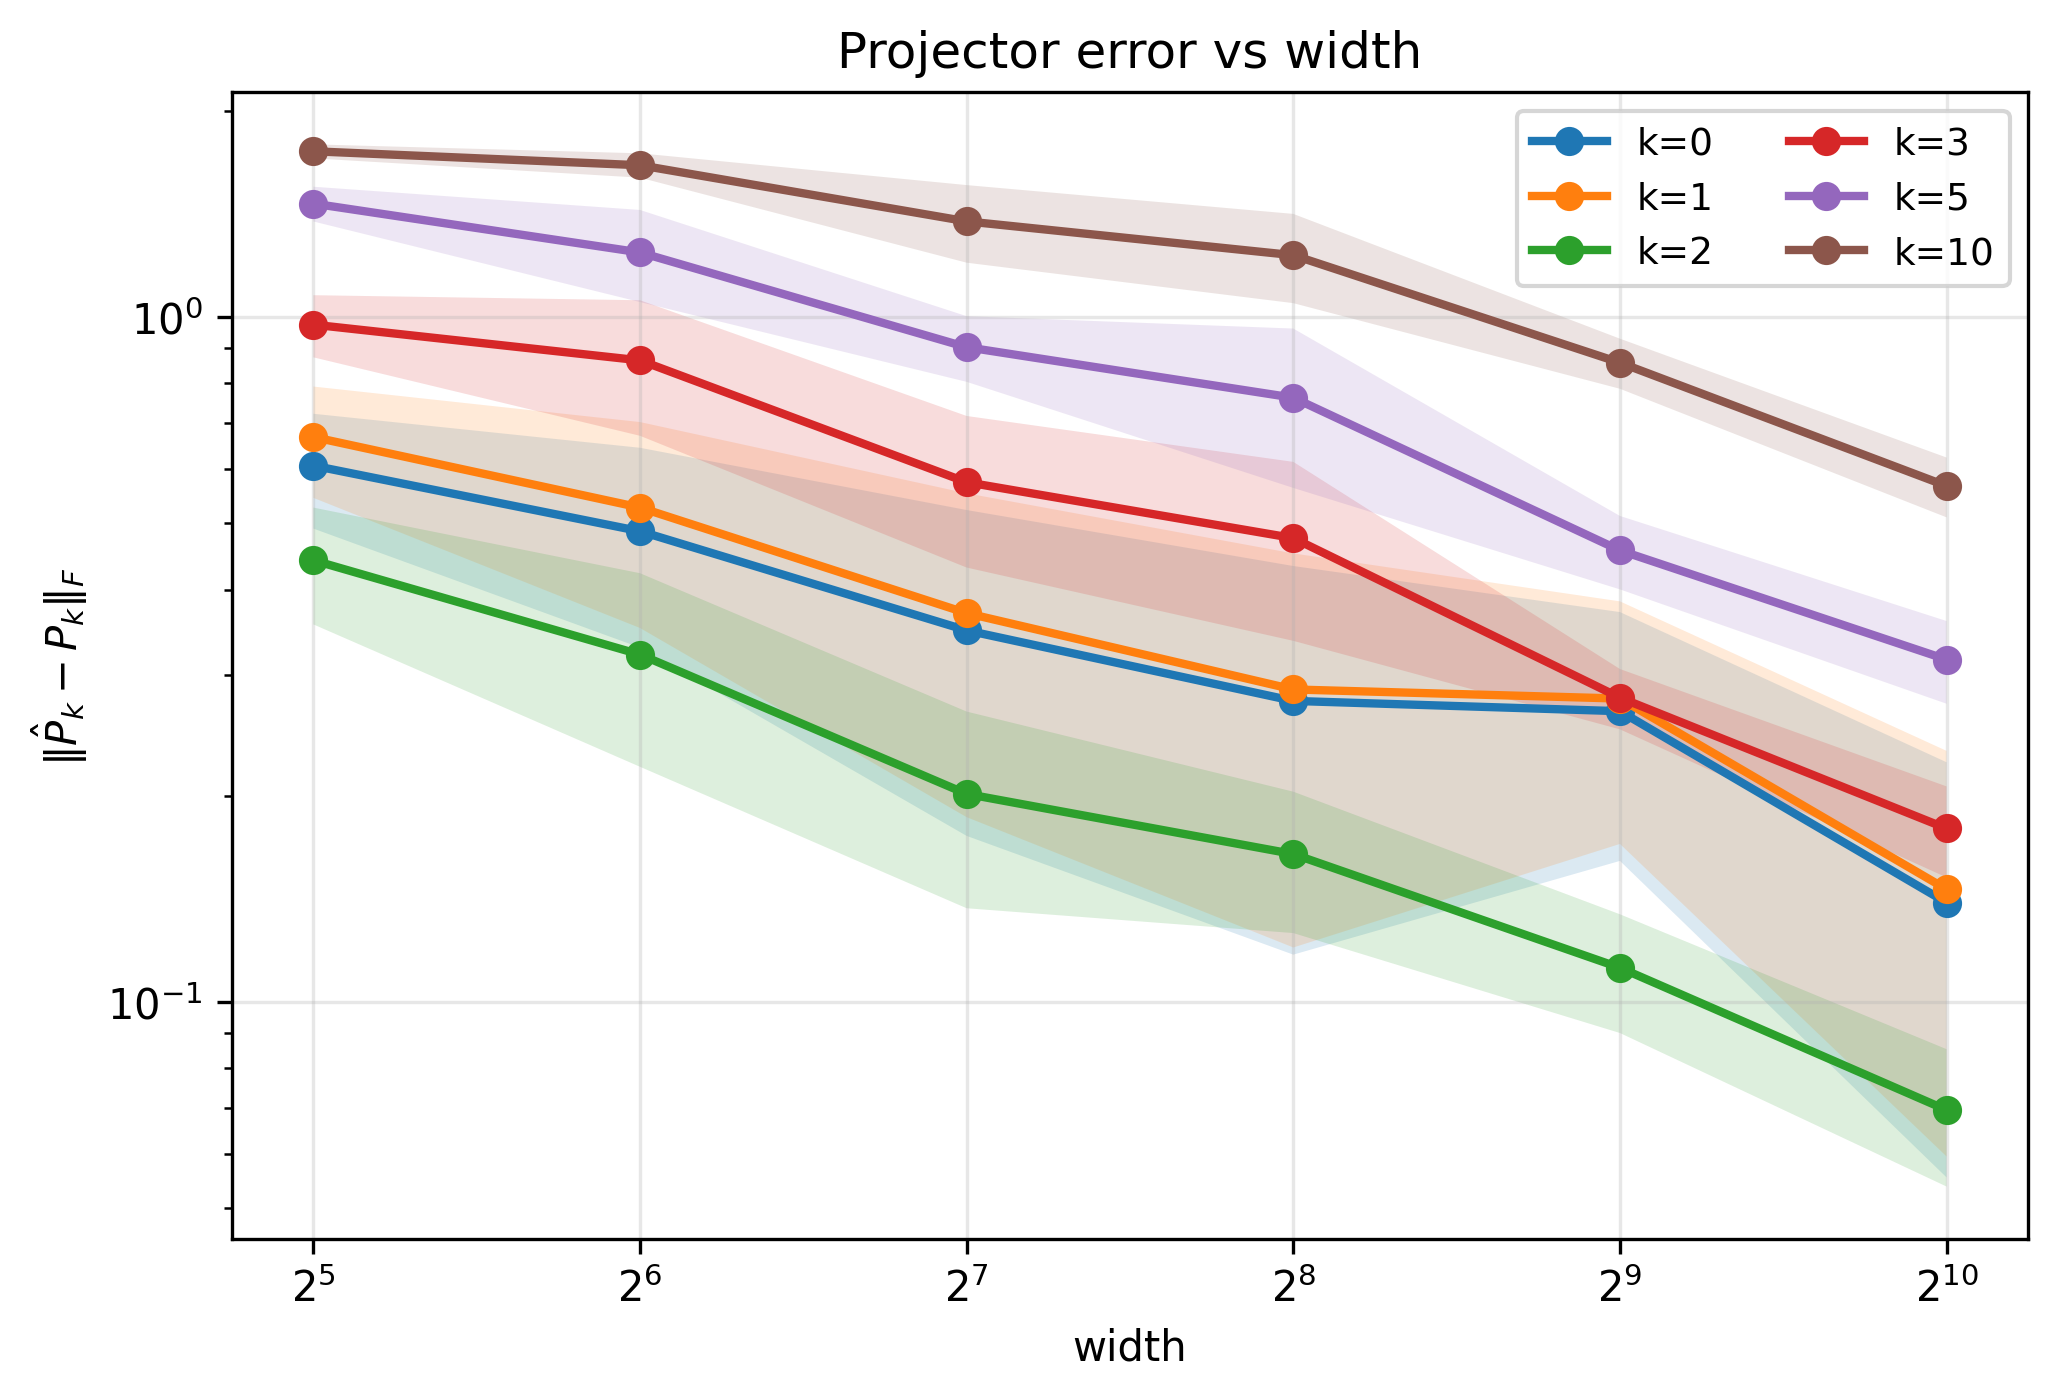
\includegraphics[width=0.78\textwidth]{images/finite_width_results/projector_error_vs_width.png}
	\caption{Projector error
		\(\|\widehat P_k-P_k\|_F\) between the Fourier frequency subspace
		\(\mathcal F_k\) and the matched empirical eigenspace
		\(\widehat{\mathcal F}_k\) of the frozen finite-width operator at
		initialization. The markers show the mean over random initializations and the
		shaded regions show one standard deviation. The error decreases with width
		for all displayed frequencies.}
	\label{fig:results-finite-width-projector-error}
\end{figure}

The projector error gives one scalar measure of subspace mismatch. As a
complementary summary, we also report the subspace cosine similarity defined in
\eqref{eq:method-subspace-cosine-similarity}. This quantity averages the
squared cosines of the principal angles between \(\mathcal F_k\) and
\(\widehat{\mathcal F}_k\), and lies between \(0\) and \(1\). Larger values
indicate better alignment, with value \(1\) corresponding to perfect agreement
of the two subspaces.

Figure~\ref{fig:results-finite-width-subspace-cosine-similarity} shows this
alignment score across widths. The alignment improves with \(m\) for all
displayed frequencies, matching the trend in the projector-error plot. Lower
frequencies are already well aligned at small width, while higher frequencies
require larger widths to approach the continuum Fourier subspaces. As before,
\(k=2\) is unusually well aligned compared with neighbouring displayed
frequencies.

% \begin{figure}[H]
% 	\centering
% 	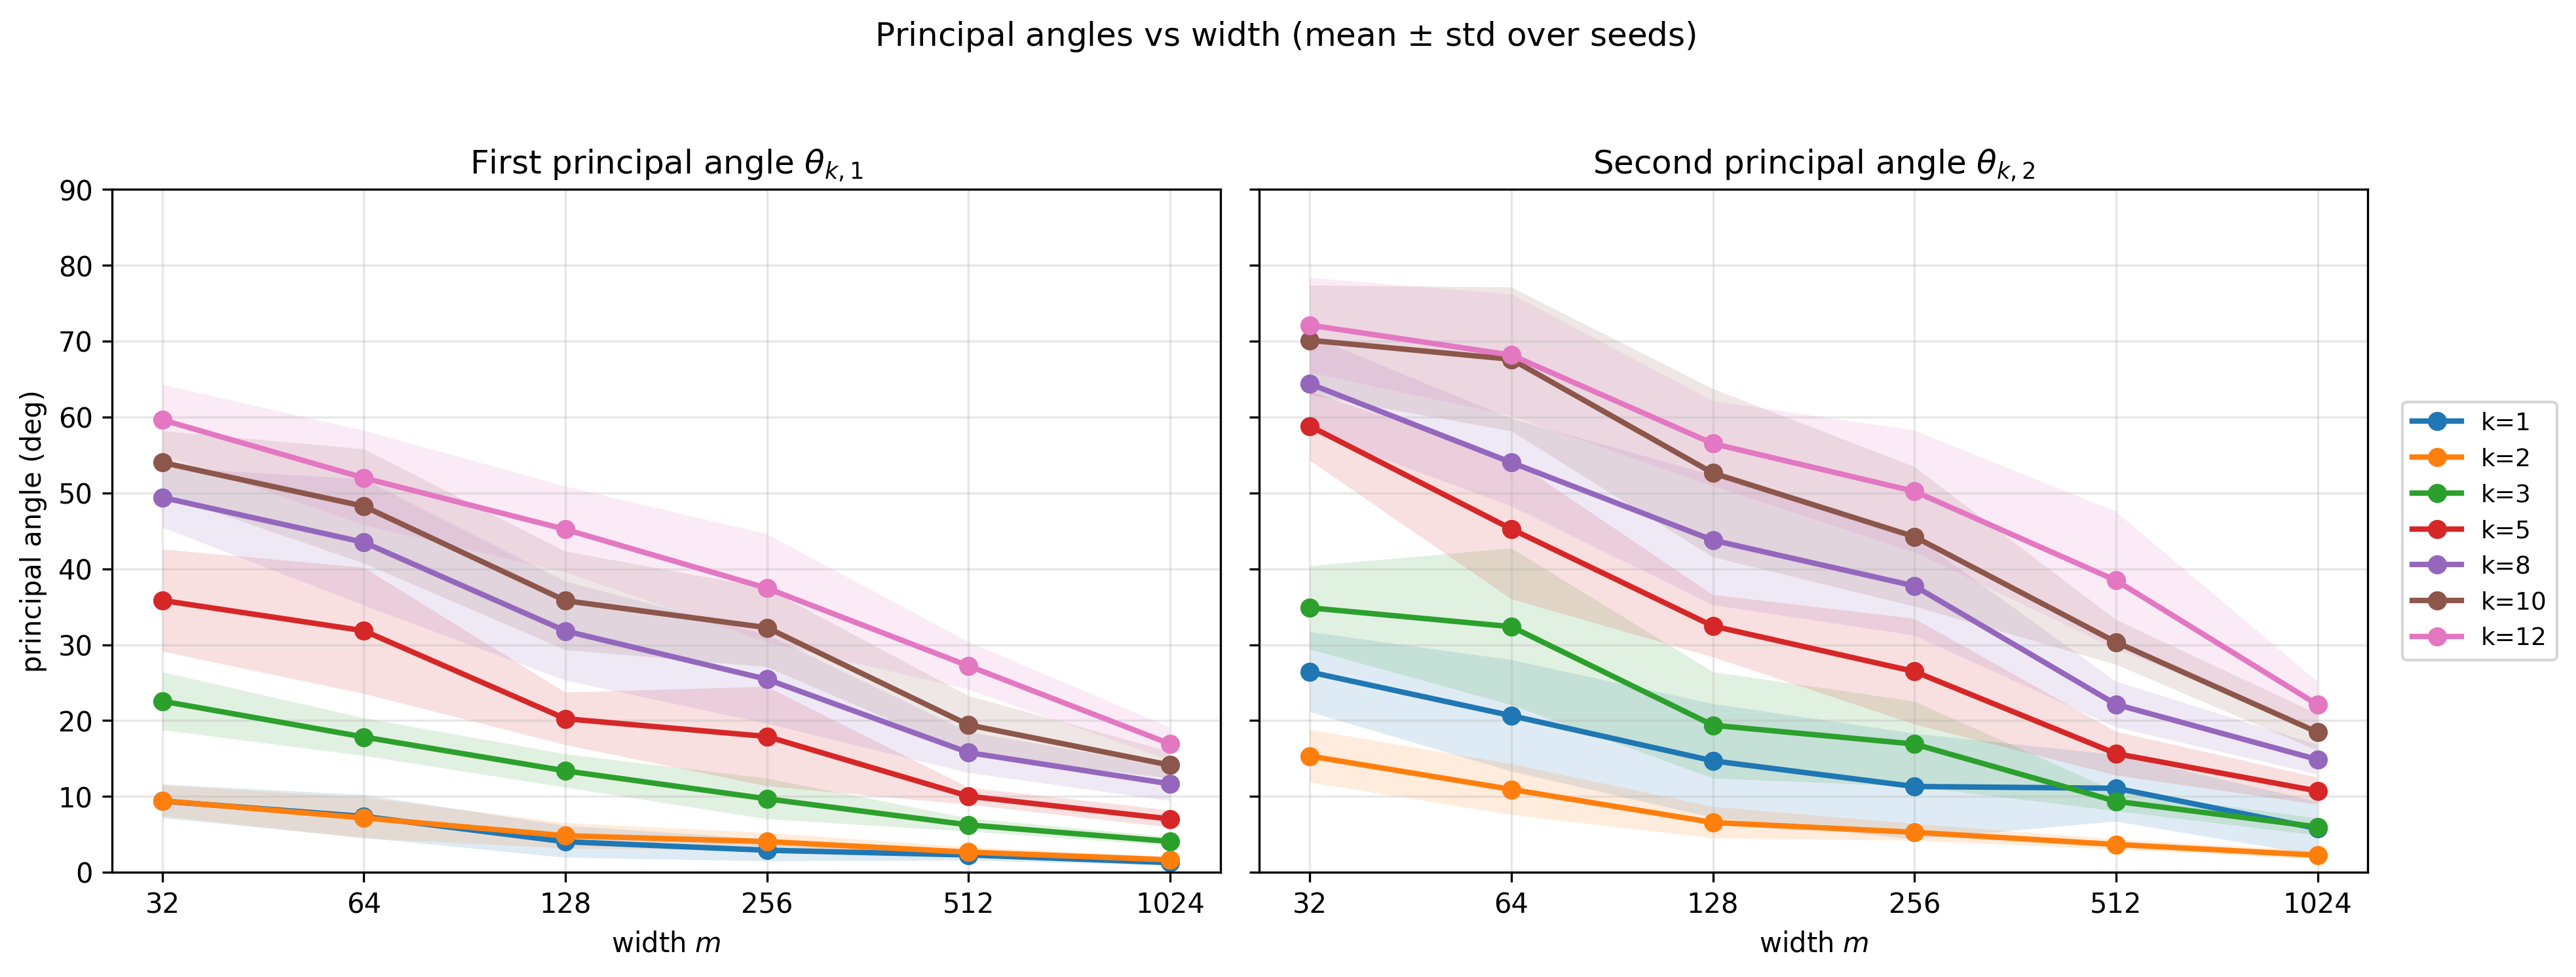
\includegraphics[width=\textwidth]{images/finite_width_results/principal_angles_vs_width.png}
% 	\caption{Principal angles between the Fourier frequency subspace
% 		\(\mathcal F_k\) and the matched empirical eigenspace
% 		\(\widehat{\mathcal F}_k\) of the frozen finite-width operator at
% 		initialization. The left panel shows the first principal angle
% 		\(\theta_{k,1}\), and the right panel shows the second principal angle
% 		\(\theta_{k,2}\). The markers show the mean over random initializations and
% 		the shaded regions show one standard deviation. The principal angles tend to
% 		decrease with width.}
% 	\label{fig:results-finite-width-principal-angles}
% \end{figure}

\begin{figure}[!htbp]
	\centering
	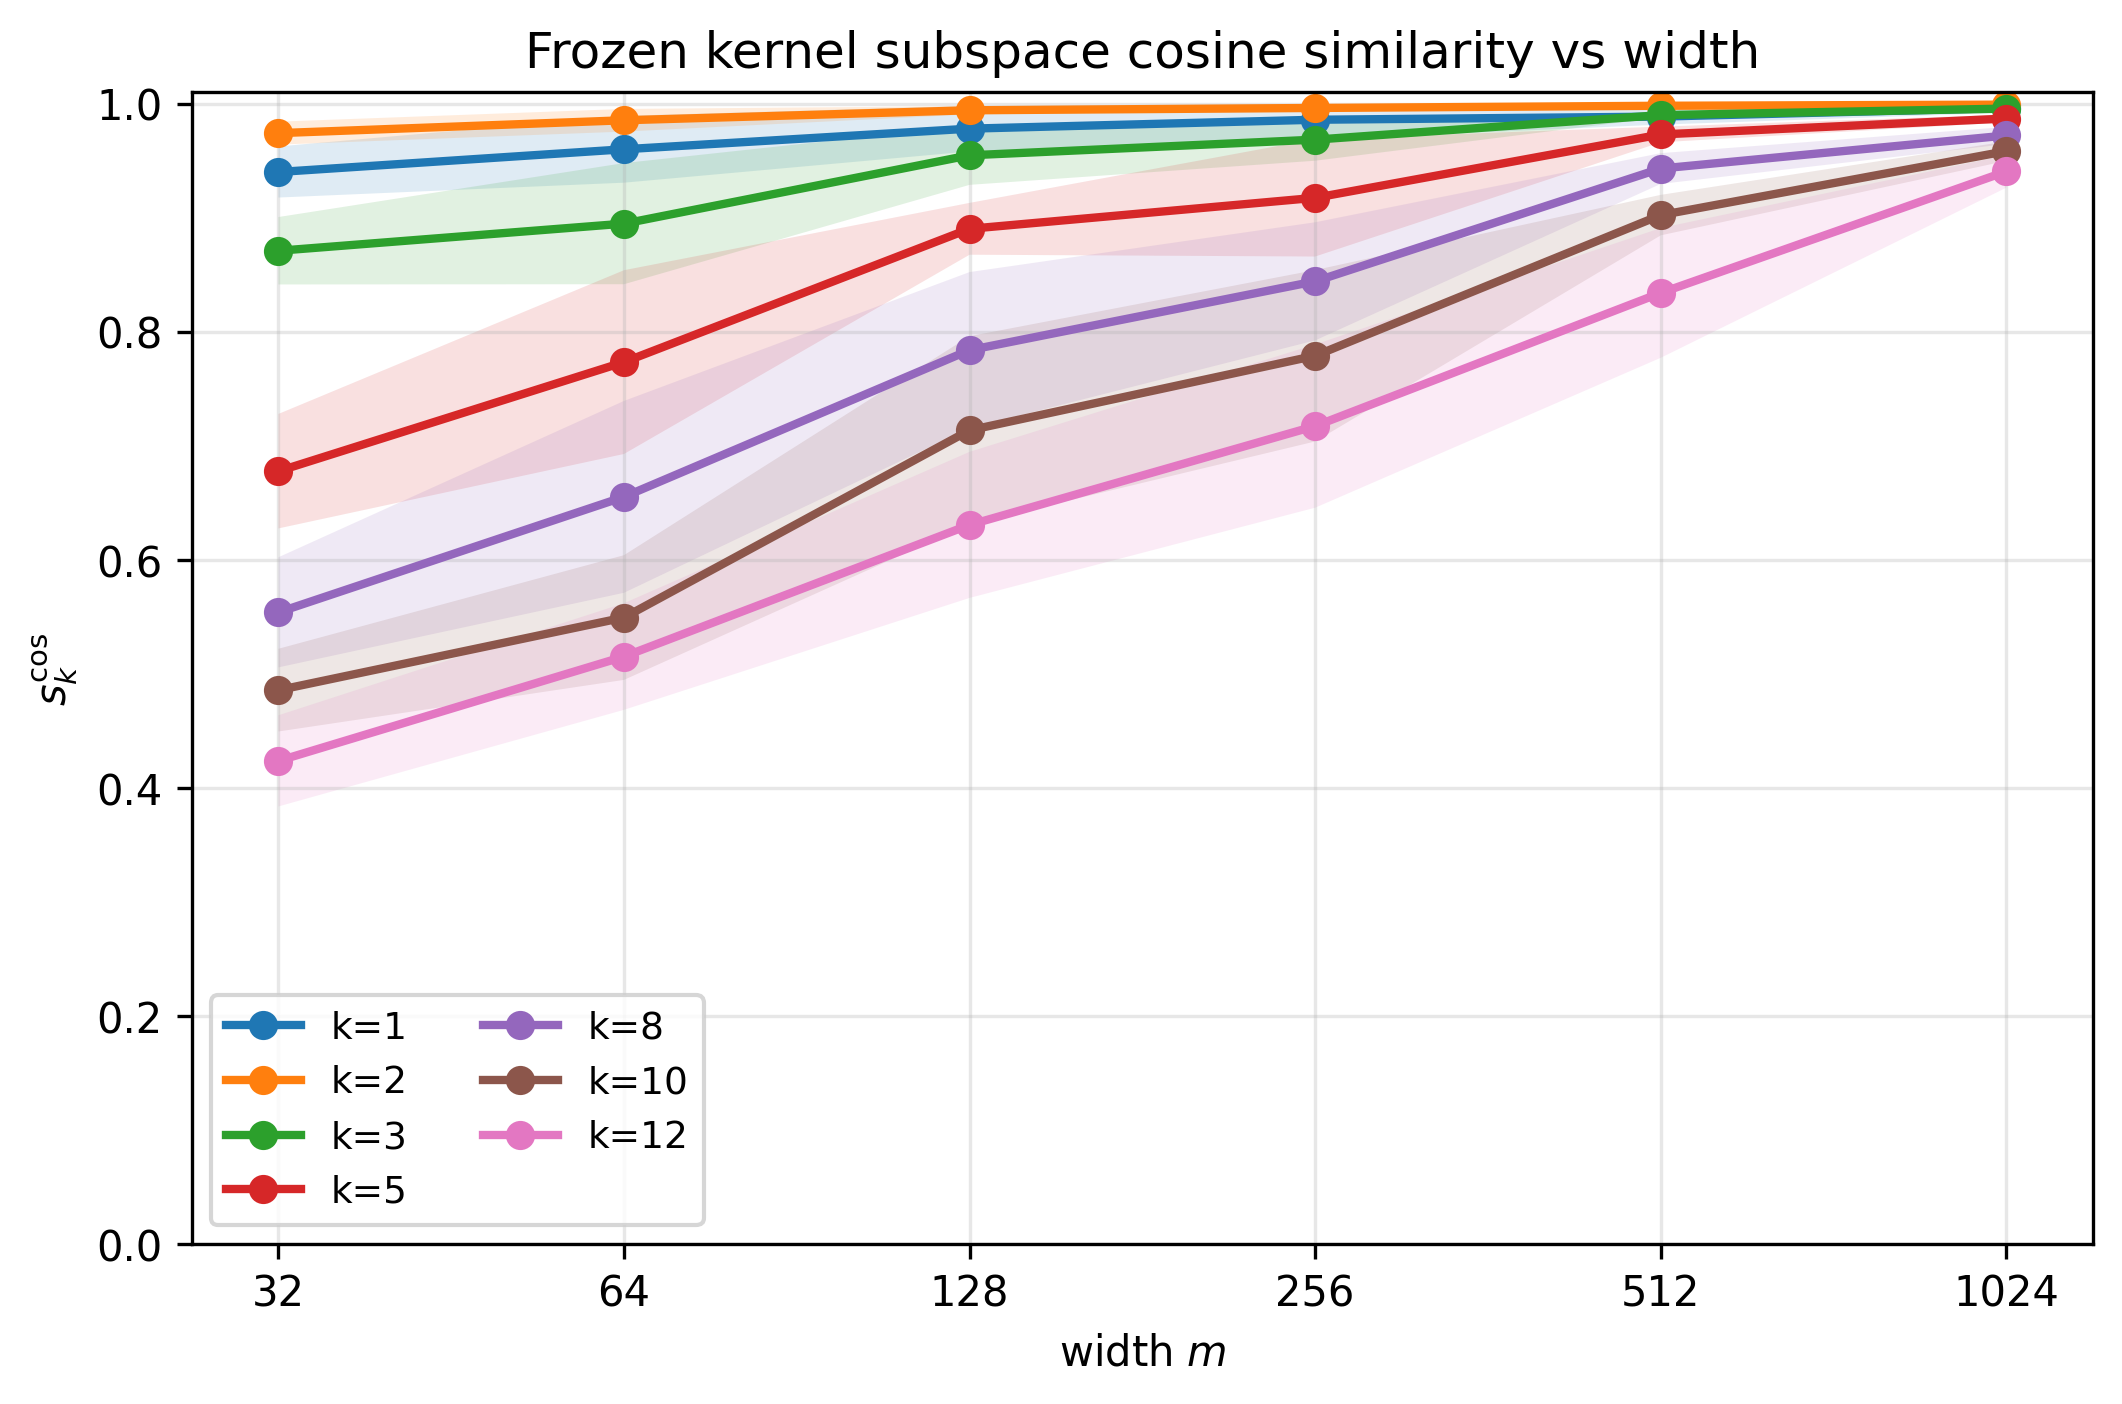
\includegraphics[width=0.78\textwidth]{images/finite_width_results/rms_cos_similarity_vs_width.png}
	\caption{Subspace cosine similarity between the Fourier frequency subspace
		\(\mathcal F_k\) and the matched empirical eigenspace
		\(\widehat{\mathcal F}_k\) of the frozen finite-width operator at
		initialization. The markers show the mean over random initializations and
		the shaded regions show one standard deviation. Larger values indicate
		better subspace alignment, with value \(1\) corresponding to perfect
		alignment. The alignment improves with width for all displayed frequencies,
		with higher frequencies requiring larger widths to approach the continuum
		Fourier subspaces.}
	\label{fig:results-finite-width-subspace-cosine-similarity}
\end{figure}

Taken together, Figures~\ref{fig:results-finite-width-concentration},
\ref{fig:results-finite-width-projector-error}, and
\ref{fig:results-finite-width-subspace-cosine-similarity} show the same finite-width
trend from complementary viewpoints. The matrix block \(B_m^{(K)}\) approaches
the continuum block \(\Lambda_K\) as \(m\) increases, and the matched empirical
eigenspaces become closer to the corresponding Fourier frequency subspaces.
The improvement is strongest at small and moderate widths for the higher
frequencies, which are the most poorly aligned at small width.

The concentration theorem controls the absolute error
\(|B_m^{(K)}-\Lambda_K|_{\max}\). To interpret its effect on a particular
Fourier component, this error should be compared with the size of the
corresponding continuum eigenvalue. In the continuum fixed-kernel model, mode
\(k\) decays at rate \(\lambda_k\), and
Theorem~\ref{thm:results-continuum-spectrum} gives
\[
	\lambda_k = O(k^{-2})
	\qquad (k\to\infty),
\]
for both even and odd frequencies. Thus, the same absolute perturbation is less
important for low-frequency modes with larger eigenvalues, and can be more
visible for high-frequency modes with smaller eigenvalues. This explains why the
finite-width perturbation is expected to matter more for higher frequencies.

Figures~\ref{fig:results-finite-width-subspace-cosine-similarity} and
\ref{fig:results-finite-width-projector-error}, support this interpretation
geometrically. For \(k \ge 1\), each Fourier frequency corresponds to a
two-dimensional plane spanned by the cosine and sine modes. At finite width,
the matched empirical eigenspace need not coincide exactly with this plane. The
projector-error and cosine-similarity plots show that this mismatch decreases
with width. They also show that the amount of alignment can vary substantially
across frequencies at the same width. One plausible explanation is that
eigenspace stability depends not only on the size of the finite-width
perturbation, but also on the local spectral separation of the corresponding
continuum eigenspace. Since higher-frequency eigenvalues are smaller and closer
together, their eigenspaces may be more sensitive to the same absolute
perturbation.

Overall, the frozen finite-width results show that finite width does not
destroy the Fourier structure at initialization. It introduces a random
perturbation of the continuum Fourier operator, and this perturbation decreases
with width. The result is, therefore, a frozen-kernel baseline: before training
changes the tangent operator, the continuum Fourier eigenspaces remain a useful
reference, but finite-width fluctuations can already affect higher-frequency
components more strongly. This is consistent with empirical observations that
higher-frequency components are learned later and are more sensitive to the
data distribution and to perturbations
\citep{rahaman2019spectralbiasneuralnetworks,basri2019convergence,basri2020frequencybiasneuralnetworks}.

The part not settled here is the evolving finite-width case. During training,
the tangent operator can change, so the frozen Fourier block structure need not
remain fixed. The finite-width result therefore gives us a
frozen-kernel baseline but not a complete theory of finite-width training
\citep{bordelon2023dynamicsfinitewidthkernel,vyas2022limitationsntkunderstandinggeneralization,golikov2022neuraltangentkernelsurvey}.

\section{Evolving finite-width tangent kernel}
\label{sec:results-evolving-kernel}

The previous section studied the frozen tangent operator at initialization. We
now compare this frozen baseline with the tangent operator that evolves during
training. Unlike the finite-width concentration result above, this part is
empirical. The goal is to understand how kernel evolution changes the Fourier
picture at finite width.

\subsection{Loss decay across widths}
\label{subsec:results-evolving-loss}

We first compare the least-squares objective under frozen and evolving
finite-width tangent-kernel dynamics across widths. The cross-width comparison
in Figure~\ref{fig:evolving-cross-width-loss} gives the overall trend, while
Figure~\ref{fig:evolving-loss-by-width} shows the width-by-width frozen versus
evolving comparison in more detail.

\begin{figure}[!htbp]
	\centering
	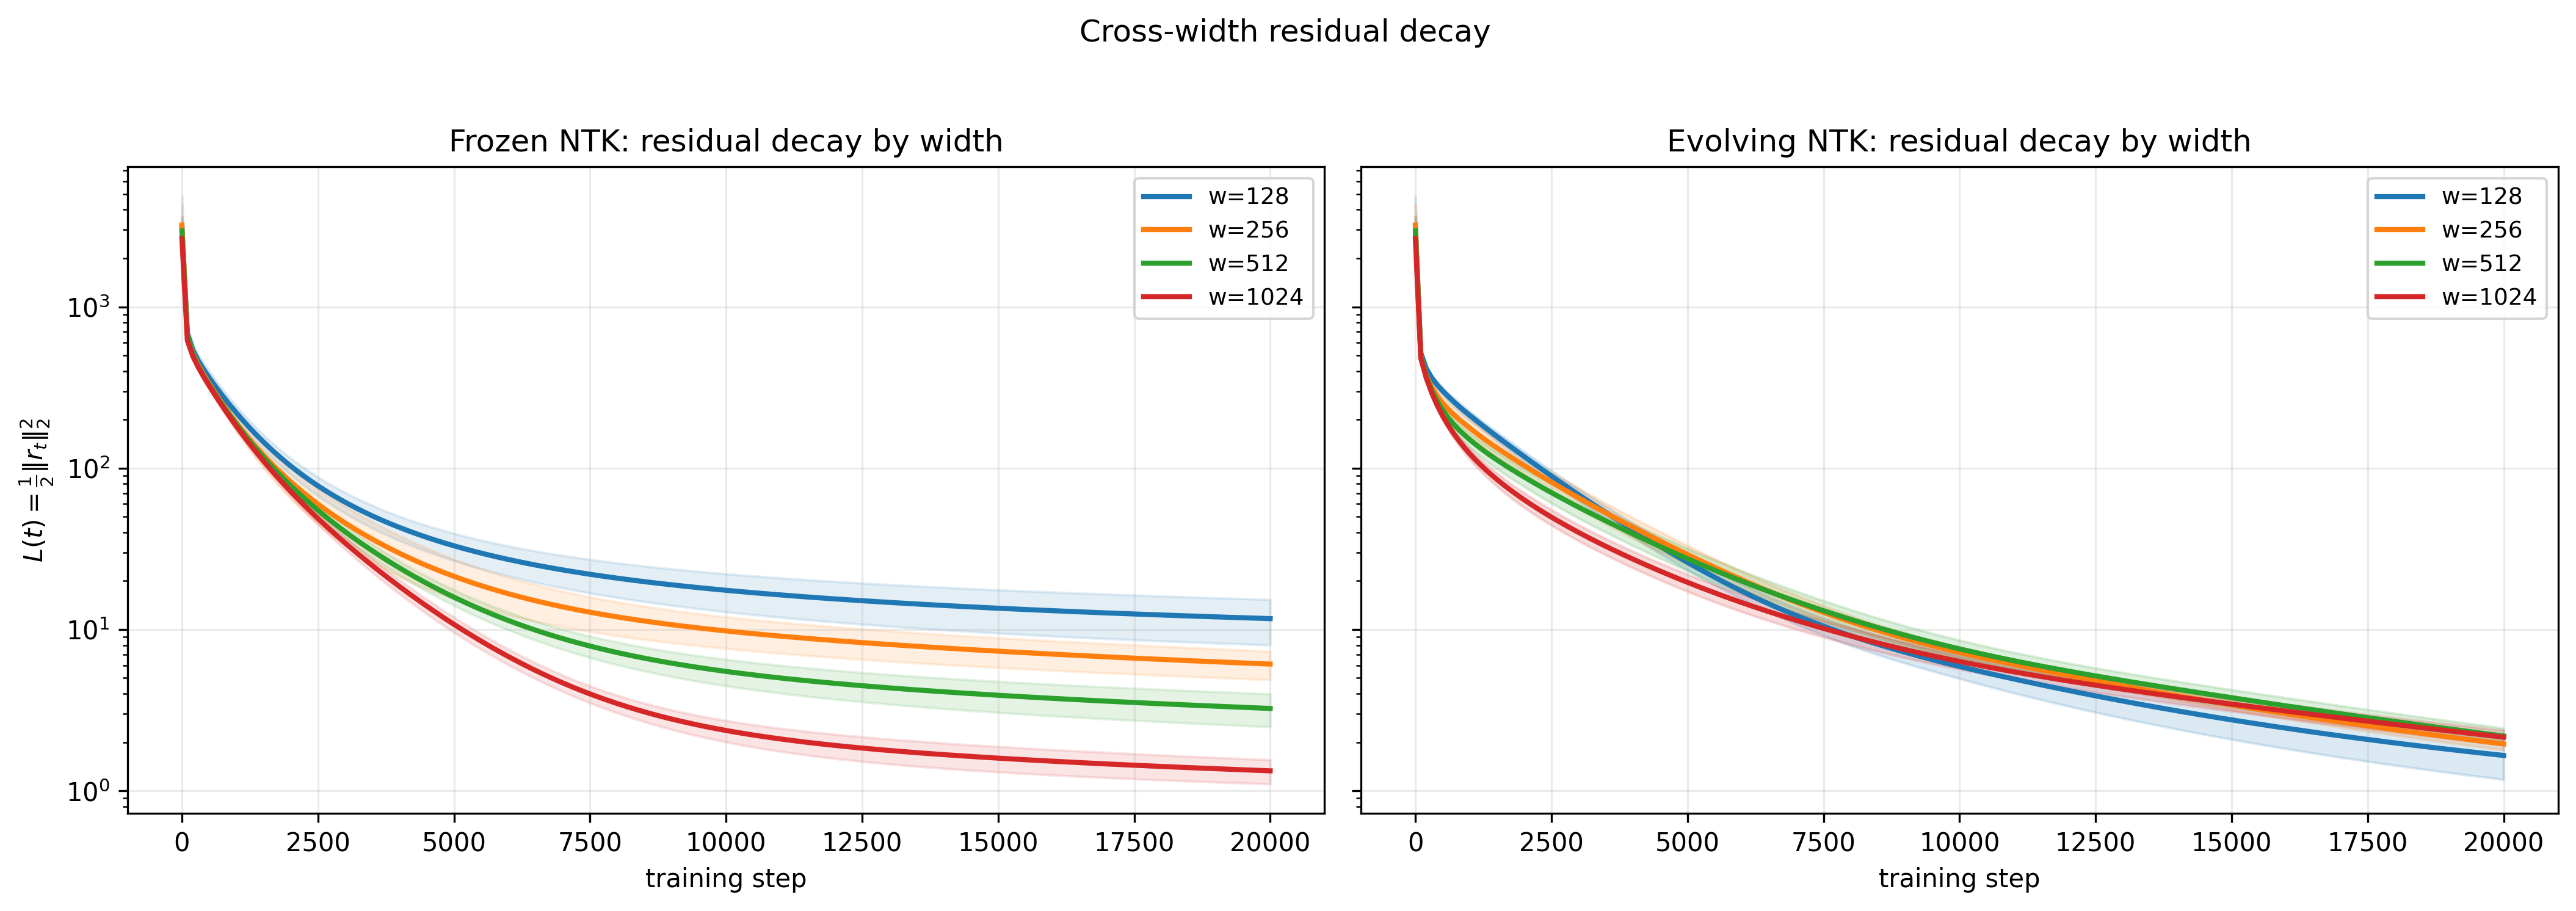
\includegraphics[width=0.95\textwidth]{images/finite_width_evolving_results/cross_width_residual_decay.png}
	\caption{Cross-width comparison of the least-squares objective
		\(L(t)=\frac{1}{2}\|r_t\|_2^2\) under frozen and evolving tangent-kernel
		dynamics. In the frozen regime, larger width gives consistently better
		residual decay. In the evolving regime, the curves are closer across widths.}
	\label{fig:evolving-cross-width-loss}
\end{figure}

\begin{figure}[!htbp]
	\centering
	\begin{subfigure}[t]{0.48\textwidth}
		\centering
		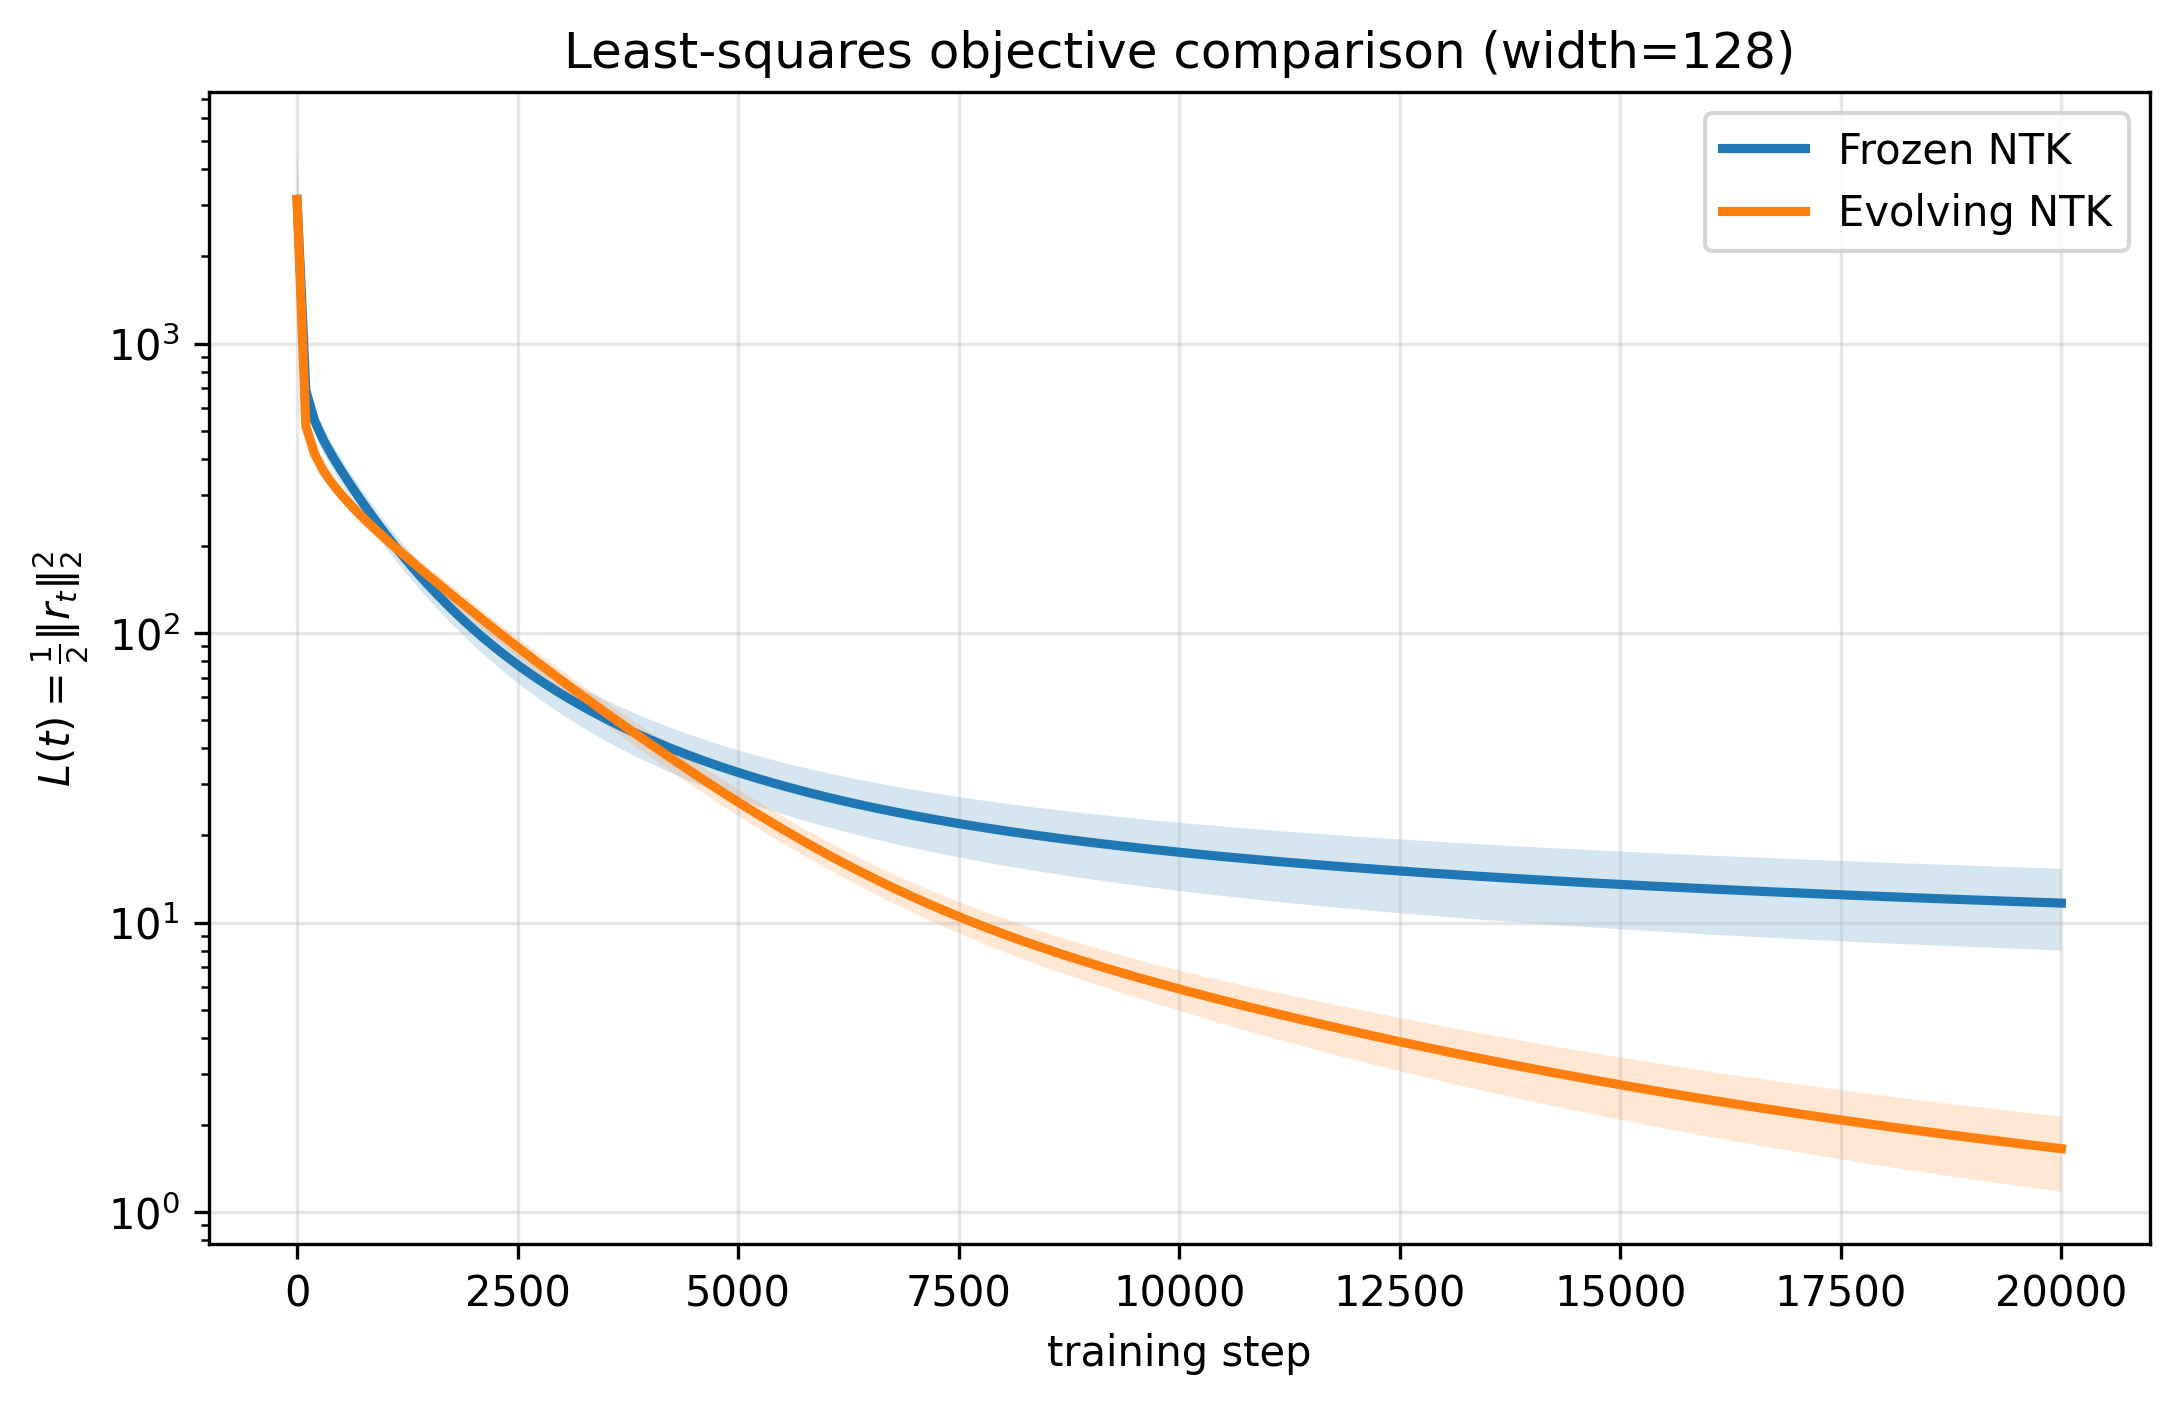
\includegraphics[width=\linewidth]{images/finite_width_evolving_results/train_ls_frozen_vs_evolving_w128.png}
		\caption{Width \(128\).}
	\end{subfigure}
	\hfill
	\begin{subfigure}[t]{0.48\textwidth}
		\centering
		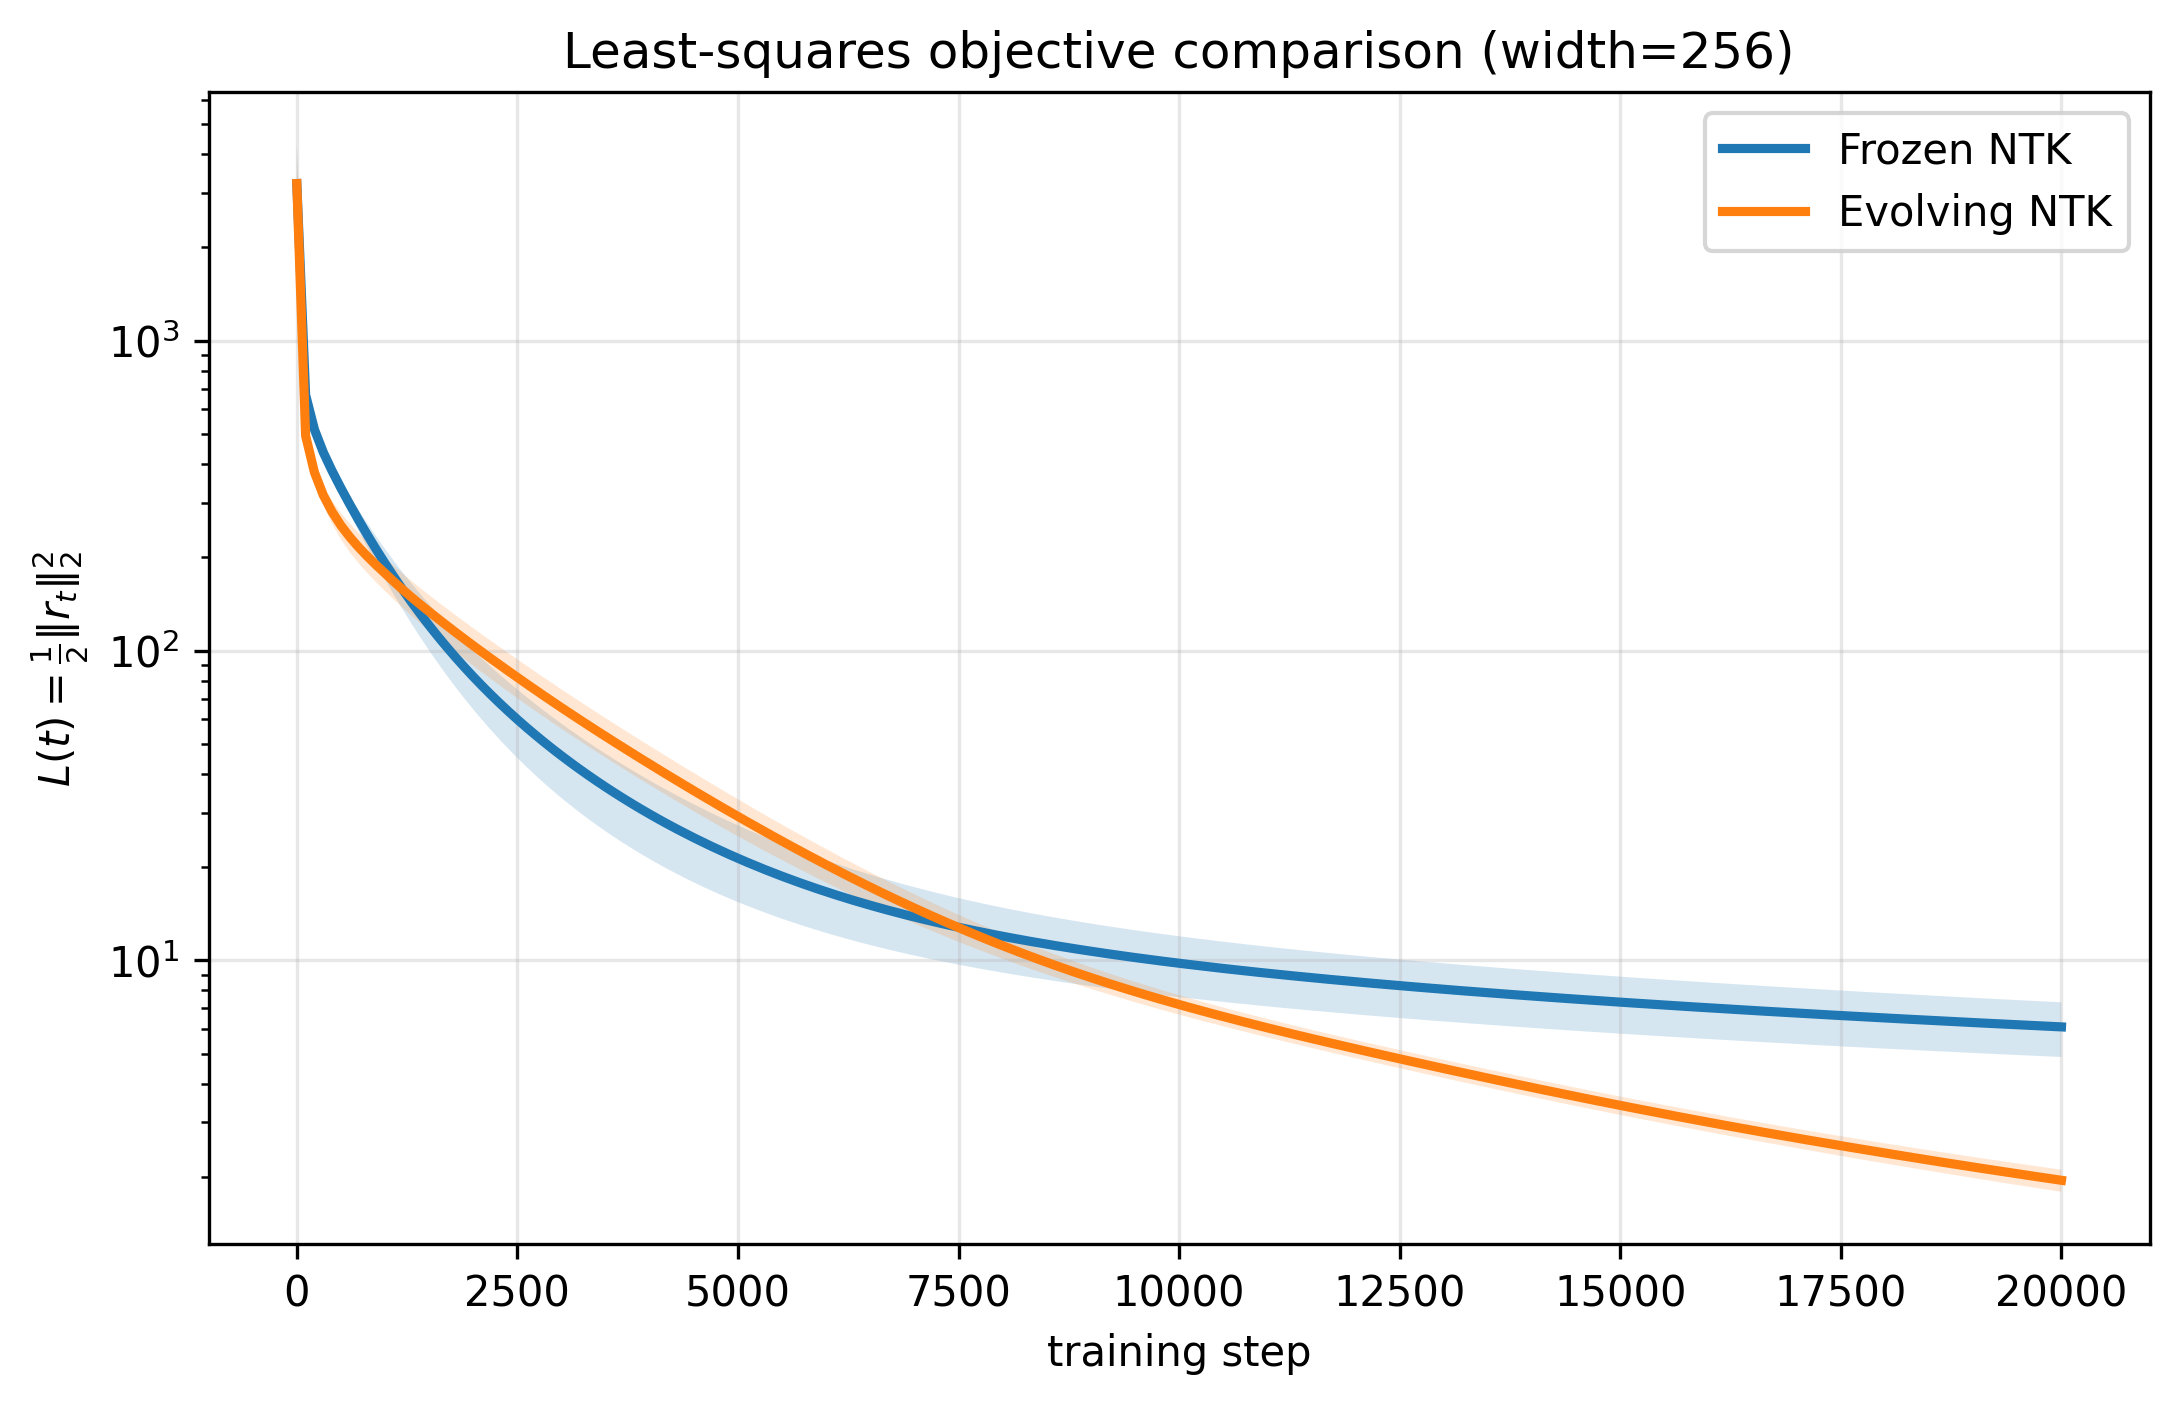
\includegraphics[width=\linewidth]{images/finite_width_evolving_results/train_ls_frozen_vs_evolving_w256.png}
		\caption{Width \(256\).}
	\end{subfigure}

	\vspace{0.6em}

	\begin{subfigure}[t]{0.48\textwidth}
		\centering
		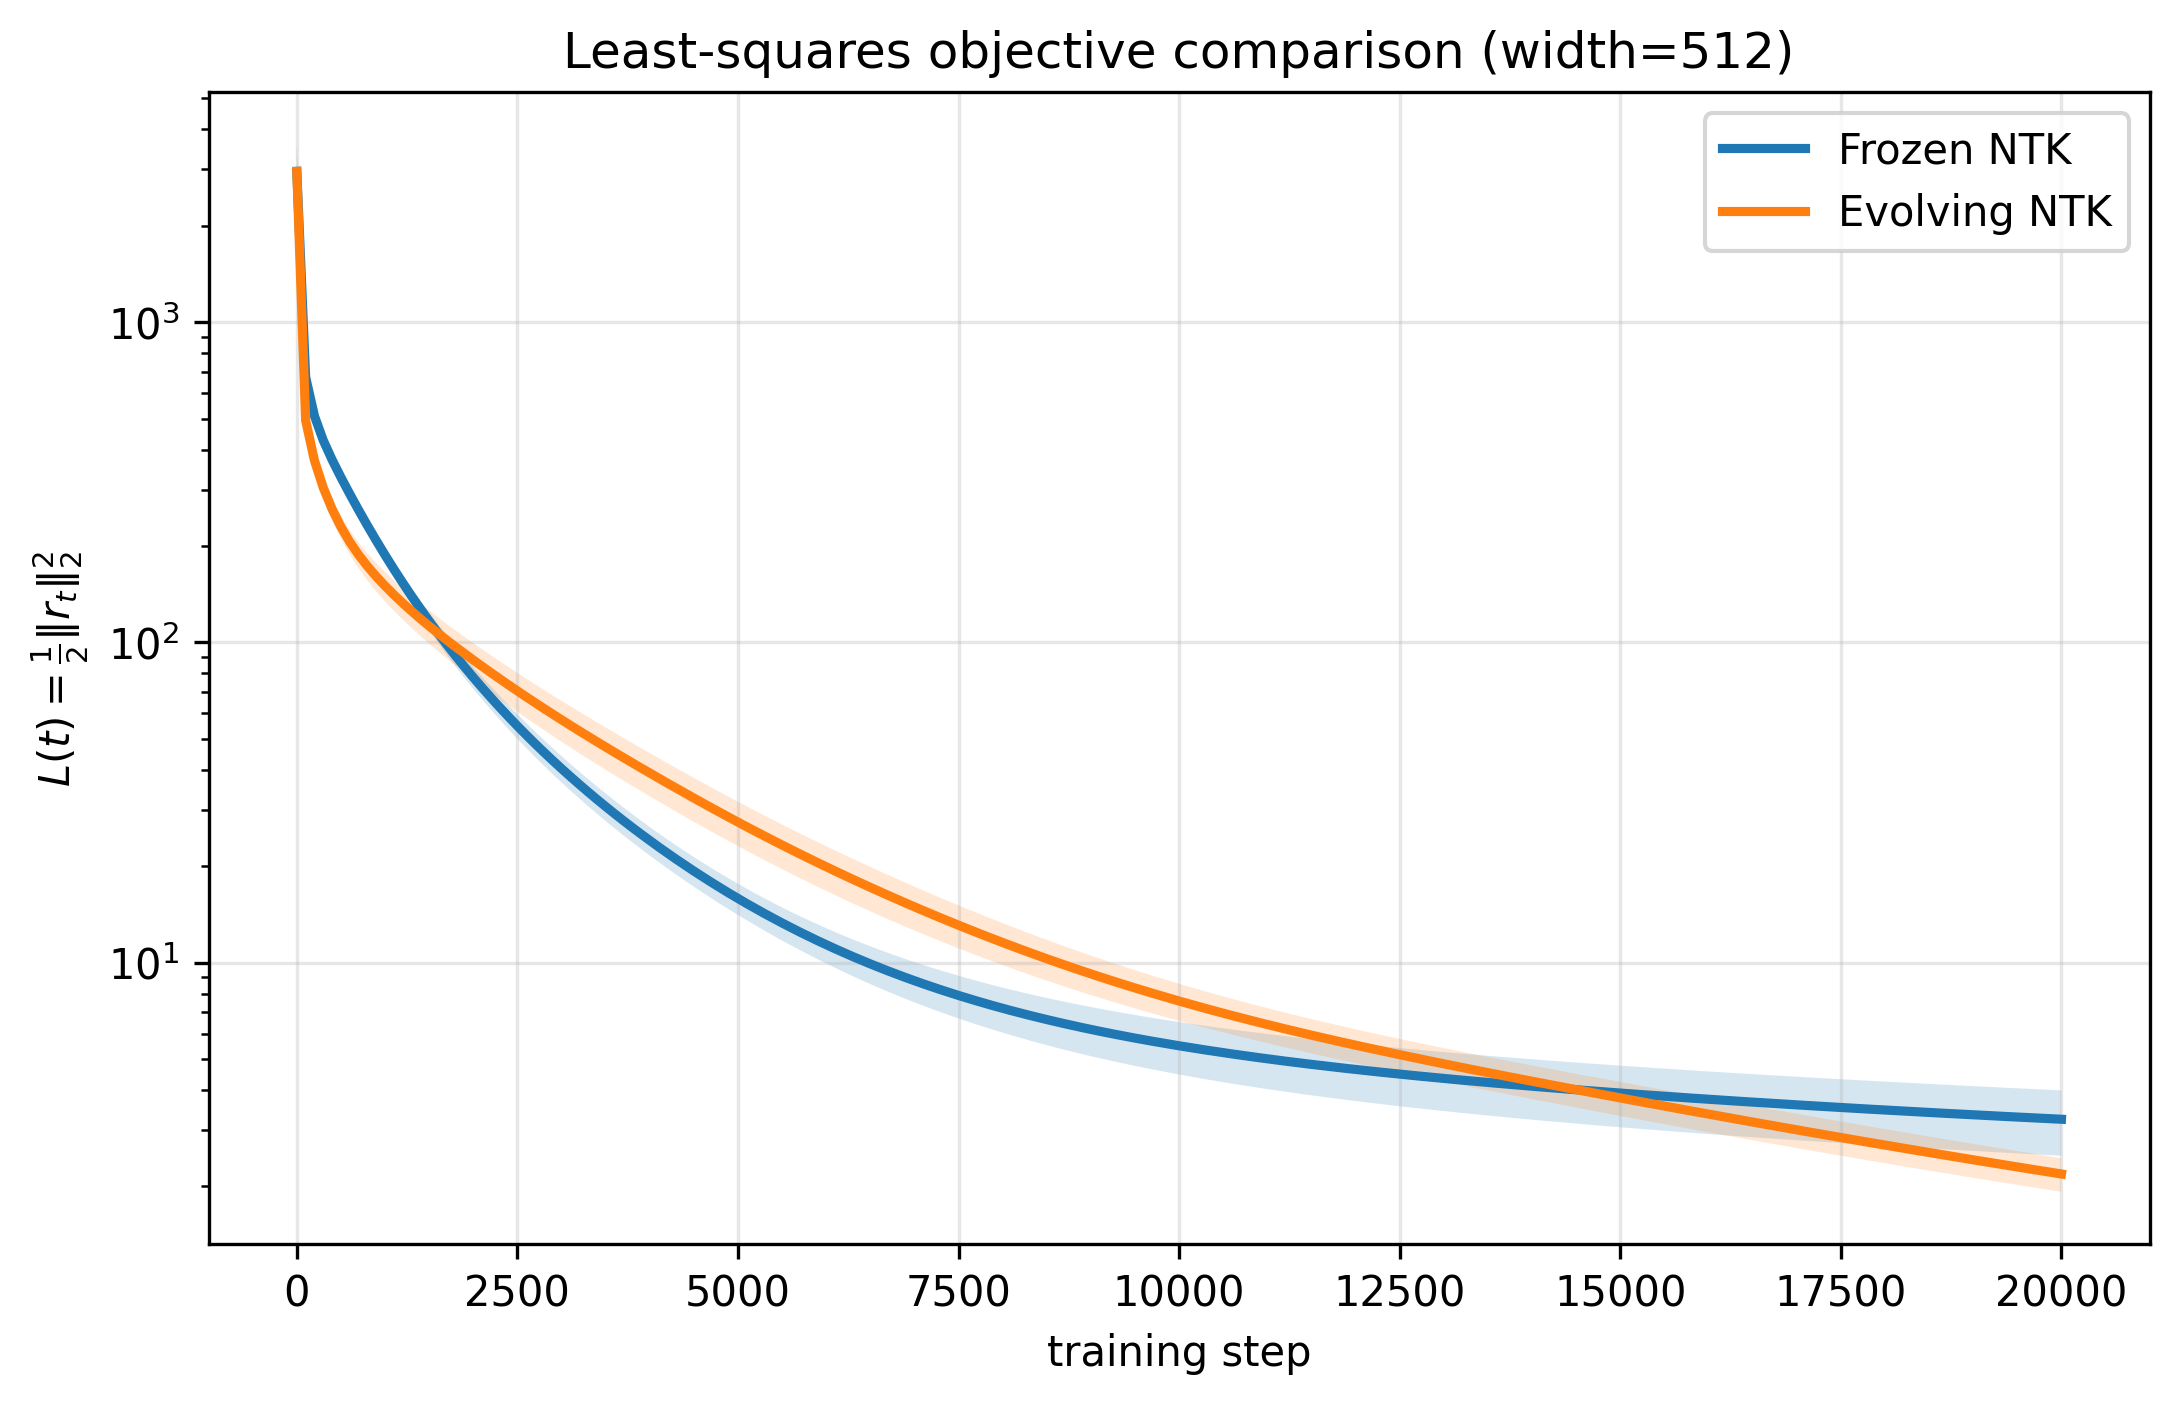
\includegraphics[width=\linewidth]{images/finite_width_evolving_results/train_ls_frozen_vs_evolving_w512.png}
		\caption{Width \(512\).}
	\end{subfigure}
	\hfill
	\begin{subfigure}[t]{0.48\textwidth}
		\centering
		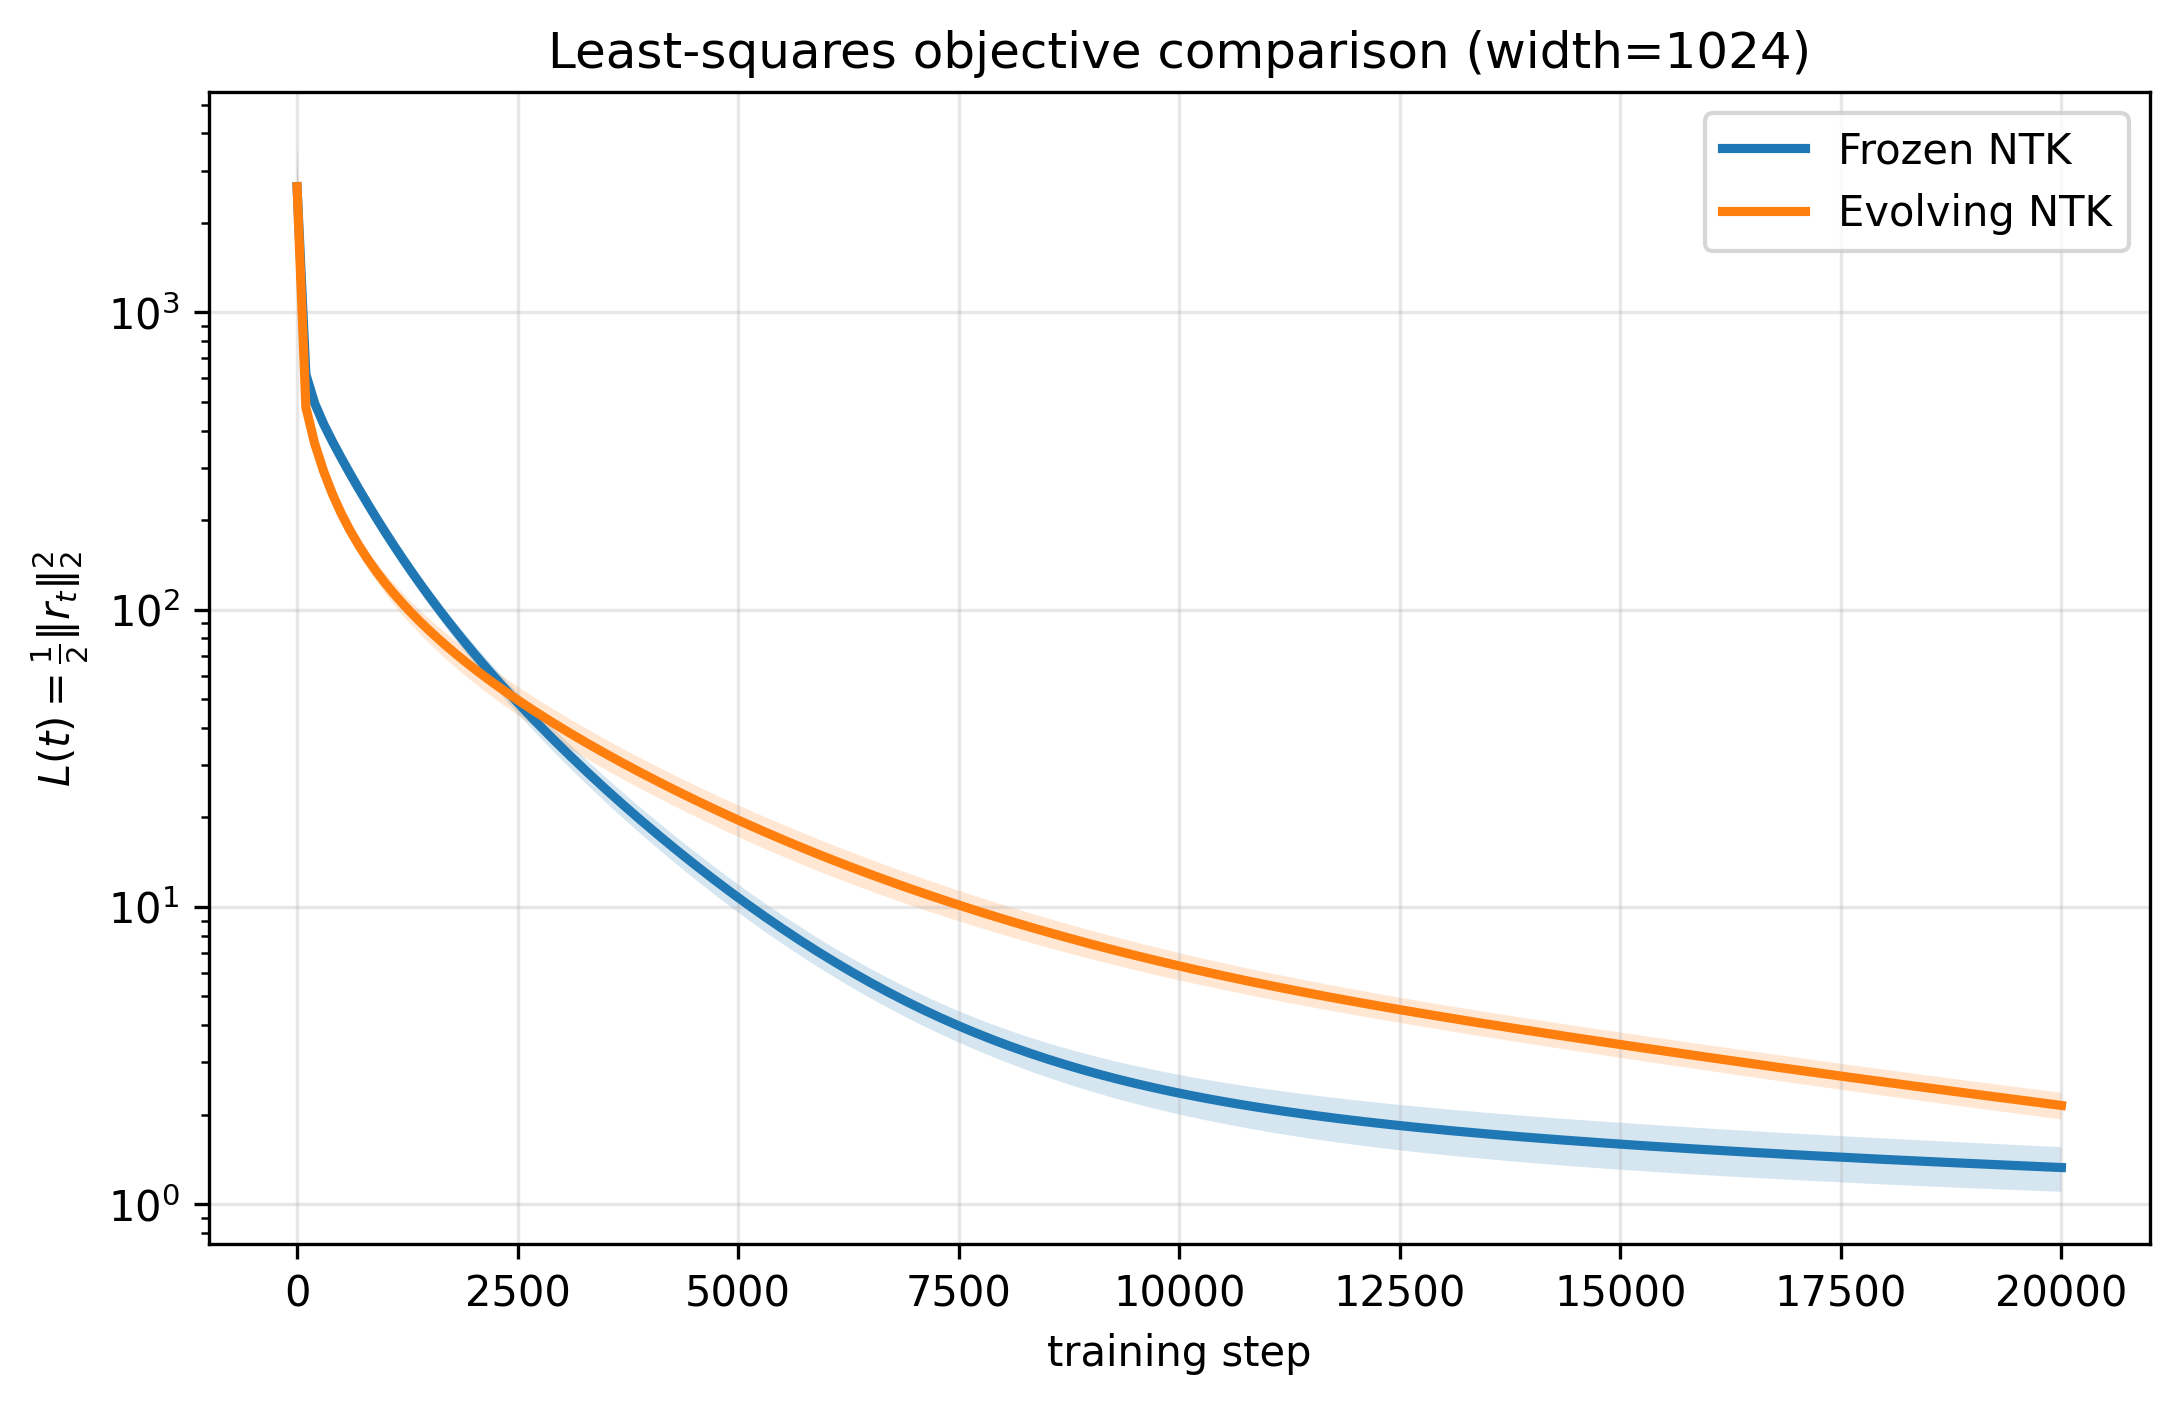
\includegraphics[width=\linewidth]{images/finite_width_evolving_results/train_ls_frozen_vs_evolving_w1024.png}
		\caption{Width \(1024\).}
	\end{subfigure}
	\caption{Least-squares objective comparison between frozen and evolving
		finite-width tangent-kernel dynamics across widths. The evolving kernel gives
		a clear improvement at widths \(128\) and \(256\), still improves the final
		objective at width \(512\), and loses its advantage by width \(1024\), where
		the frozen kernel reaches the lower final loss.}
	\label{fig:evolving-loss-by-width}
\end{figure}

In the frozen regime, the objective decreases more quickly as the width
increases. In the evolving regime, the curves are more tightly clustered across
widths. At widths \(128\) and \(256\), the evolving kernel reaches a lower final
objective than the frozen baseline. At width \(512\), the difference is smaller.
At width \(1024\), the frozen kernel reaches the lower final objective.

This raises the main question for the rest of the section: what changes in the
evolving tangent kernel allow it to help at small width, but not at large
width?

\subsection{Mode-wise decay, Fourier geometry, and spectral strength}
\label{subsec:results-evolving-joint}

To understand the loss comparison above, we examine three quantities together.
The mode-wise residual decay plots show how individual Fourier components are
learned over time. The subspace cosine similarity plots measure how closely the
eigenspaces of the evolving tangent-kernel remain aligned with the Fourier subspaces.
The spectral-strength plots measure the average eigenvalue inside each Fourier
block. This quantity can be read as the average strength with which the current
kernel acts on that Fourier subspace: larger spectral strength means that
residual components in that block are pushed down more strongly by the kernel
dynamics.

If the evolving kernel helps because it preserves Fourier geometry better, then
one would expect improved alignment in the subspaces over time. If instead it
helps by redistributing operator strength, then one should expect improved
decay of the low-frequency residual modes together with increased low-frequency
spectral strength, even if the Fourier alignment worsens.

\begin{figure}[!htbp]
	\centering

	\begin{subfigure}[t]{\textwidth}
		\centering
		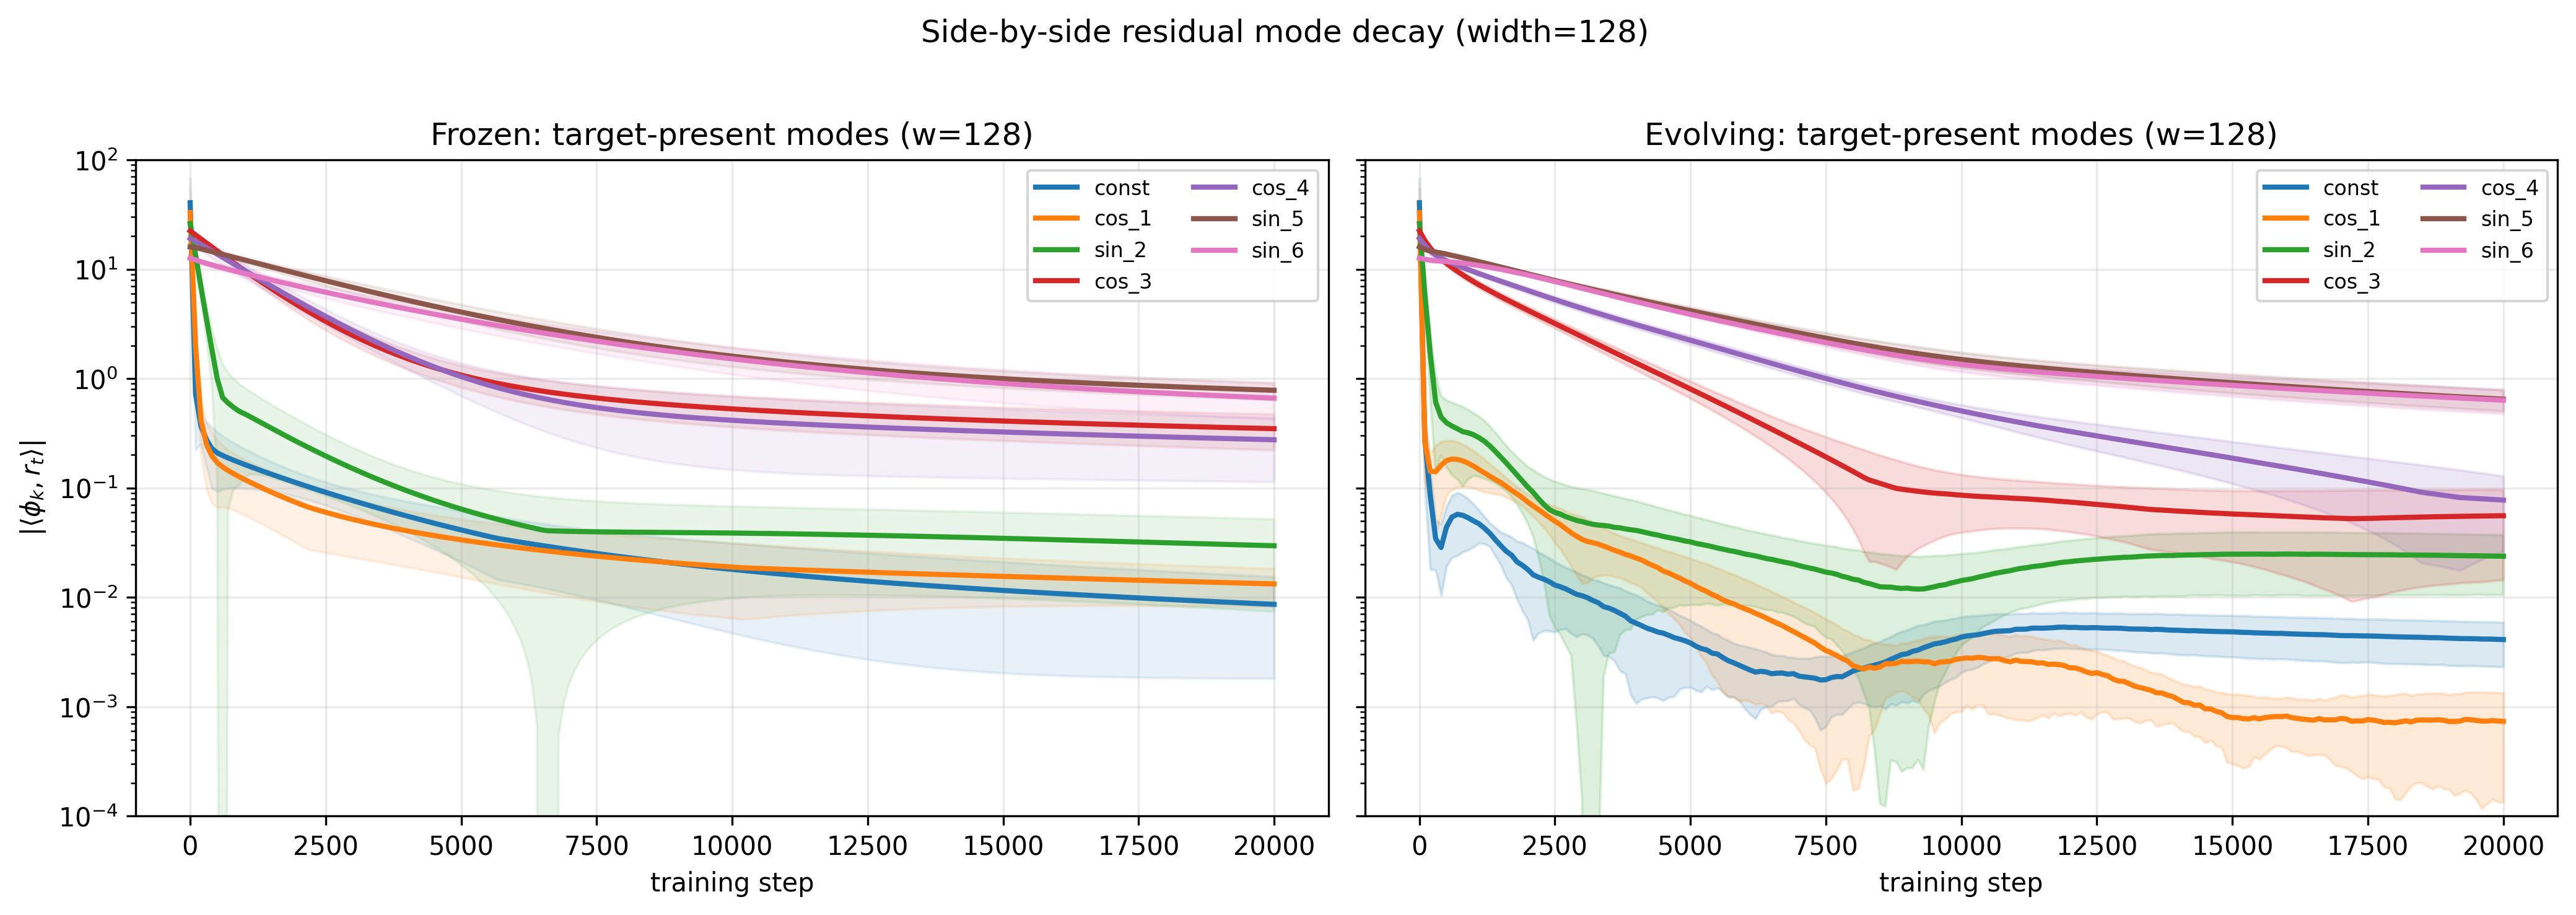
\includegraphics[width=\linewidth]{images/finite_width_evolving_results/side_by_side_residual_decay_w128.png}
		\caption{Mode-wise residual decay.}
	\end{subfigure}

	\vspace{0.8em}

	\begin{subfigure}[t]{\textwidth}
		\centering
		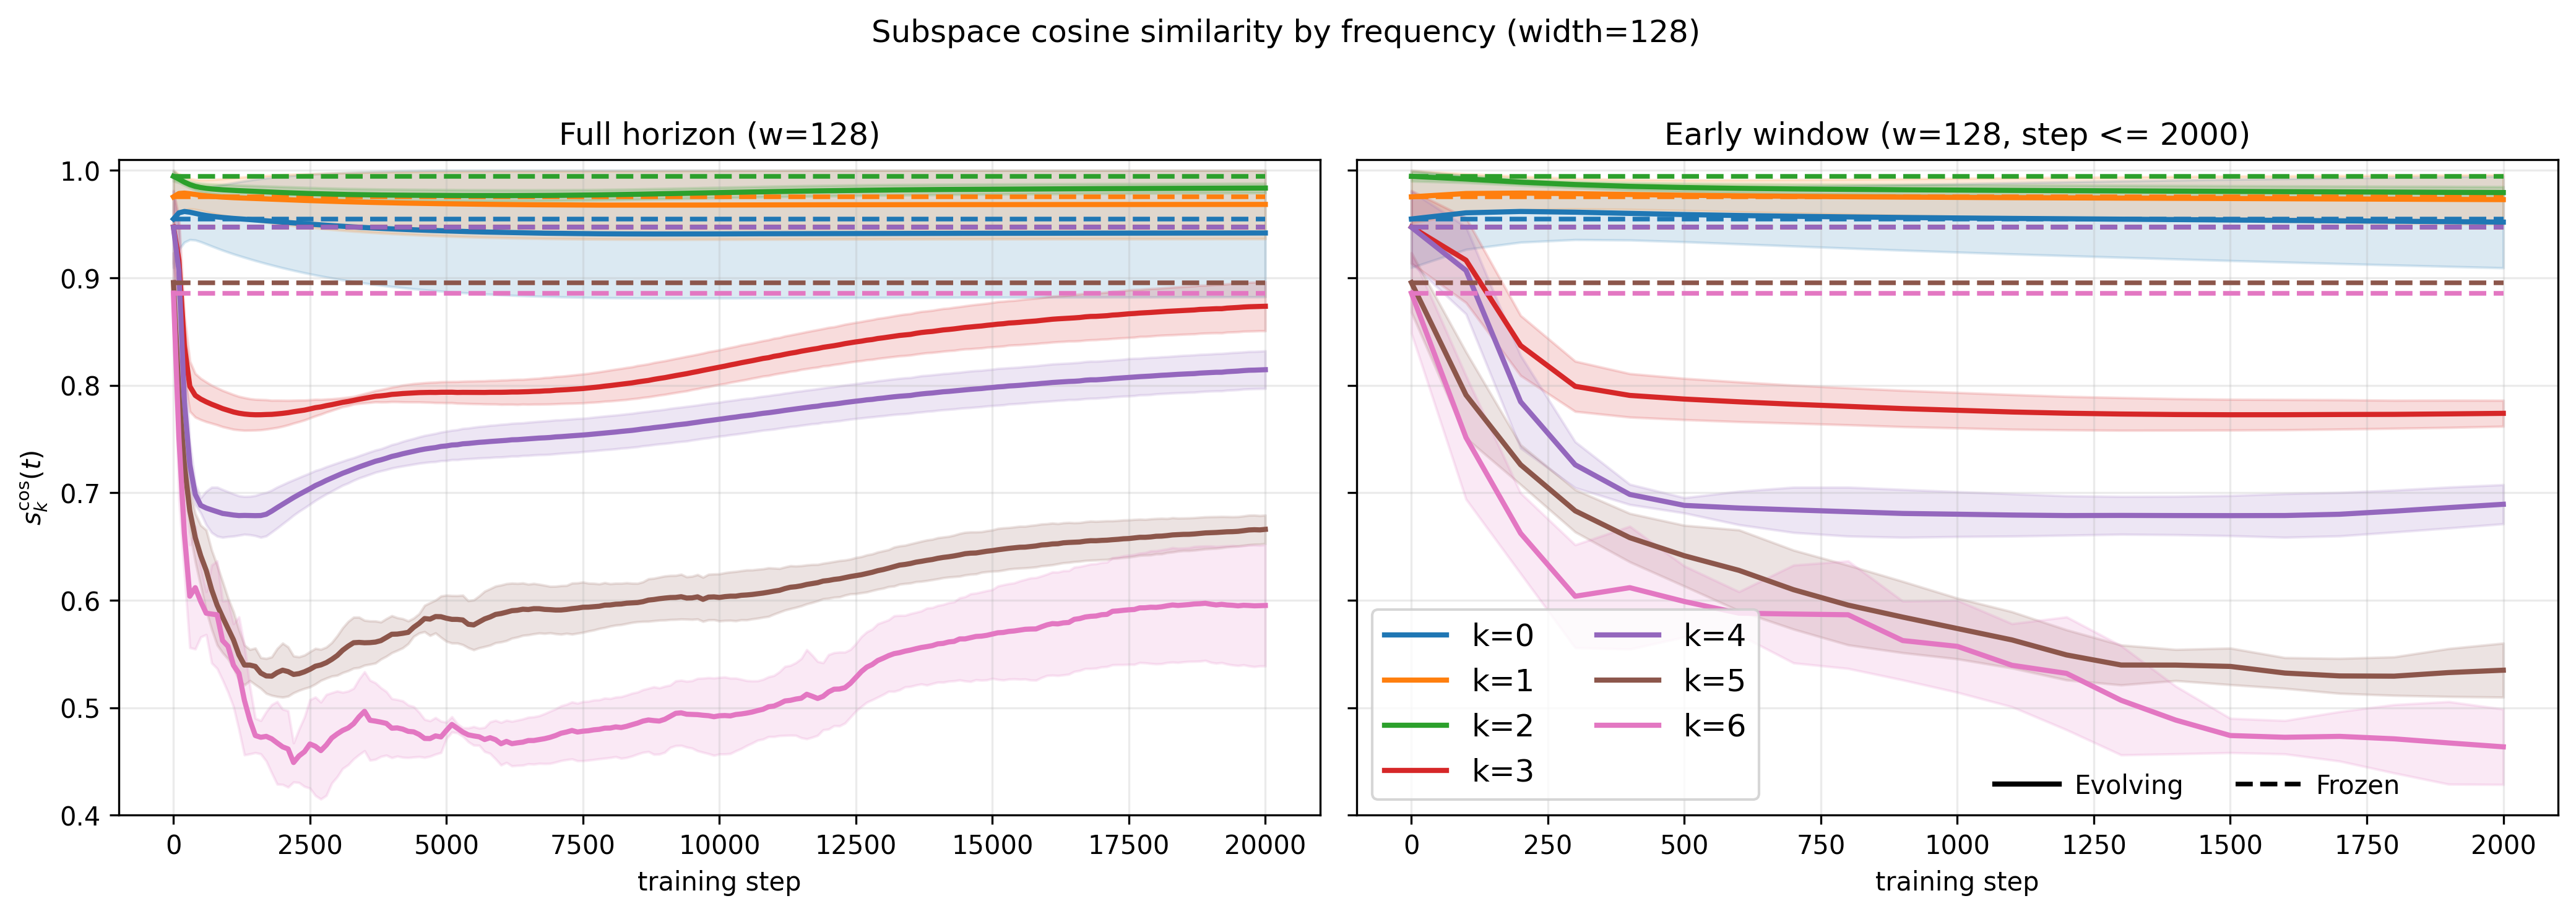
\includegraphics[width=\linewidth]{images/finite_width_evolving_results/rms_cos_alignment_by_freq_w128.png}
		\caption{Subspace cosine similarity.}
	\end{subfigure}

	\vspace{0.8em}

	\begin{subfigure}[t]{\textwidth}
		\centering
		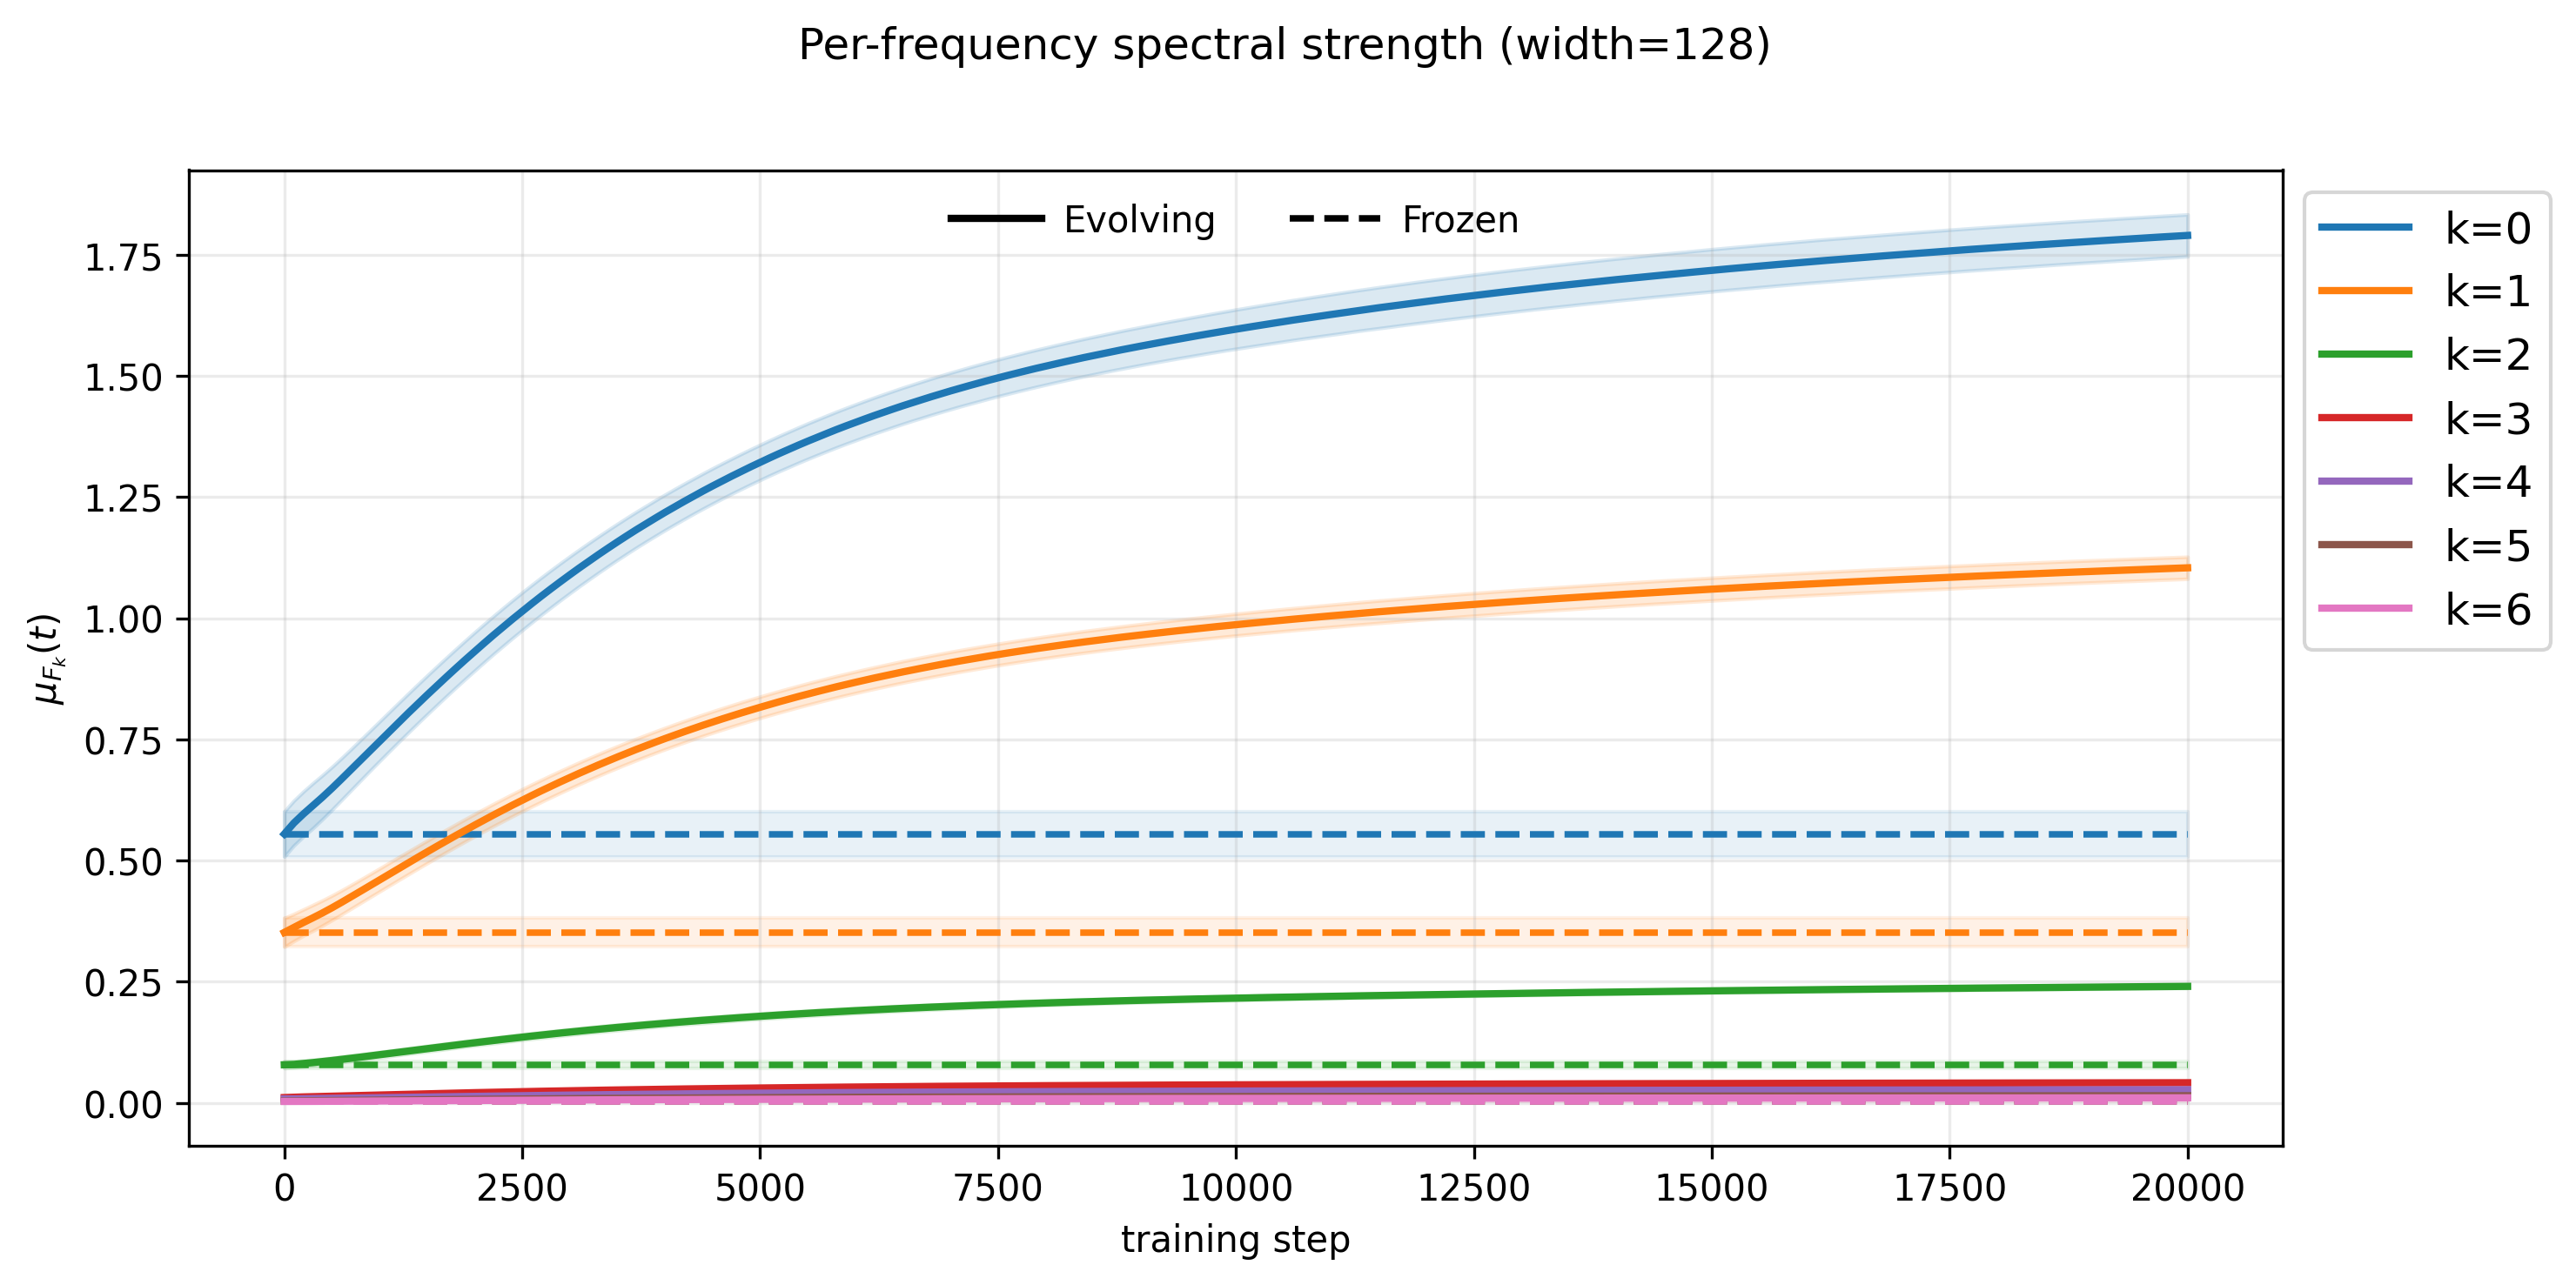
\includegraphics[width=\linewidth]{images/finite_width_evolving_results/spectral_strength_by_freq_w128.png}
		\caption{Per-frequency spectral strength.}
	\end{subfigure}

	\caption{Joint diagnostics for the evolving finite-width tangent kernel at
		width \(128\). The top panel compares frozen and evolving residual decay for
		the target-present modes. The middle panel measures Fourier-subspace
		alignment. The bottom panel measures the average tangent-kernel strength
		inside each Fourier block.}
	\label{fig:evolving-joint-w128}
\end{figure}

\begin{figure}[!htbp]
	\centering

	\begin{subfigure}[t]{\textwidth}
		\centering
		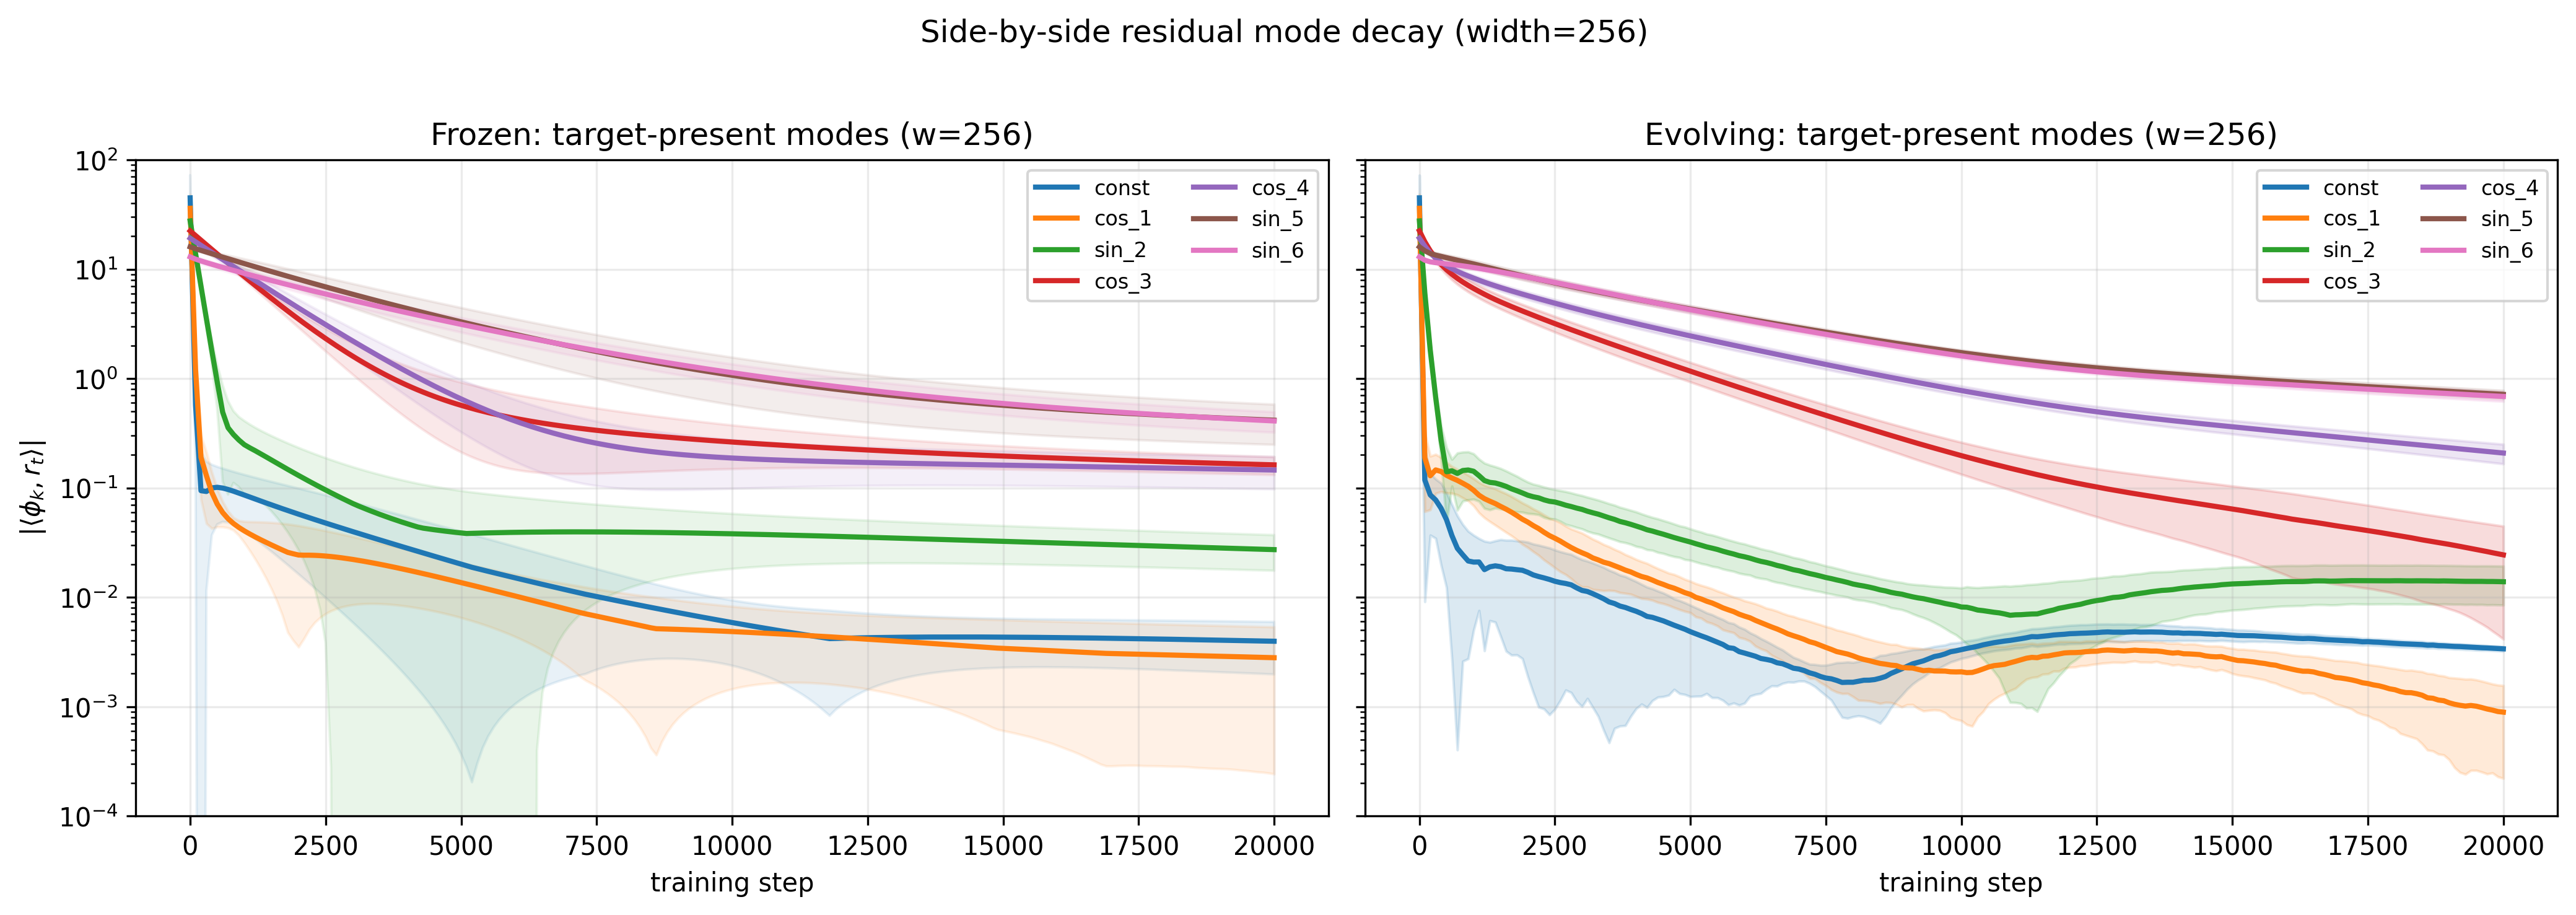
\includegraphics[width=\linewidth]{images/finite_width_evolving_results/side_by_side_residual_decay_w256.png}
		\caption{Mode-wise residual decay.}
	\end{subfigure}

	\vspace{0.8em}

	\begin{subfigure}[t]{\textwidth}
		\centering
		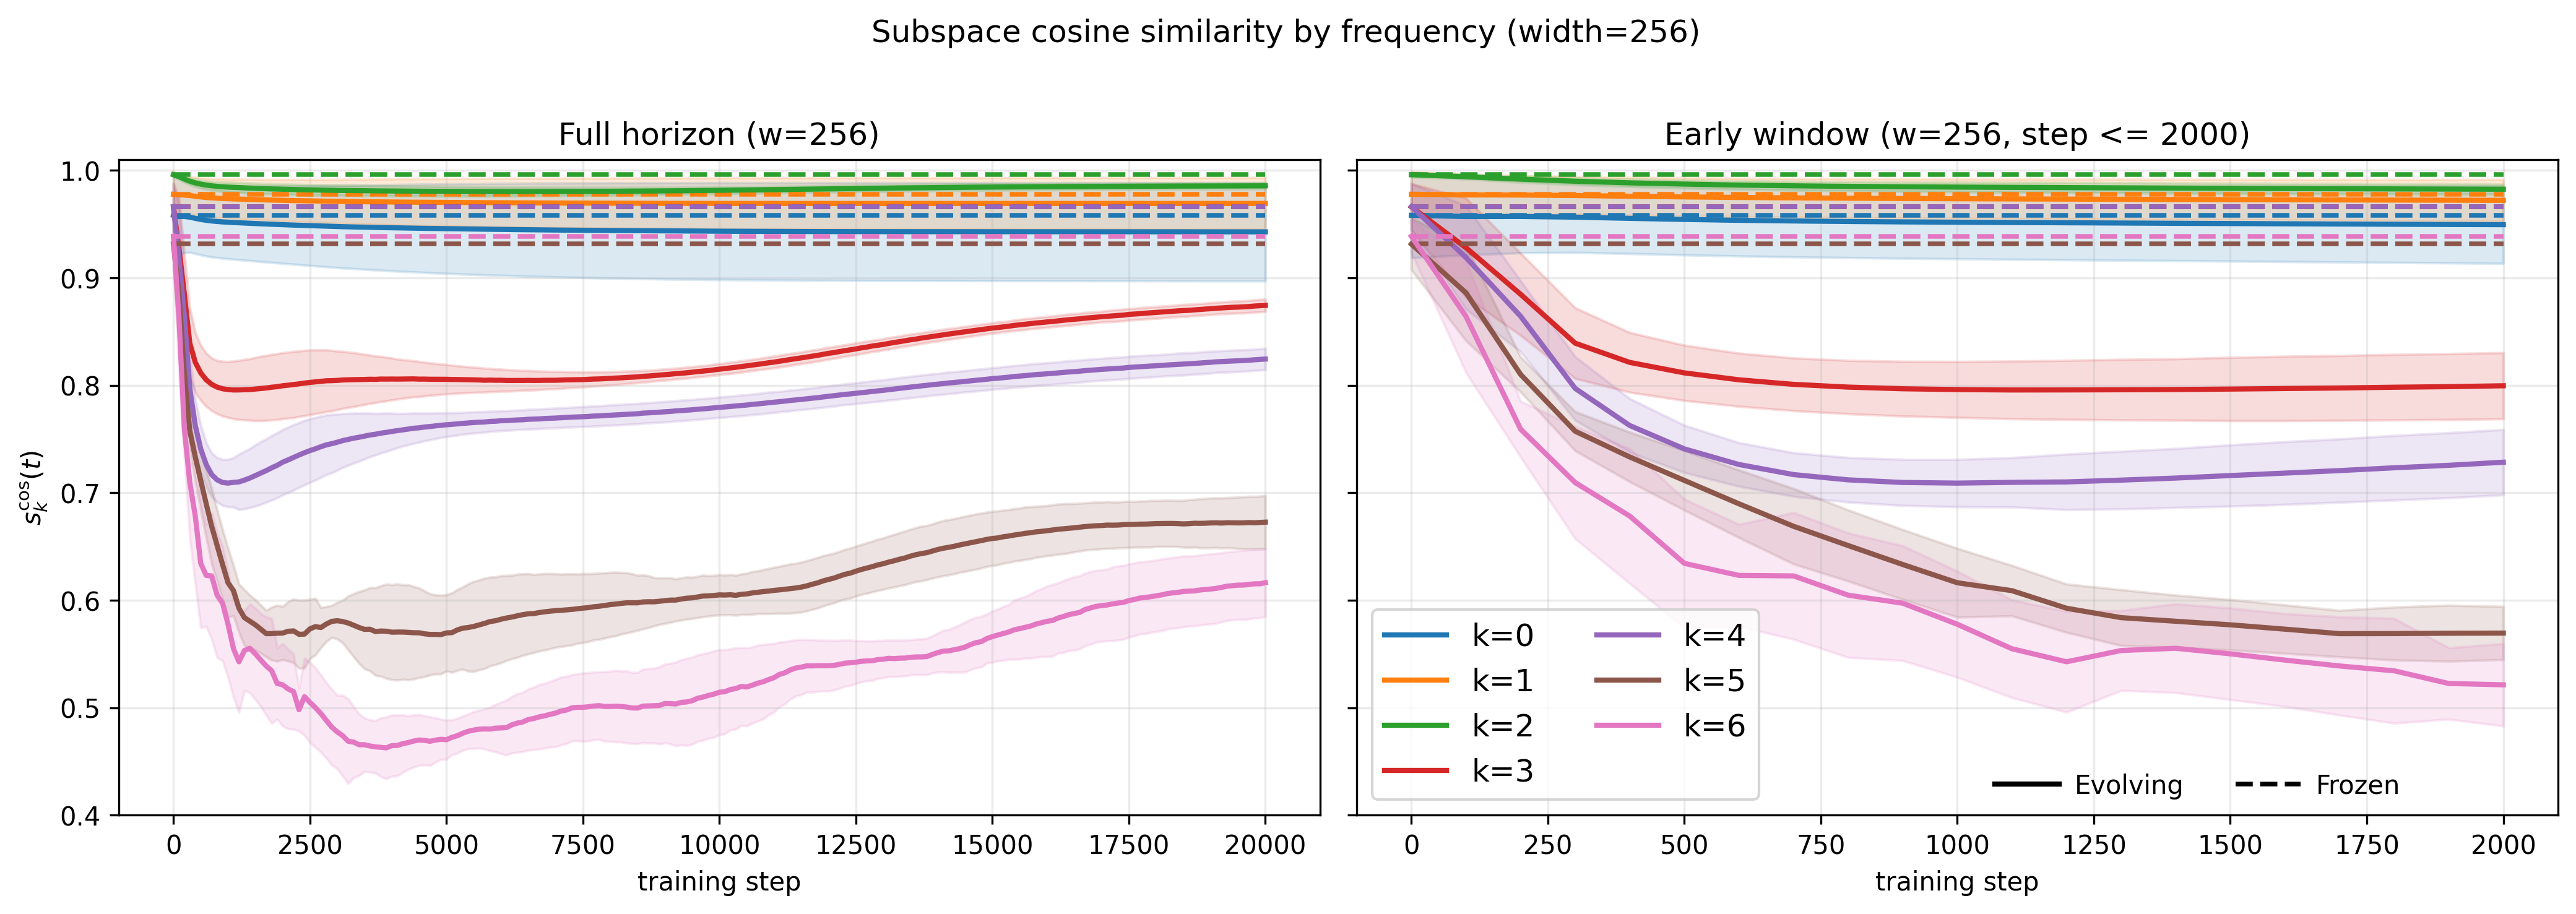
\includegraphics[width=\linewidth]{images/finite_width_evolving_results/rms_cos_alignment_by_freq_w256.png}
		\caption{Subspace cosine similarity.}
	\end{subfigure}

	\vspace{0.8em}

	\begin{subfigure}[t]{\textwidth}
		\centering
		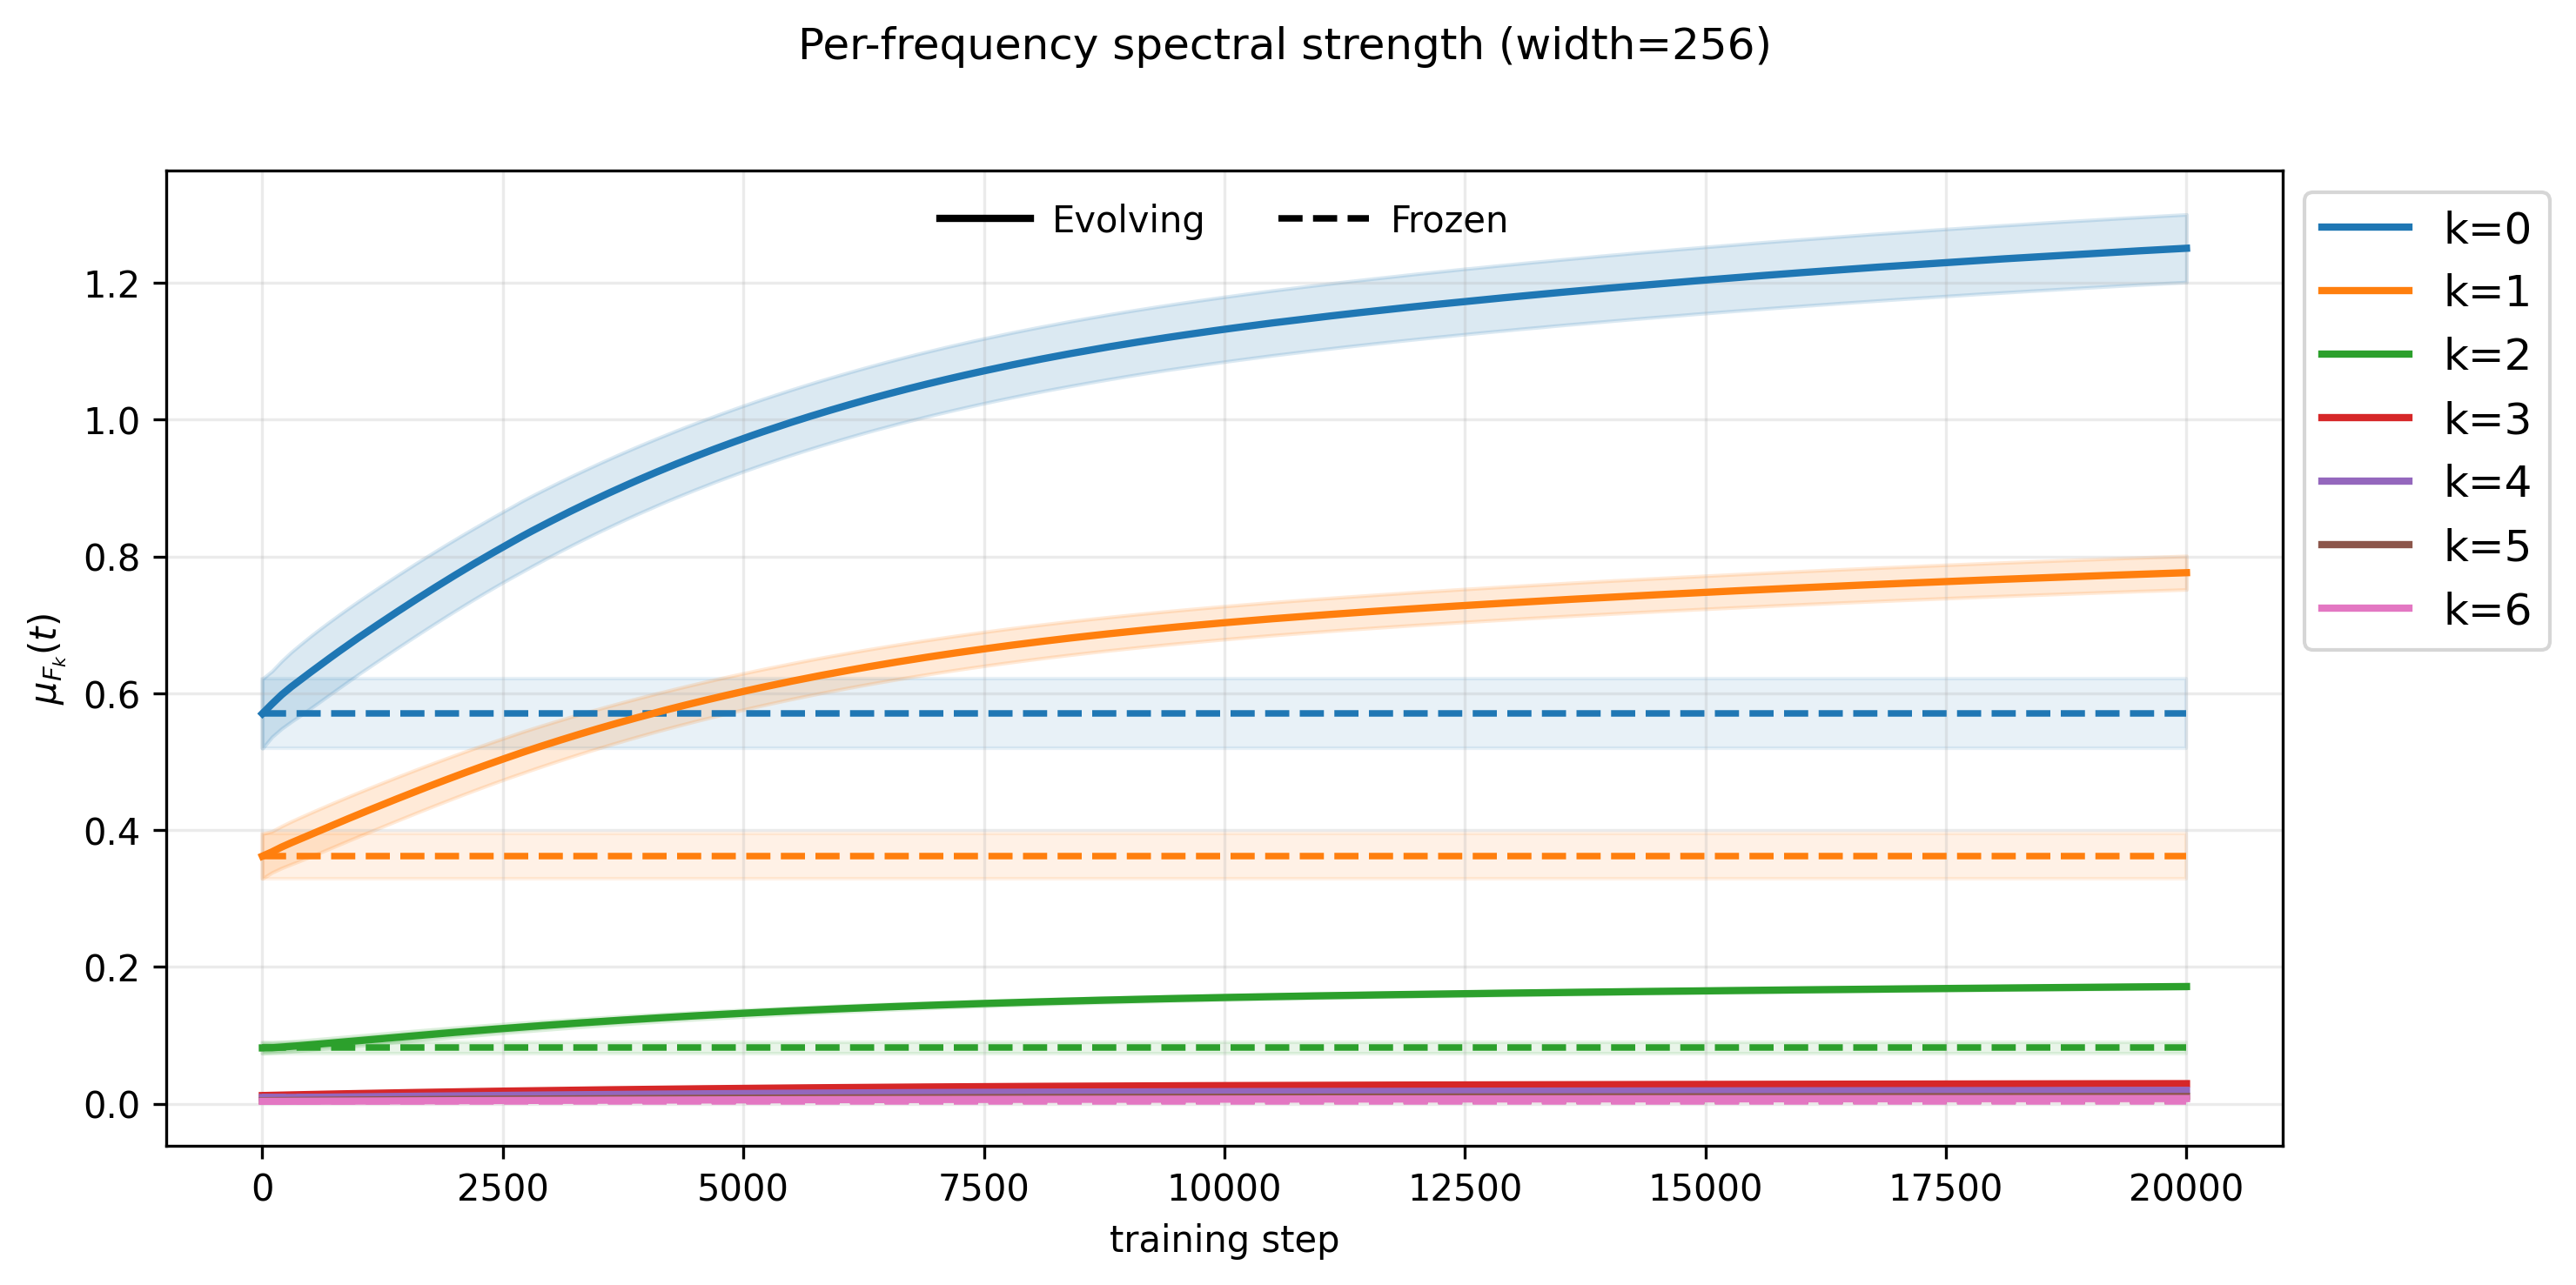
\includegraphics[width=\linewidth]{images/finite_width_evolving_results/spectral_strength_by_freq_w256.png}
		\caption{Per-frequency spectral strength.}
	\end{subfigure}

	\caption{Joint diagnostics for the evolving finite-width tangent kernel at
		width \(256\).}
	\label{fig:evolving-joint-w256}
\end{figure}

\begin{figure}[!htbp]
	\centering

	\begin{subfigure}[t]{\textwidth}
		\centering
		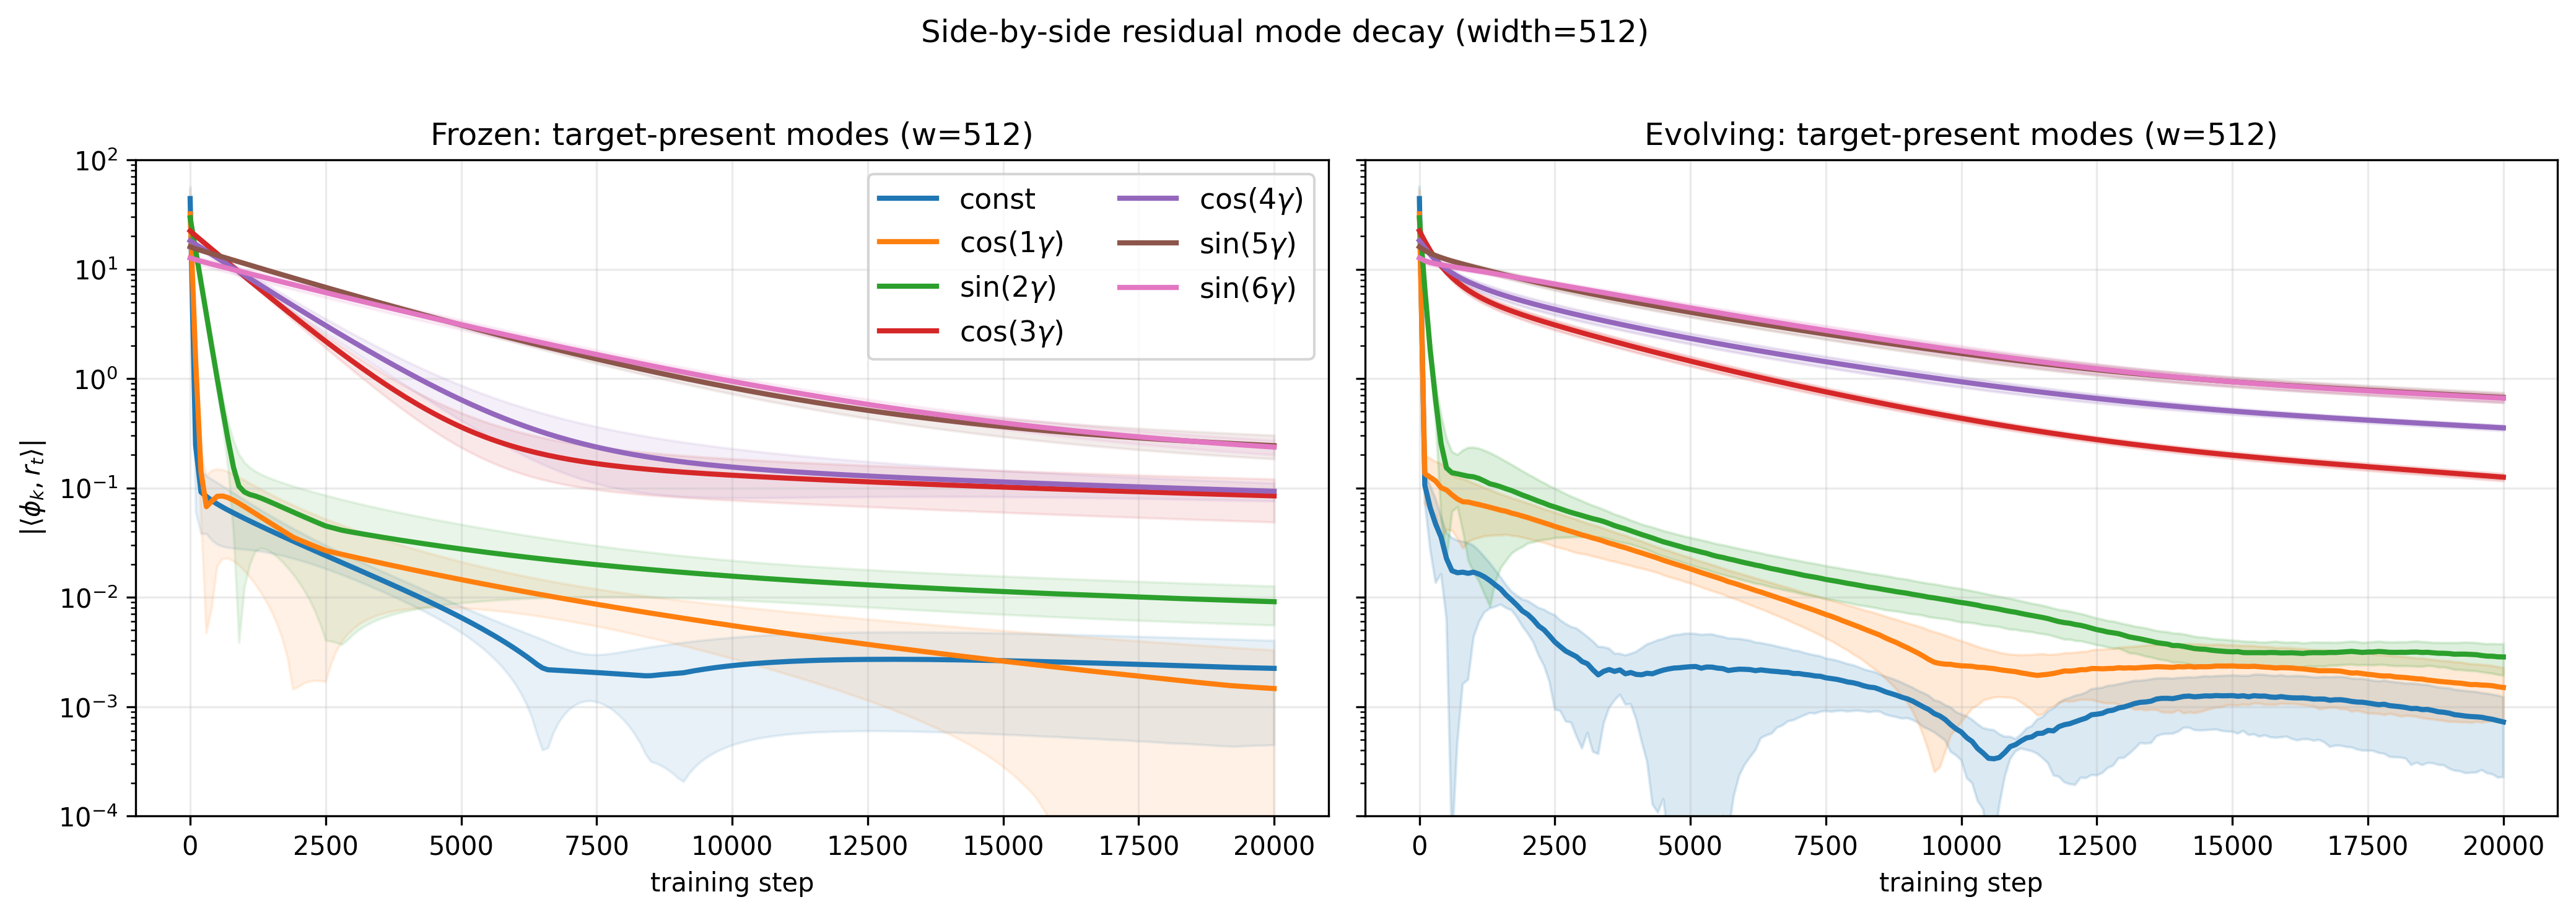
\includegraphics[width=\linewidth]{images/finite_width_evolving_results/side_by_side_residual_decay_w512.png}
		\caption{Mode-wise residual decay.}
	\end{subfigure}

	\vspace{0.8em}

	\begin{subfigure}[t]{\textwidth}
		\centering
		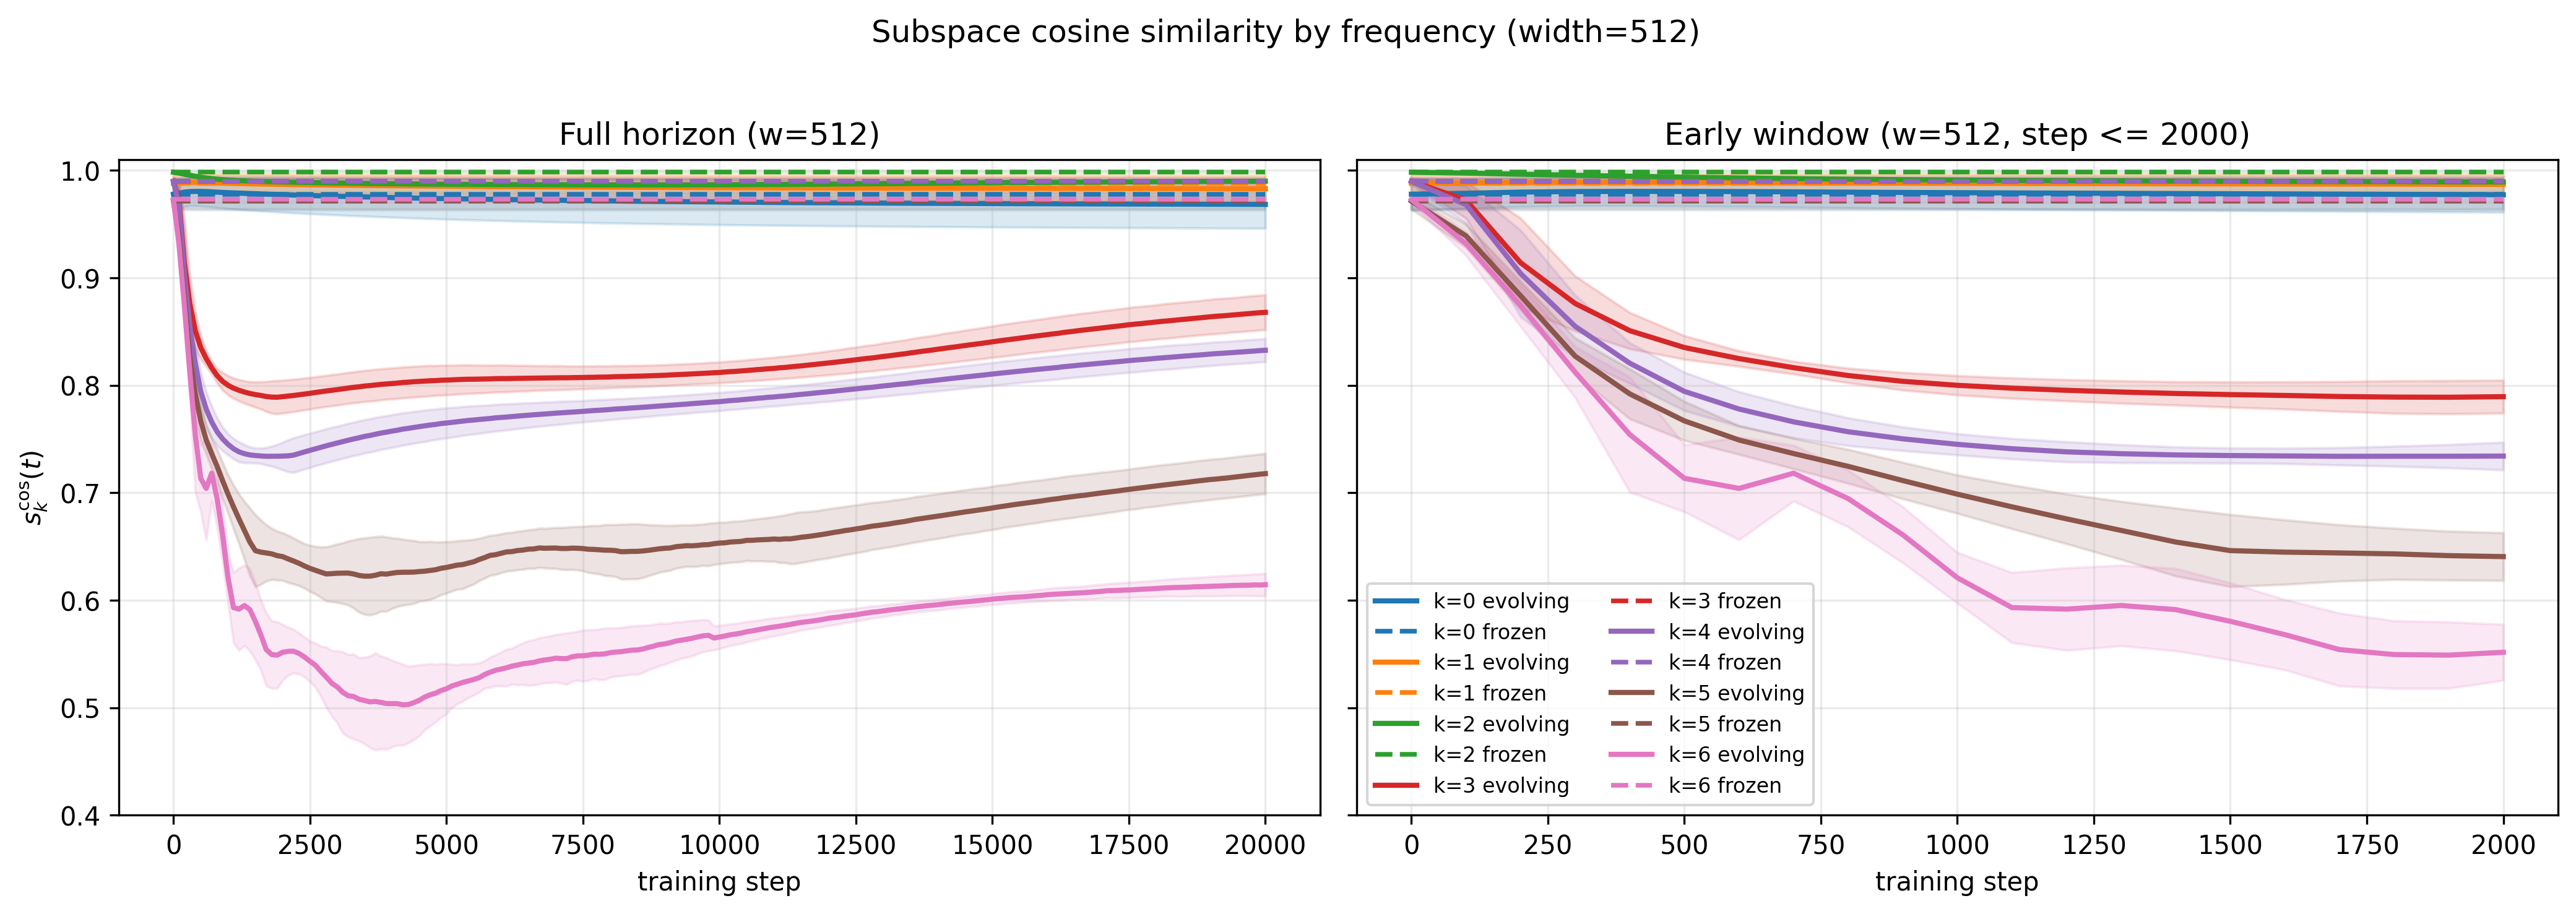
\includegraphics[width=\linewidth]{images/finite_width_evolving_results/rms_cos_alignment_by_freq_w512.png}
		\caption{Subspace cosine similarity.}
	\end{subfigure}

	\vspace{0.8em}

	\begin{subfigure}[t]{\textwidth}
		\centering
		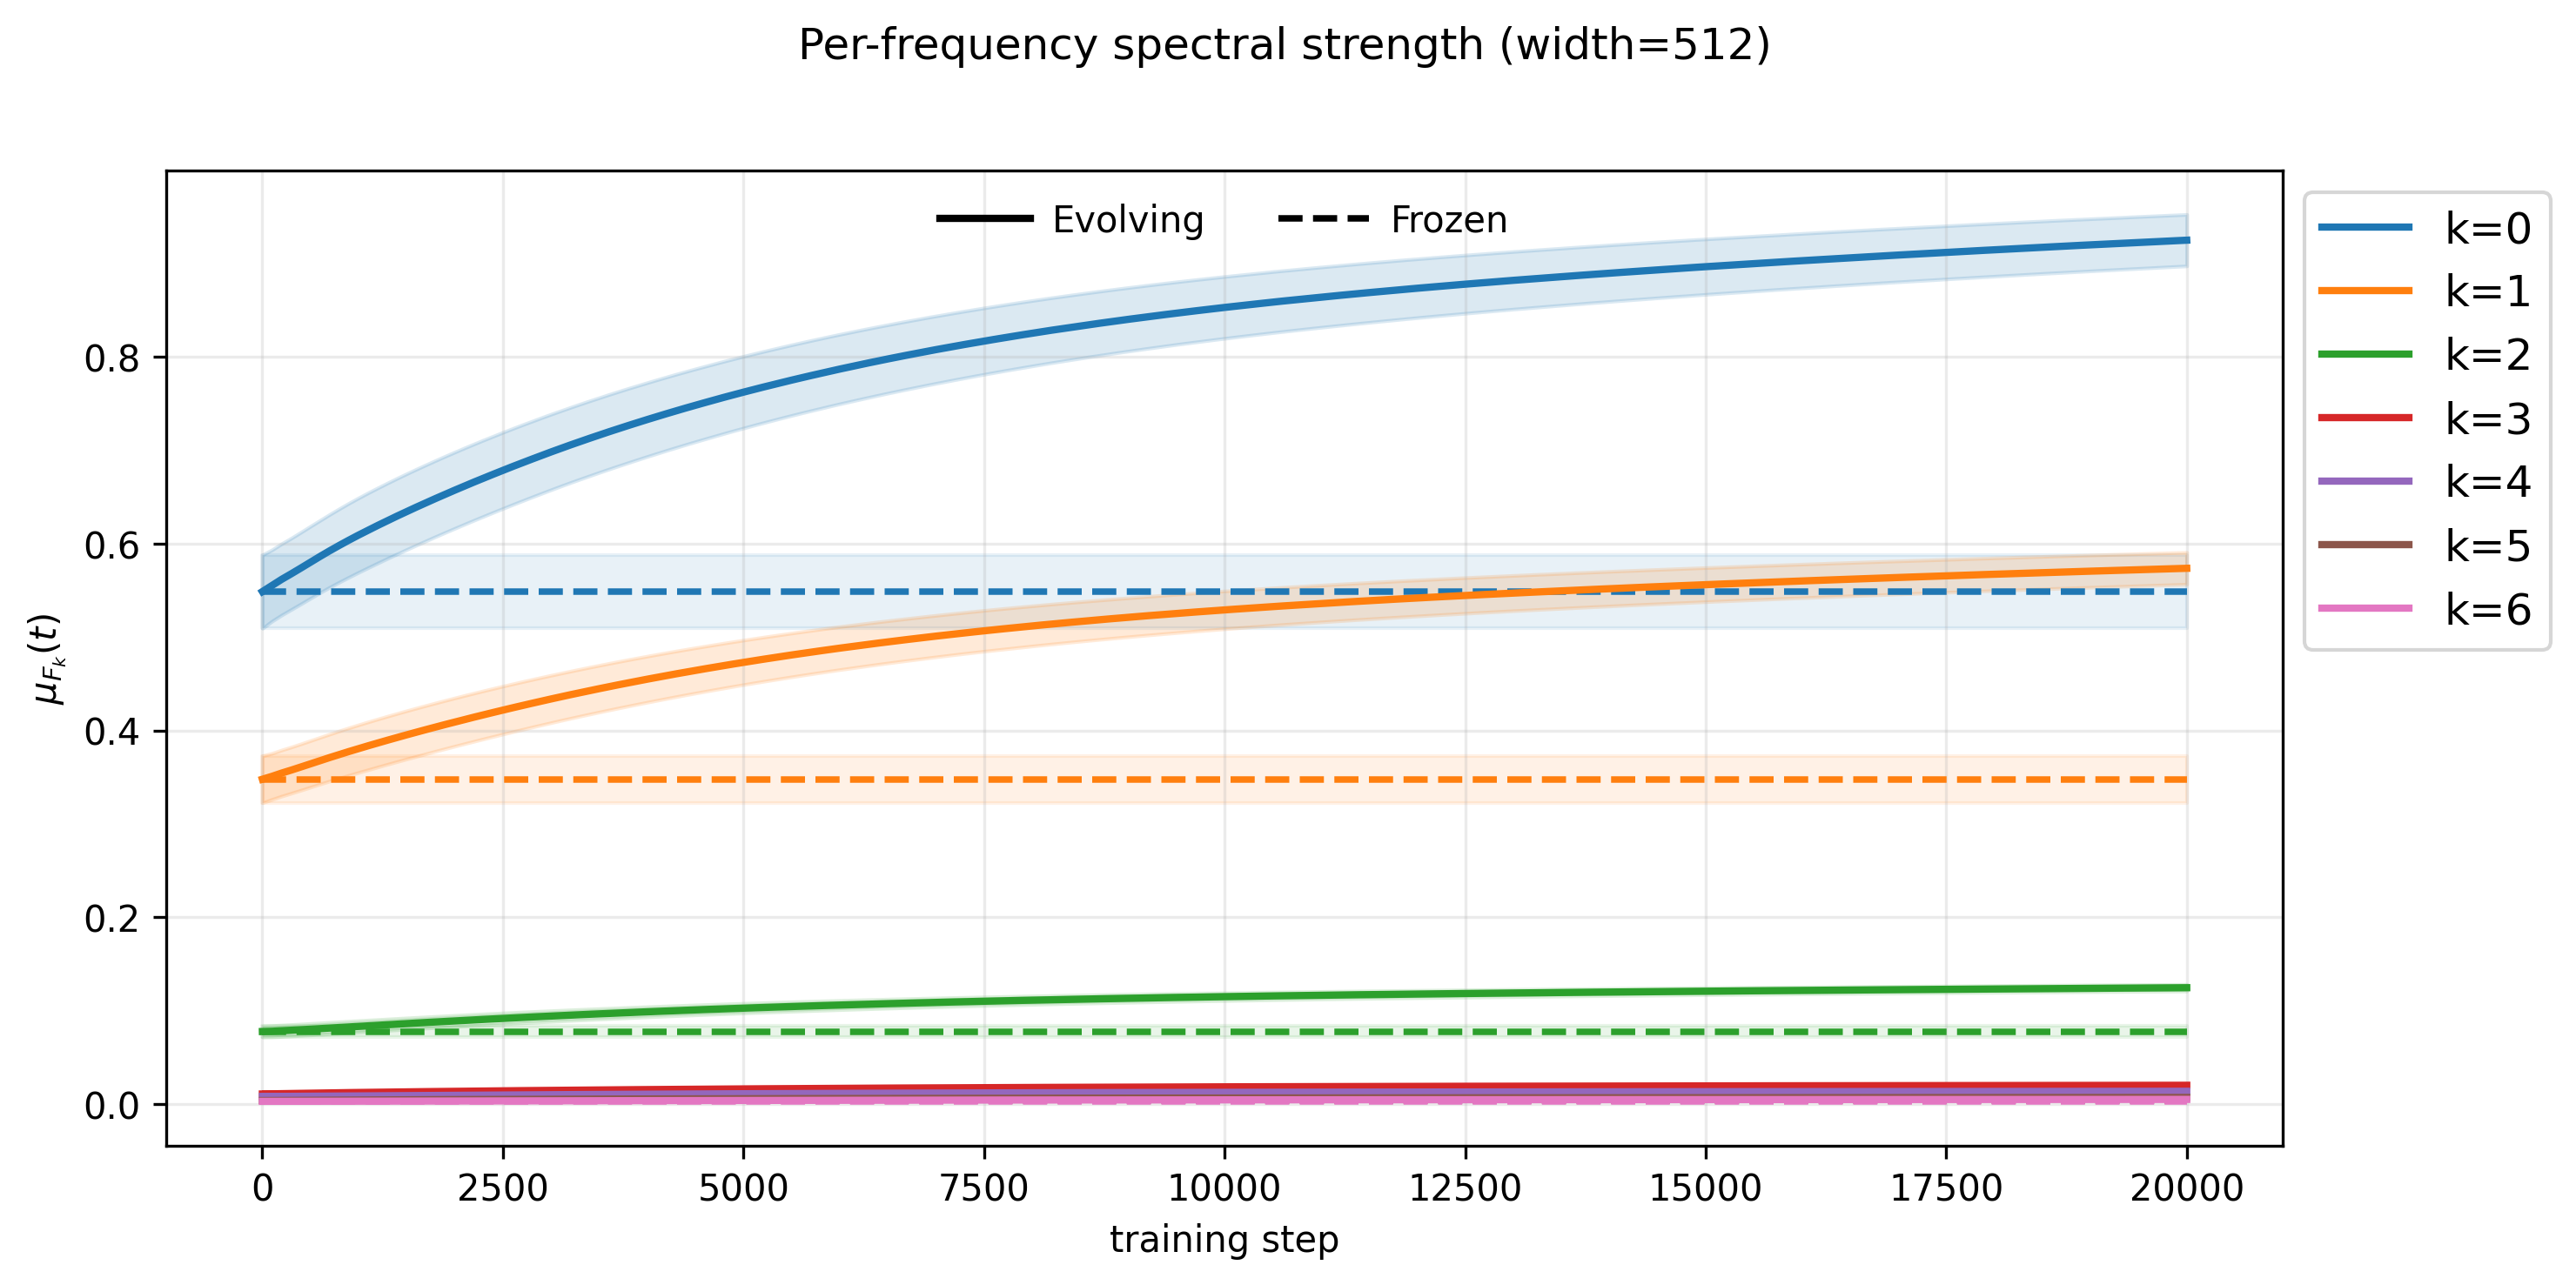
\includegraphics[width=\linewidth]{images/finite_width_evolving_results/spectral_strength_by_freq_w512.png}
		\caption{Per-frequency spectral strength.}
	\end{subfigure}

	\caption{Joint diagnostics for the evolving finite-width tangent kernel at
		width \(512\).}
	\label{fig:evolving-joint-w512}
\end{figure}

\begin{figure}[!htbp]
	\centering

	\begin{subfigure}[t]{\textwidth}
		\centering
		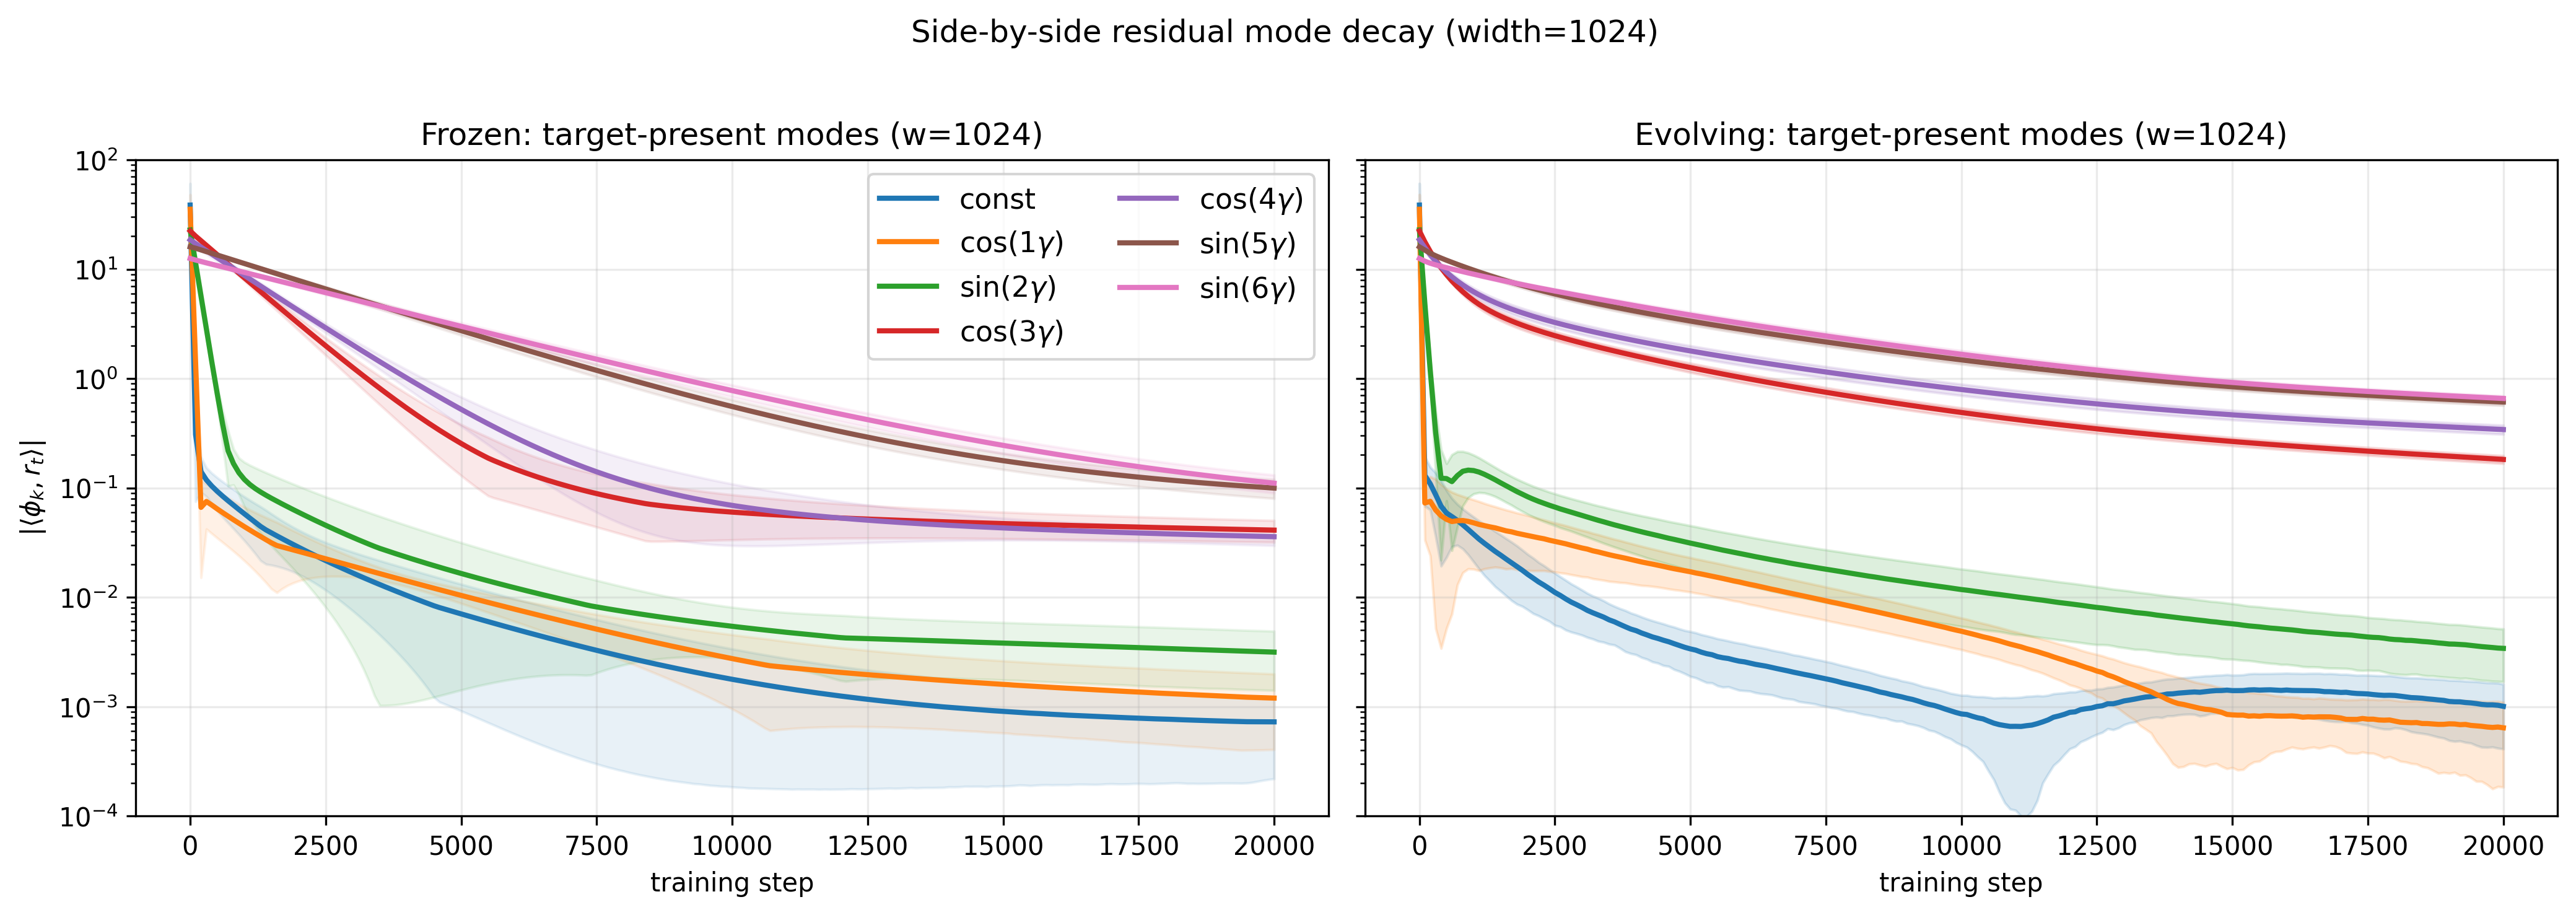
\includegraphics[width=\linewidth]{images/finite_width_evolving_results/side_by_side_residual_decay_w1024.png}
		\caption{Mode-wise residual decay.}
	\end{subfigure}

	\vspace{0.8em}

	\begin{subfigure}[t]{\textwidth}
		\centering
		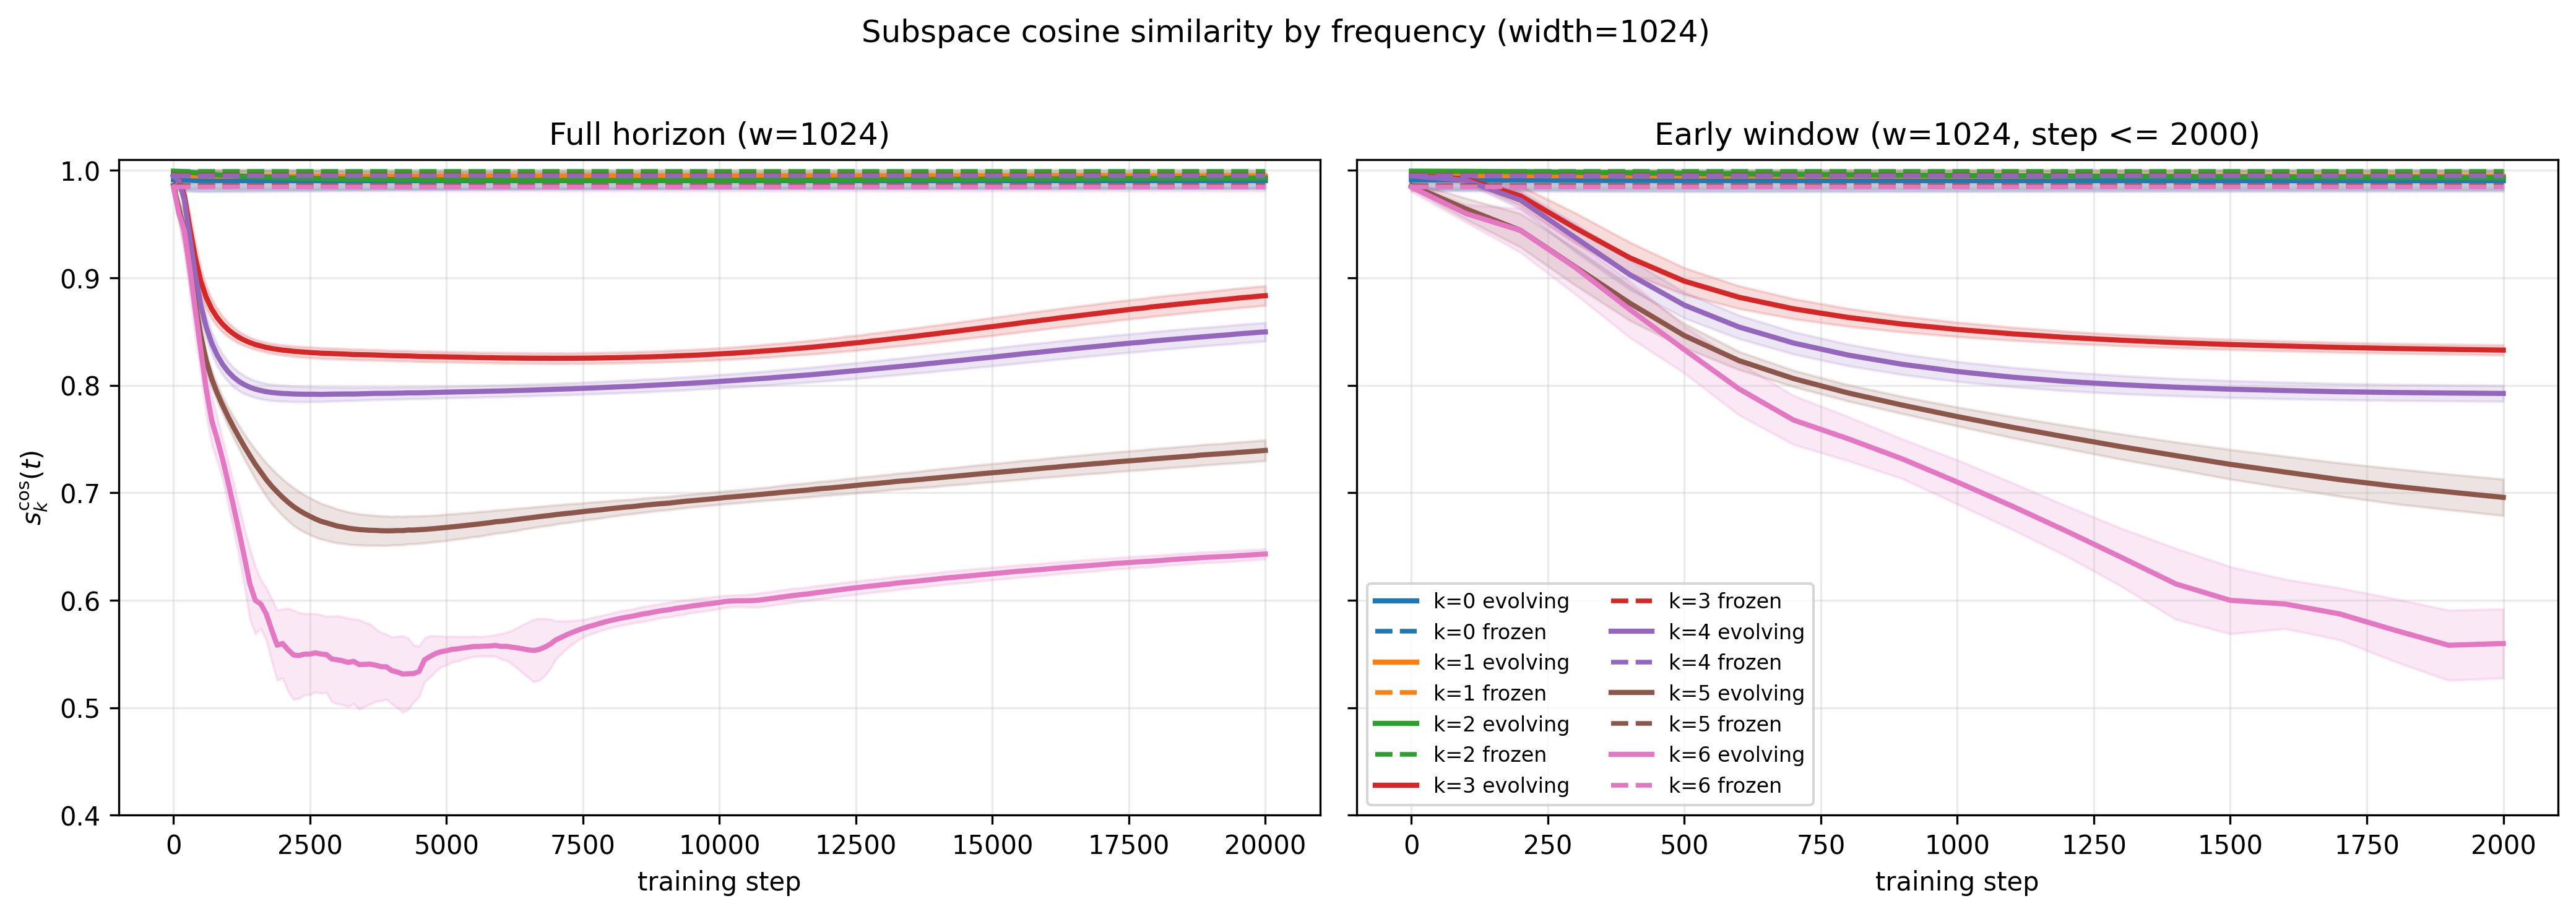
\includegraphics[width=\linewidth]{images/finite_width_evolving_results/rms_cos_alignment_by_freq_w1024.png}
		\caption{Subspace cosine similarity.}
	\end{subfigure}

	\vspace{0.8em}

	\begin{subfigure}[t]{\textwidth}
		\centering
		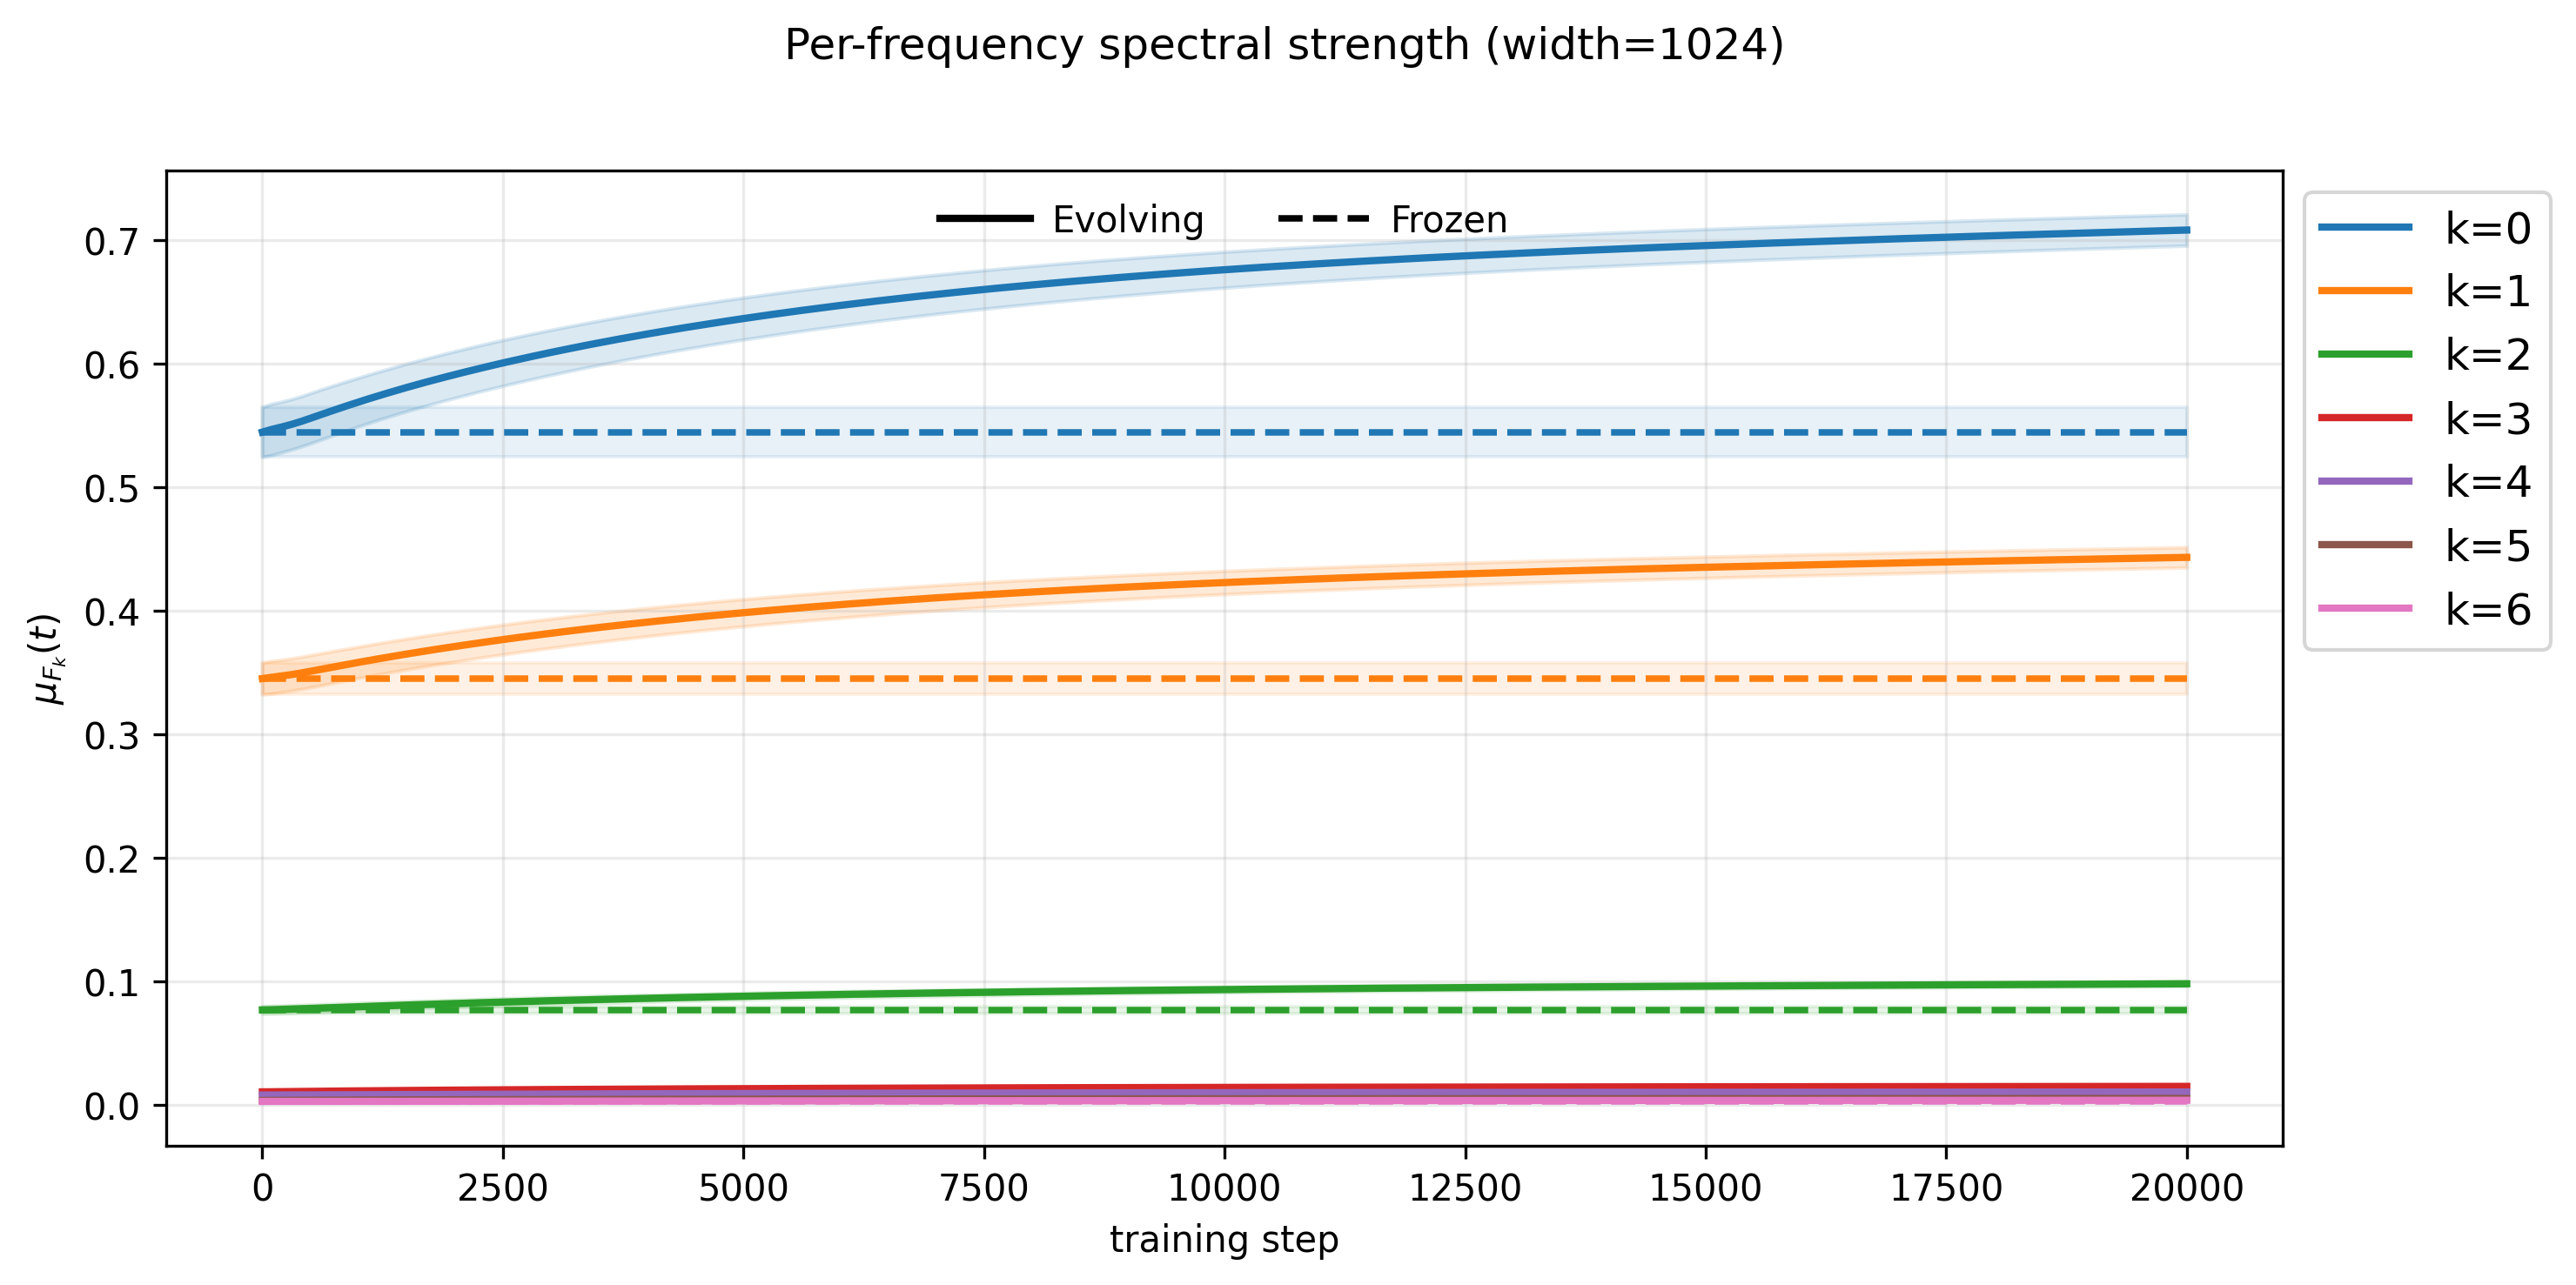
\includegraphics[width=\linewidth]{images/finite_width_evolving_results/spectral_strength_by_freq_w1024.png}
		\caption{Per-frequency spectral strength.}
	\end{subfigure}

	\caption{Joint diagnostics for the evolving finite-width tangent kernel at
		width \(1024\).}
	\label{fig:evolving-joint-w1024}
\end{figure}

Figures~\ref{fig:evolving-joint-w128}--\ref{fig:evolving-joint-w1024} show
three recurring trends. First, the mode-wise residual plots show that the early
training dynamics still largely follows the frequency ordering: lower-frequency
components decay before higher-frequency components. Kernel evolution does not
remove this ordering, but changes the relative decay rates within the retained
target modes. At widths \(128\) and \(256\), the evolving dynamics give
smaller final residuals for several low and intermediate modes, including the
constant mode, \(\cos(\varphi)\), \(\sin(2\varphi)\), \(\cos(3\varphi)\), and
\(\cos(4\varphi)\). At width \(512\), this advantage is less uniform. At width
\(1024\), the frozen dynamics are better on several components with the largest
remaining residual amplitudes, including \(\cos(3\varphi)\),
\(\cos(4\varphi)\), \(\sin(5\varphi)\), and \(\sin(6\varphi)\). Since the
least-squares objective is quadratic in the residual, these larger remaining
components have the greatest effect on the final loss.

Second, the subspace cosine similarity plots show that kernel evolution does
not improve Fourier alignment. The low-frequency subspaces, especially
\(k=0\), \(k=1\), and to a lesser extent \(k=2\), remain close to their Fourier
subspaces during training. In contrast, several higher-frequency subspaces lose
alignment early in training and only partially recover later. The frozen
alignment improves with width, as expected from the frozen finite-width results.
The evolving alignment, however, reaches a similar range across widths for some
higher frequencies. Thus, at larger width, the evolving kernel can move farther
away from the better-aligned initialization, even though the low-frequency
subspaces remain relatively stable.

Third, the spectral-strength plots show that the largest change in operator
strength occurs precisely in the low-frequency blocks that remain well aligned.
At width \(128\), the average strength in the constant block and the first
frequency increases by a large factor during training, with a smaller increase
for \(k=2\). The same effect is present at width \(256\), weaker at width
\(512\), and much smaller at width \(1024\). The higher-frequency blocks remain
weak in comparison and do not show the same increase in strength.

Taken together, these plots suggest that the small-width benefit of kernel
evolution is not caused by better preservation of Fourier geometry. The
alignment either stays similar for the lowest frequencies or worsens for higher
frequencies. The more visible effect is that kernel evolution increases the
operator strength in the low-frequency blocks that are already well aligned
with the Fourier subspaces. At small width, this extra low-frequency strength
can outweigh the loss of alignment elsewhere. At large width, the frozen kernel
already has good Fourier structure, and the additional strength gained from
kernel evolution is smaller, so the evolving dynamics no longer gives a clear
advantage.

\subsection{Width dependence of tangent-kernel drift}
\label{subsec:results-evolving-block-drift}

The previous plots compare the consequences of frozen and evolving dynamics.
We now measure the kernel movement directly. Recall from
Section~\ref{sec:finite-width-evolving-kernel-methodology} that
\[
	C_t^{(K)}=P_KT_t^{(m)}P_K
\]
denotes the low-frequency block of the finite-width tangent operator. We measure
its drift from initialization by
\[
	\|C_t^{(K)}-C_0^{(K)}\|_F .
\]

\begin{figure}[!htbp]
	\centering
	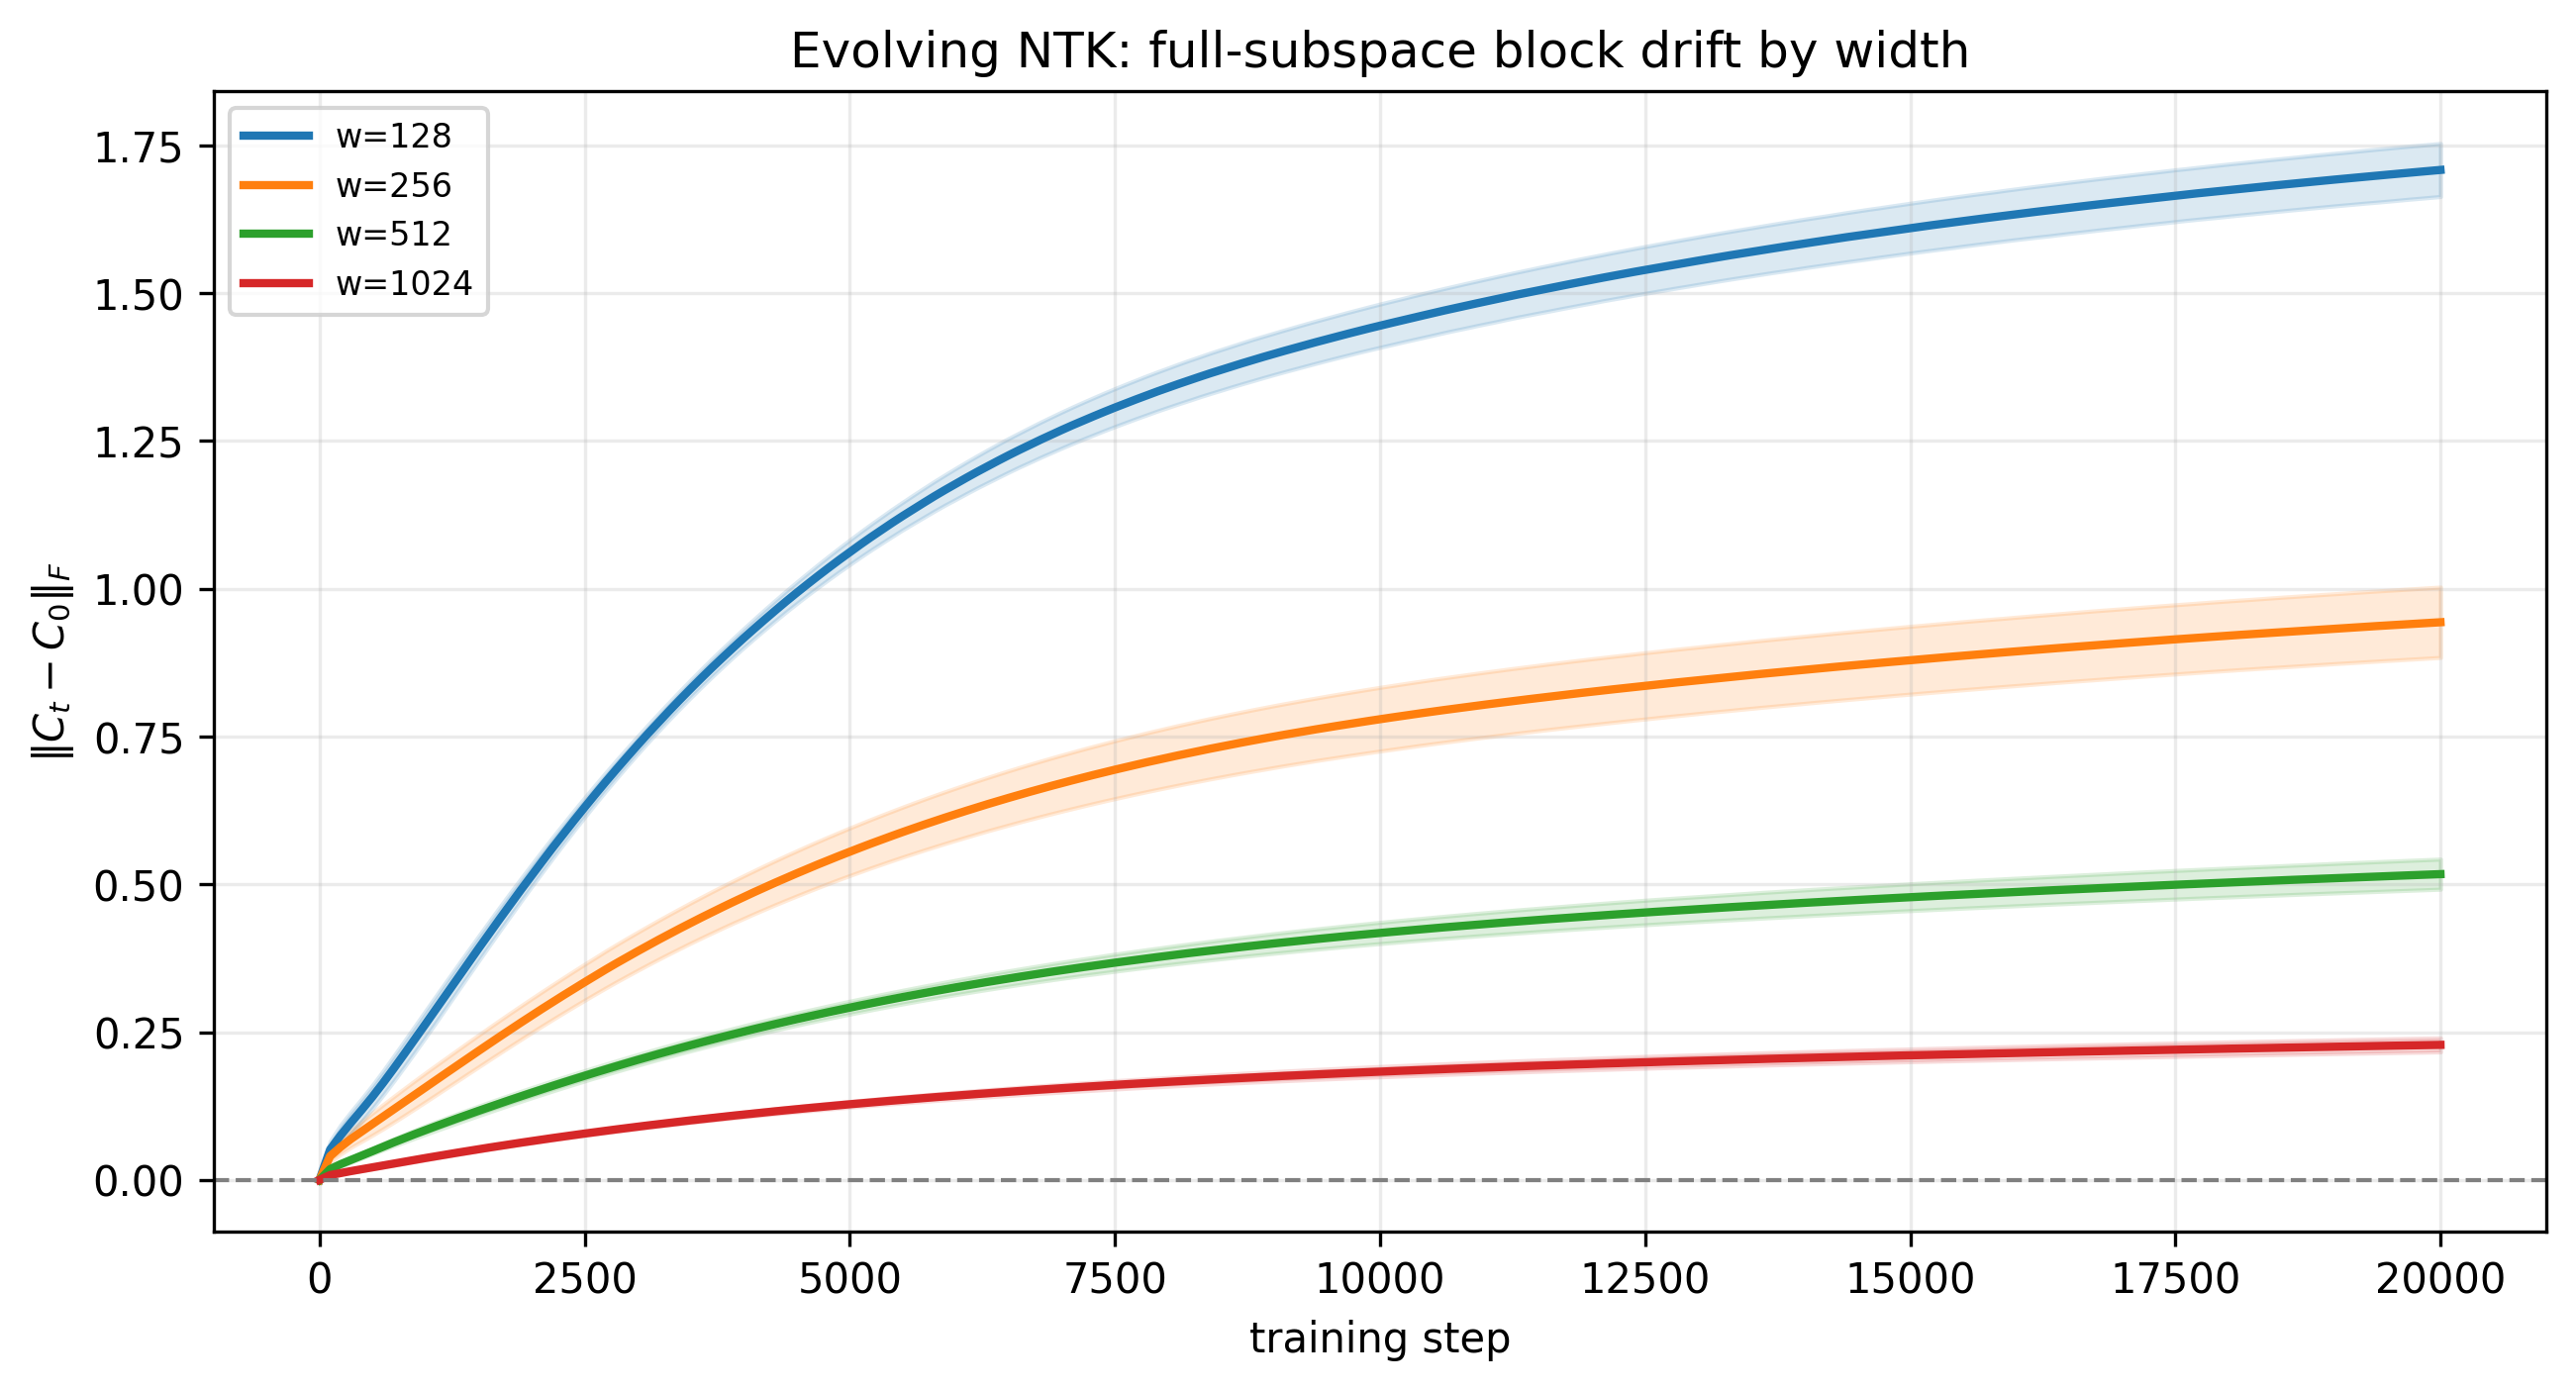
\includegraphics[width=0.9\textwidth]{images/finite_width_evolving_results/full_subspace_block_drift_fro_Ct_minus_C0_by_width_full.png}
	\caption{Drift of the projected evolving tangent-kernel block across widths,
	measured by \(\|C_t^{(K)}-C_0^{(K)}\|_F\). The low-frequency block changes
	substantially at small width and much less at larger width.}
	\label{fig:results-evolving-block-drift}
\end{figure}

Figure~\ref{fig:results-evolving-block-drift} shows the drift of the projected
low-frequency tangent block during training. The drift is largest at widths
\(128\) and \(256\), and becomes much smaller at widths \(512\) and \(1024\).
Thus, in these experiments, the finite-width tangent kernel moves less as the
width increases.

This is consistent with the NTK regime, where increasing width makes the
training dynamics closer to the linearized dynamics around initialization and
the tangent kernel changes less during training
\citep{jacot2018ntk,lee2020wide,chizat2019lazytraining}. In the present
experiments, this also explains why the difference between frozen and evolving
dynamics are most visible at small width.

\subsection{Effect of target amplitudes on spectral strength}
\label{subsec:results-evolving-amplitude-variants}

The spectral-strength plots above suggest that the evolving tangent kernel
increases its strength mainly on the low-frequency blocks. One possible concern
is that this effect could be caused by the particular amplitudes in the target
function. In the original target, the lower-frequency components have larger
amplitudes than the higher-frequency components. To check whether the observed
spectral reweighting is tied to this choice, we repeat the evolving-kernel
experiment with two modified targets.

The three targets are
	{\footnotesize
		\begin{align}
			f_{\mathrm{orig}}(\gamma)
			 & =
			1.0
			+0.9\cos(\gamma)
			-0.8\sin(2\gamma)
			+0.7\cos(3\gamma)
			+0.6\cos(4\gamma)
			-0.5\sin(5\gamma)
			-0.4\sin(6\gamma),
			\label{eq:results-target-original}
			\\
			f_{\mathrm{eq}}(\gamma)
			 & =
			1.0
			+\cos(\gamma)
			-\sin(2\gamma)
			+\cos(3\gamma)
			+\cos(4\gamma)
			-\sin(5\gamma)
			-\sin(6\gamma),
			\label{eq:results-target-equalamp}
			\\
			f_{\mathrm{rev}}(\gamma)
			 & =
			0.4
			+0.5\cos(\gamma)
			-0.6\sin(2\gamma)
			+0.7\cos(3\gamma)
			+0.8\cos(4\gamma)
			-0.9\sin(5\gamma)
			-\sin(6\gamma).
			\label{eq:results-target-revamp}
		\end{align}
	}

The equal-amplitude target gives all active non-constant modes the same
amplitude. The reversed-amplitude target gives the largest amplitudes to the
higher-frequency modes.

\begin{figure}[!htbp]
	\centering
	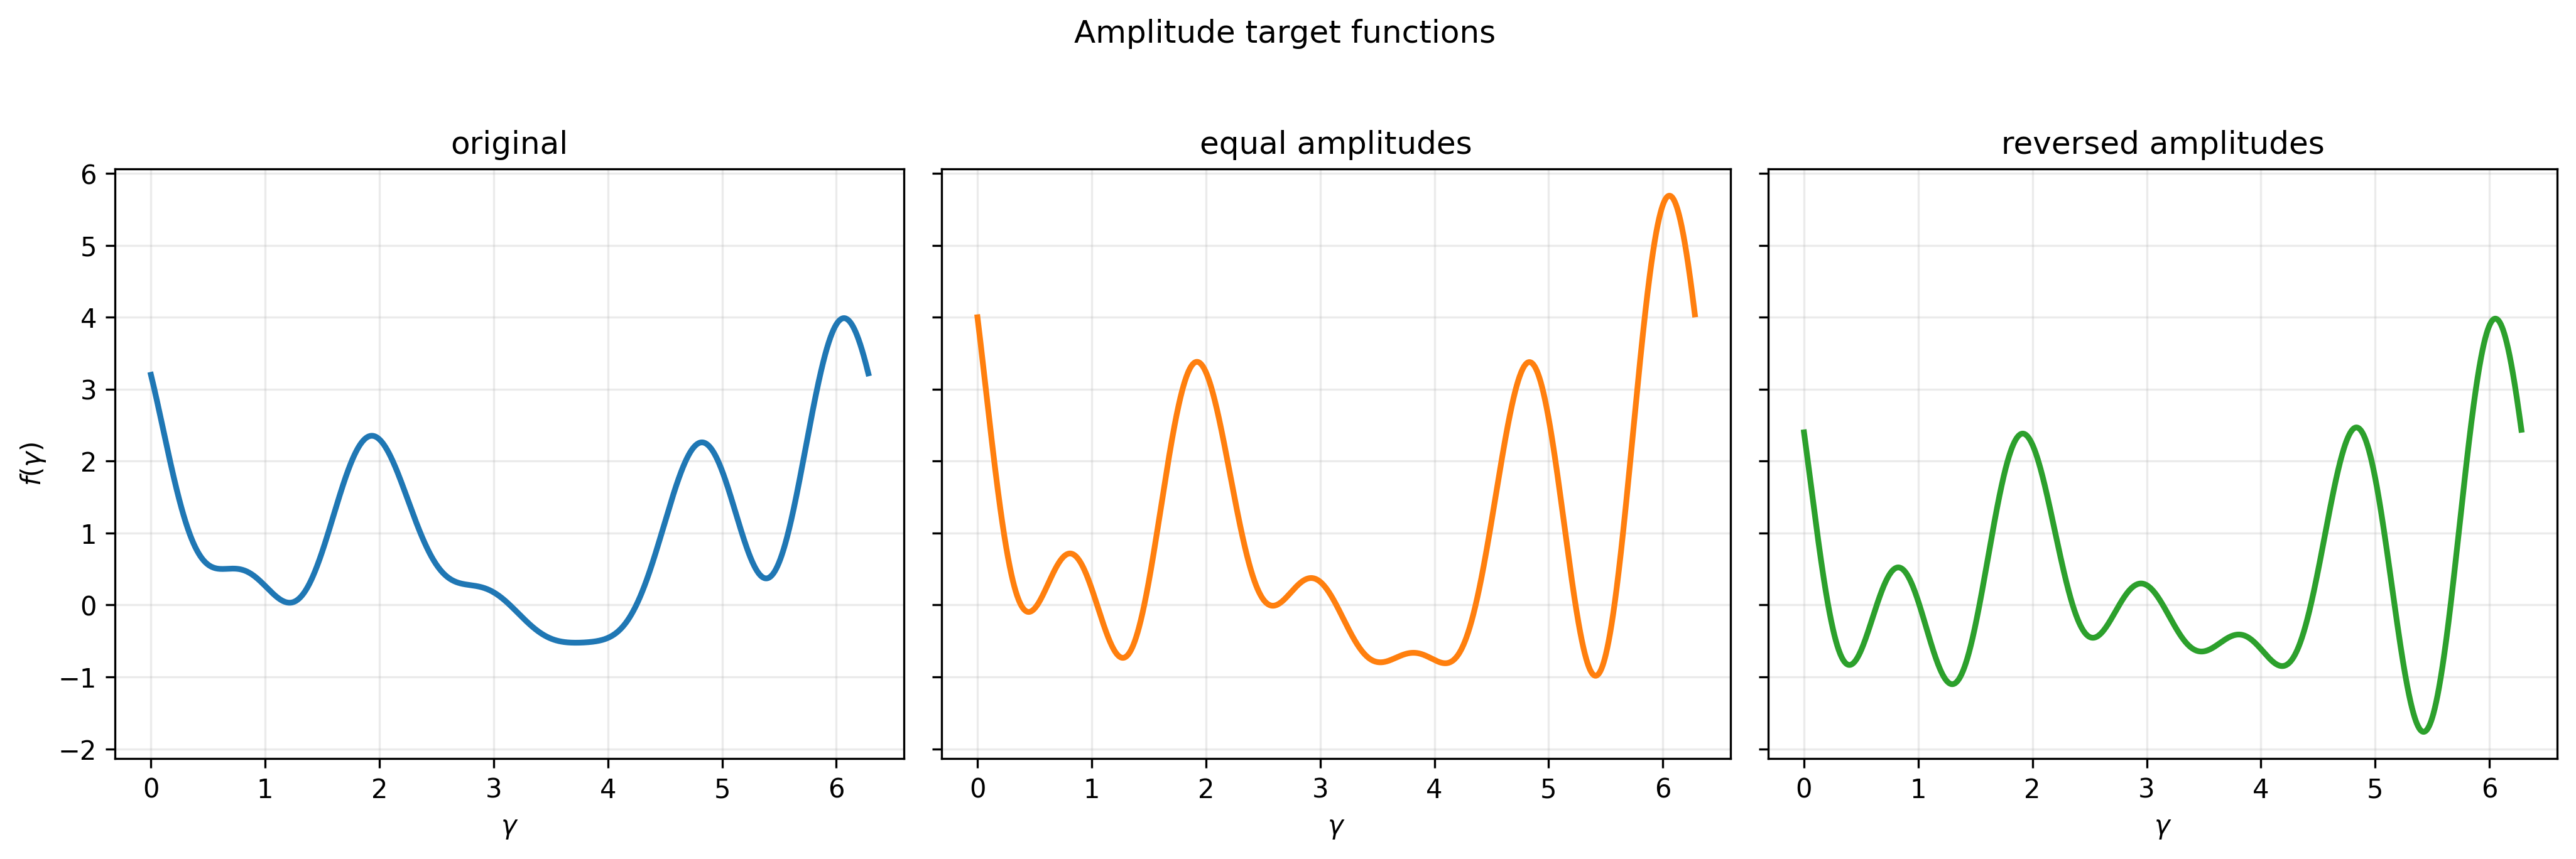
\includegraphics[width=\textwidth]{images/finite_width_evolving_results/amplitude_target_functions.png}
	\caption{Target functions used in the amplitude-variant experiments. The
		original target has larger amplitudes on lower frequencies, the
		equal-amplitude target assigns the same amplitude to all active
		non-constant modes, and the reversed-amplitude target gives larger
		amplitudes to higher frequencies.}
	\label{fig:results-amplitude-target-functions}
\end{figure}

\begin{figure}[!htbp]
	\centering

	\begin{subfigure}[t]{0.48\textwidth}
		\centering
		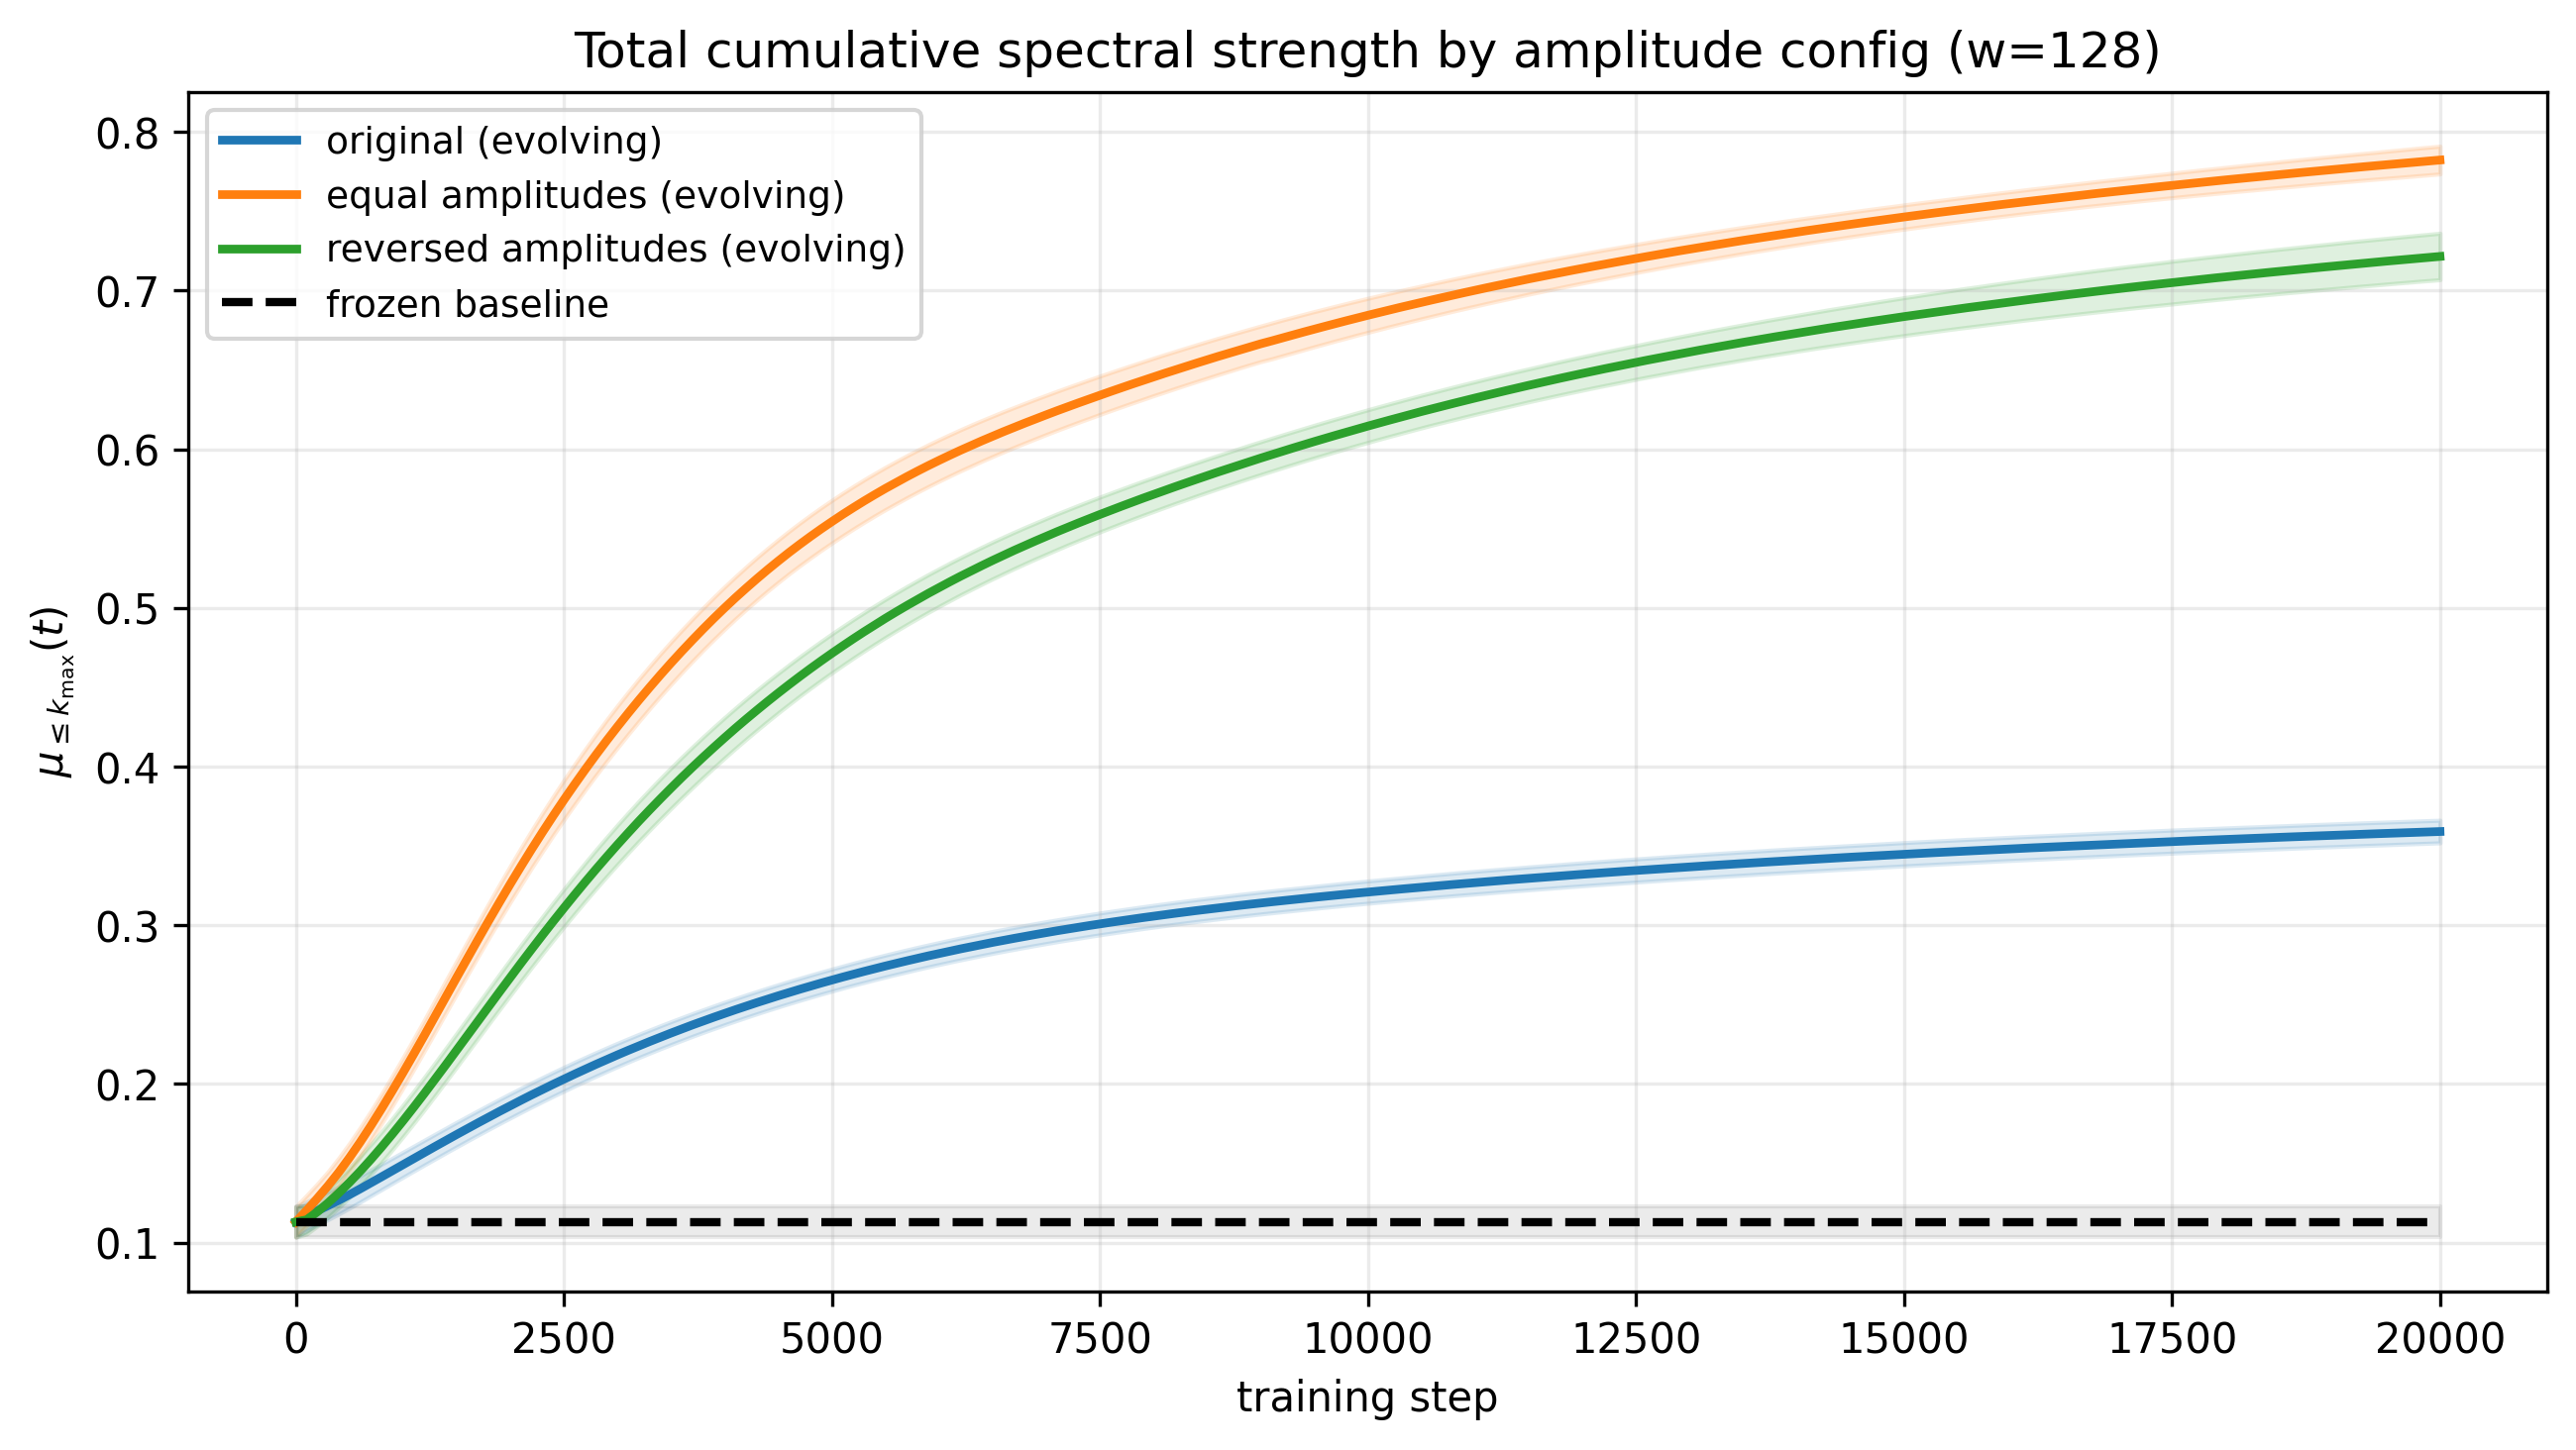
\includegraphics[width=\linewidth]{images/finite_width_evolving_results/total_cumulative_mu_amp_configs_w128.png}
		\caption{\(w=128\).}
	\end{subfigure}
	\hfill
	\begin{subfigure}[t]{0.48\textwidth}
		\centering
		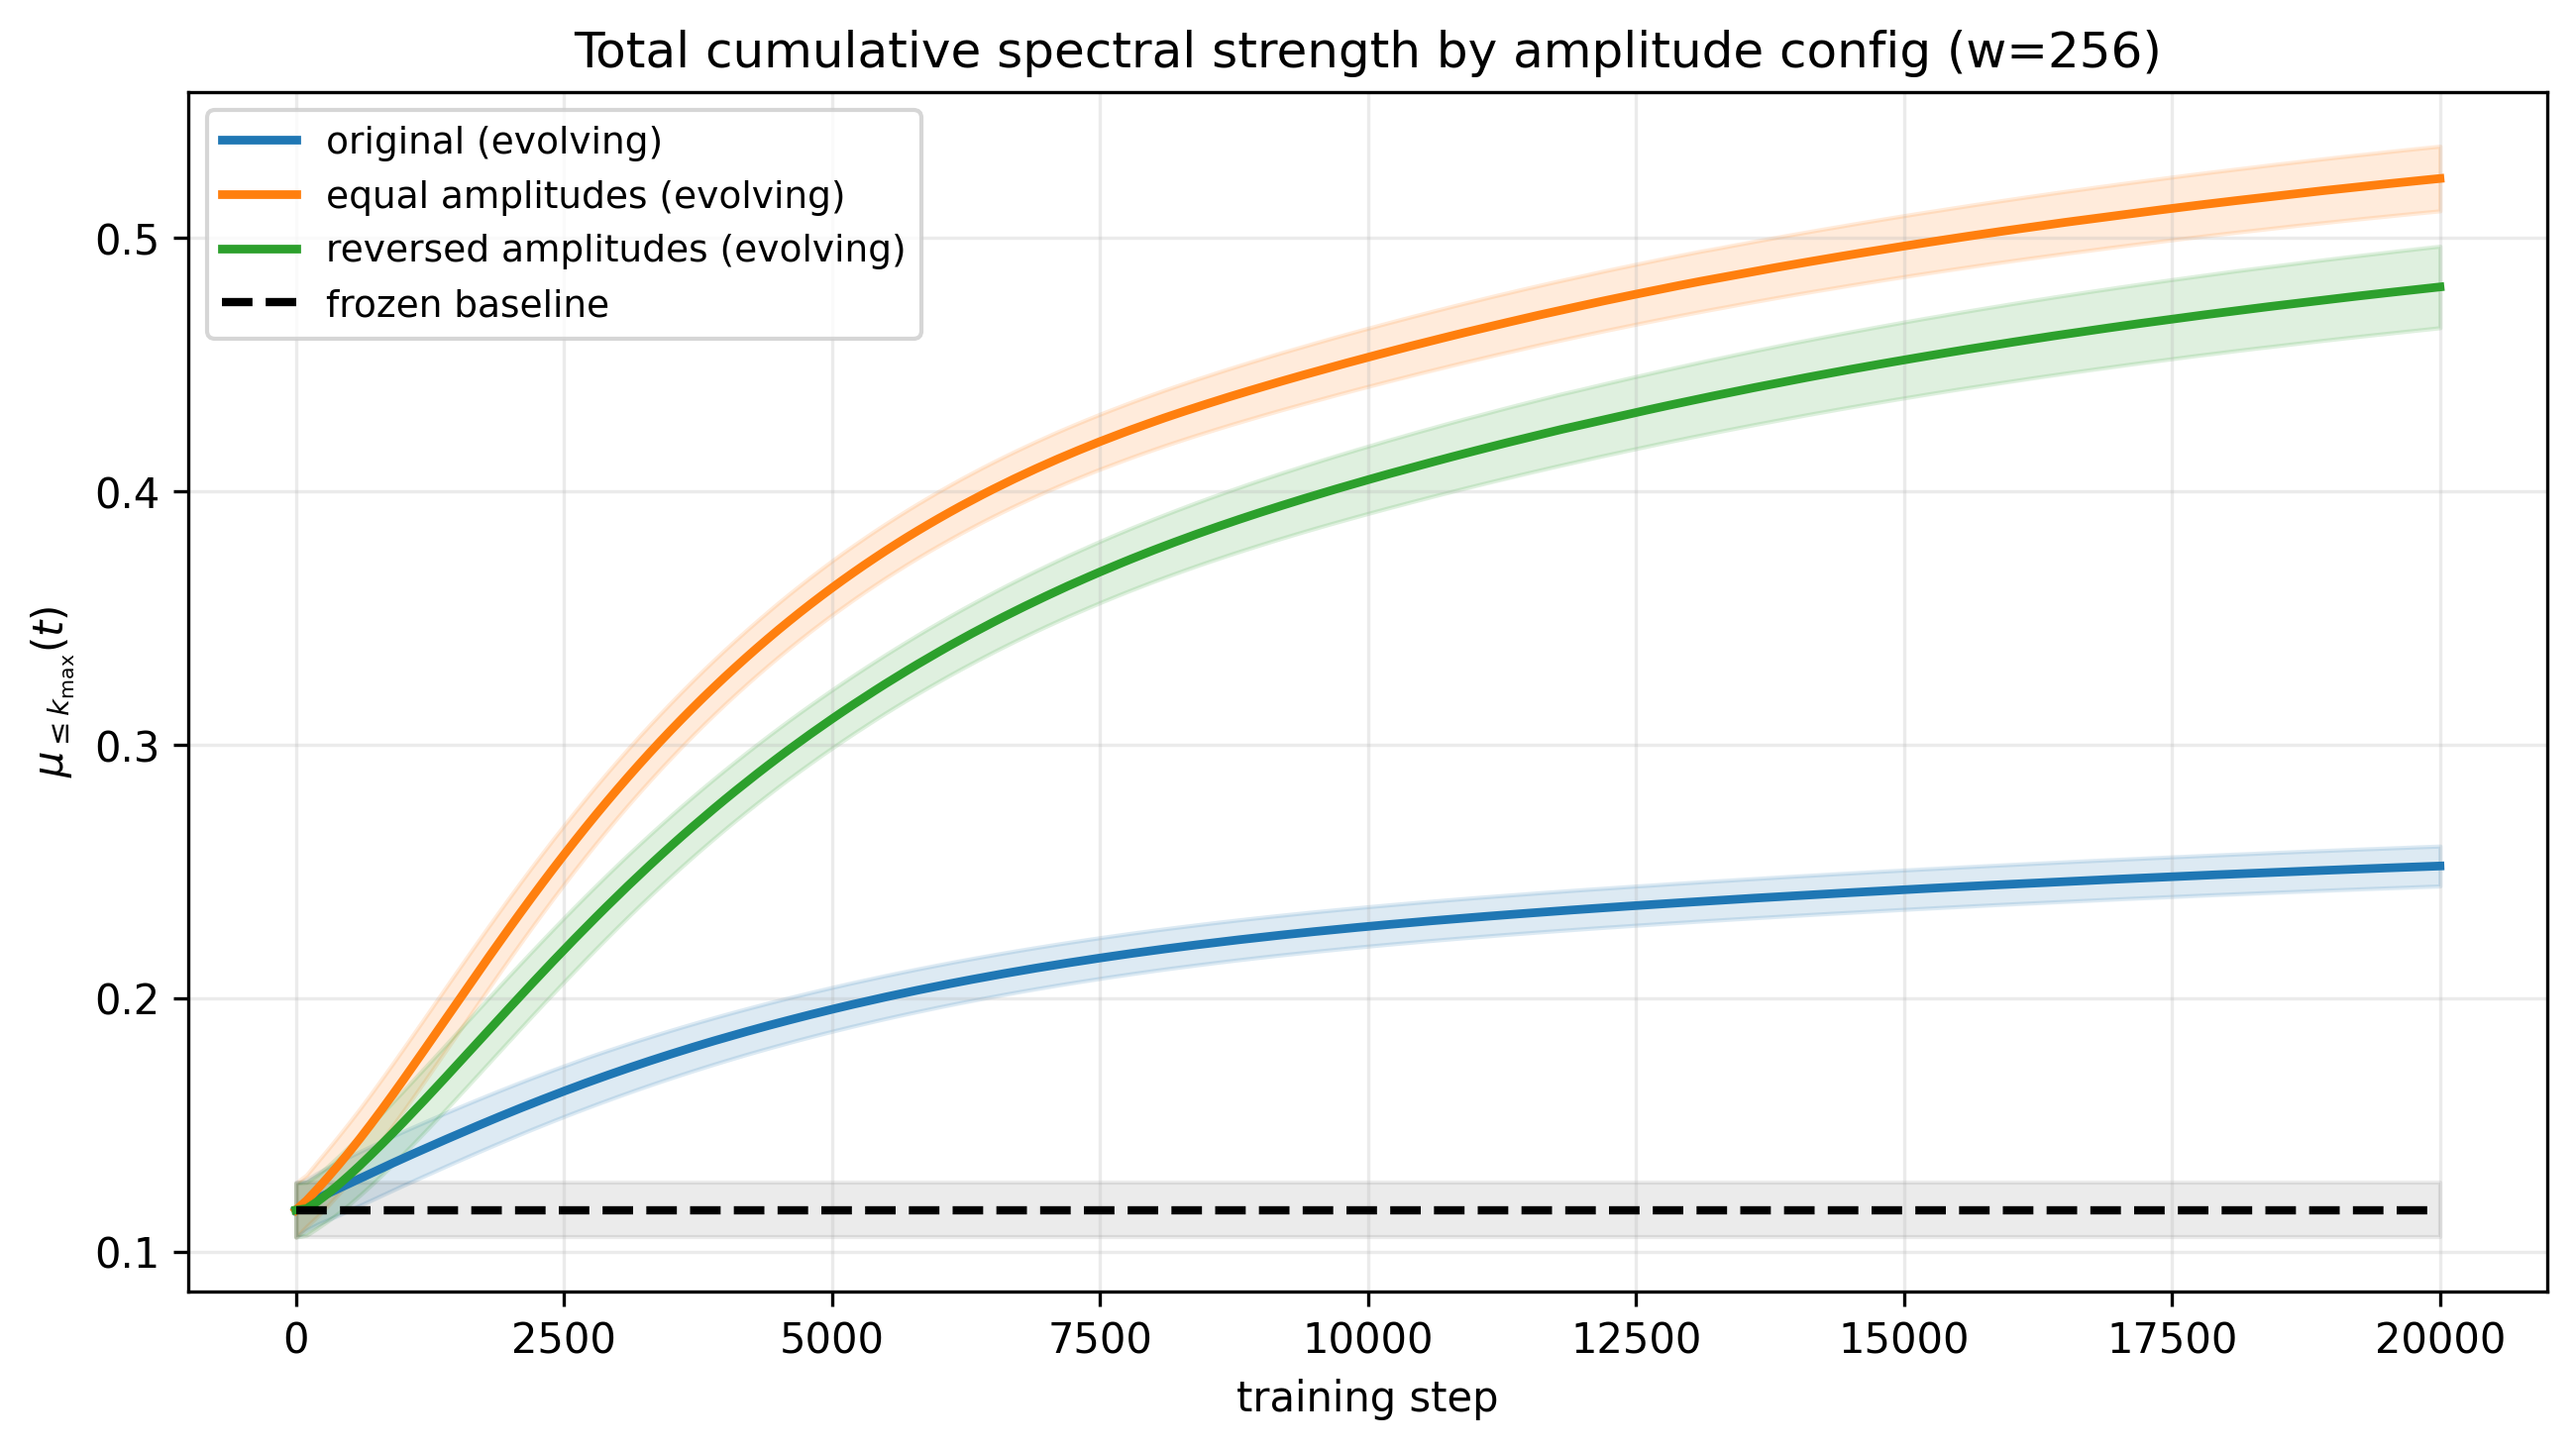
\includegraphics[width=\linewidth]{images/finite_width_evolving_results/total_cumulative_mu_amp_configs_w256.png}
		\caption{\(w=256\).}
	\end{subfigure}

	\vspace{0.8em}

	\begin{subfigure}[t]{0.48\textwidth}
		\centering
		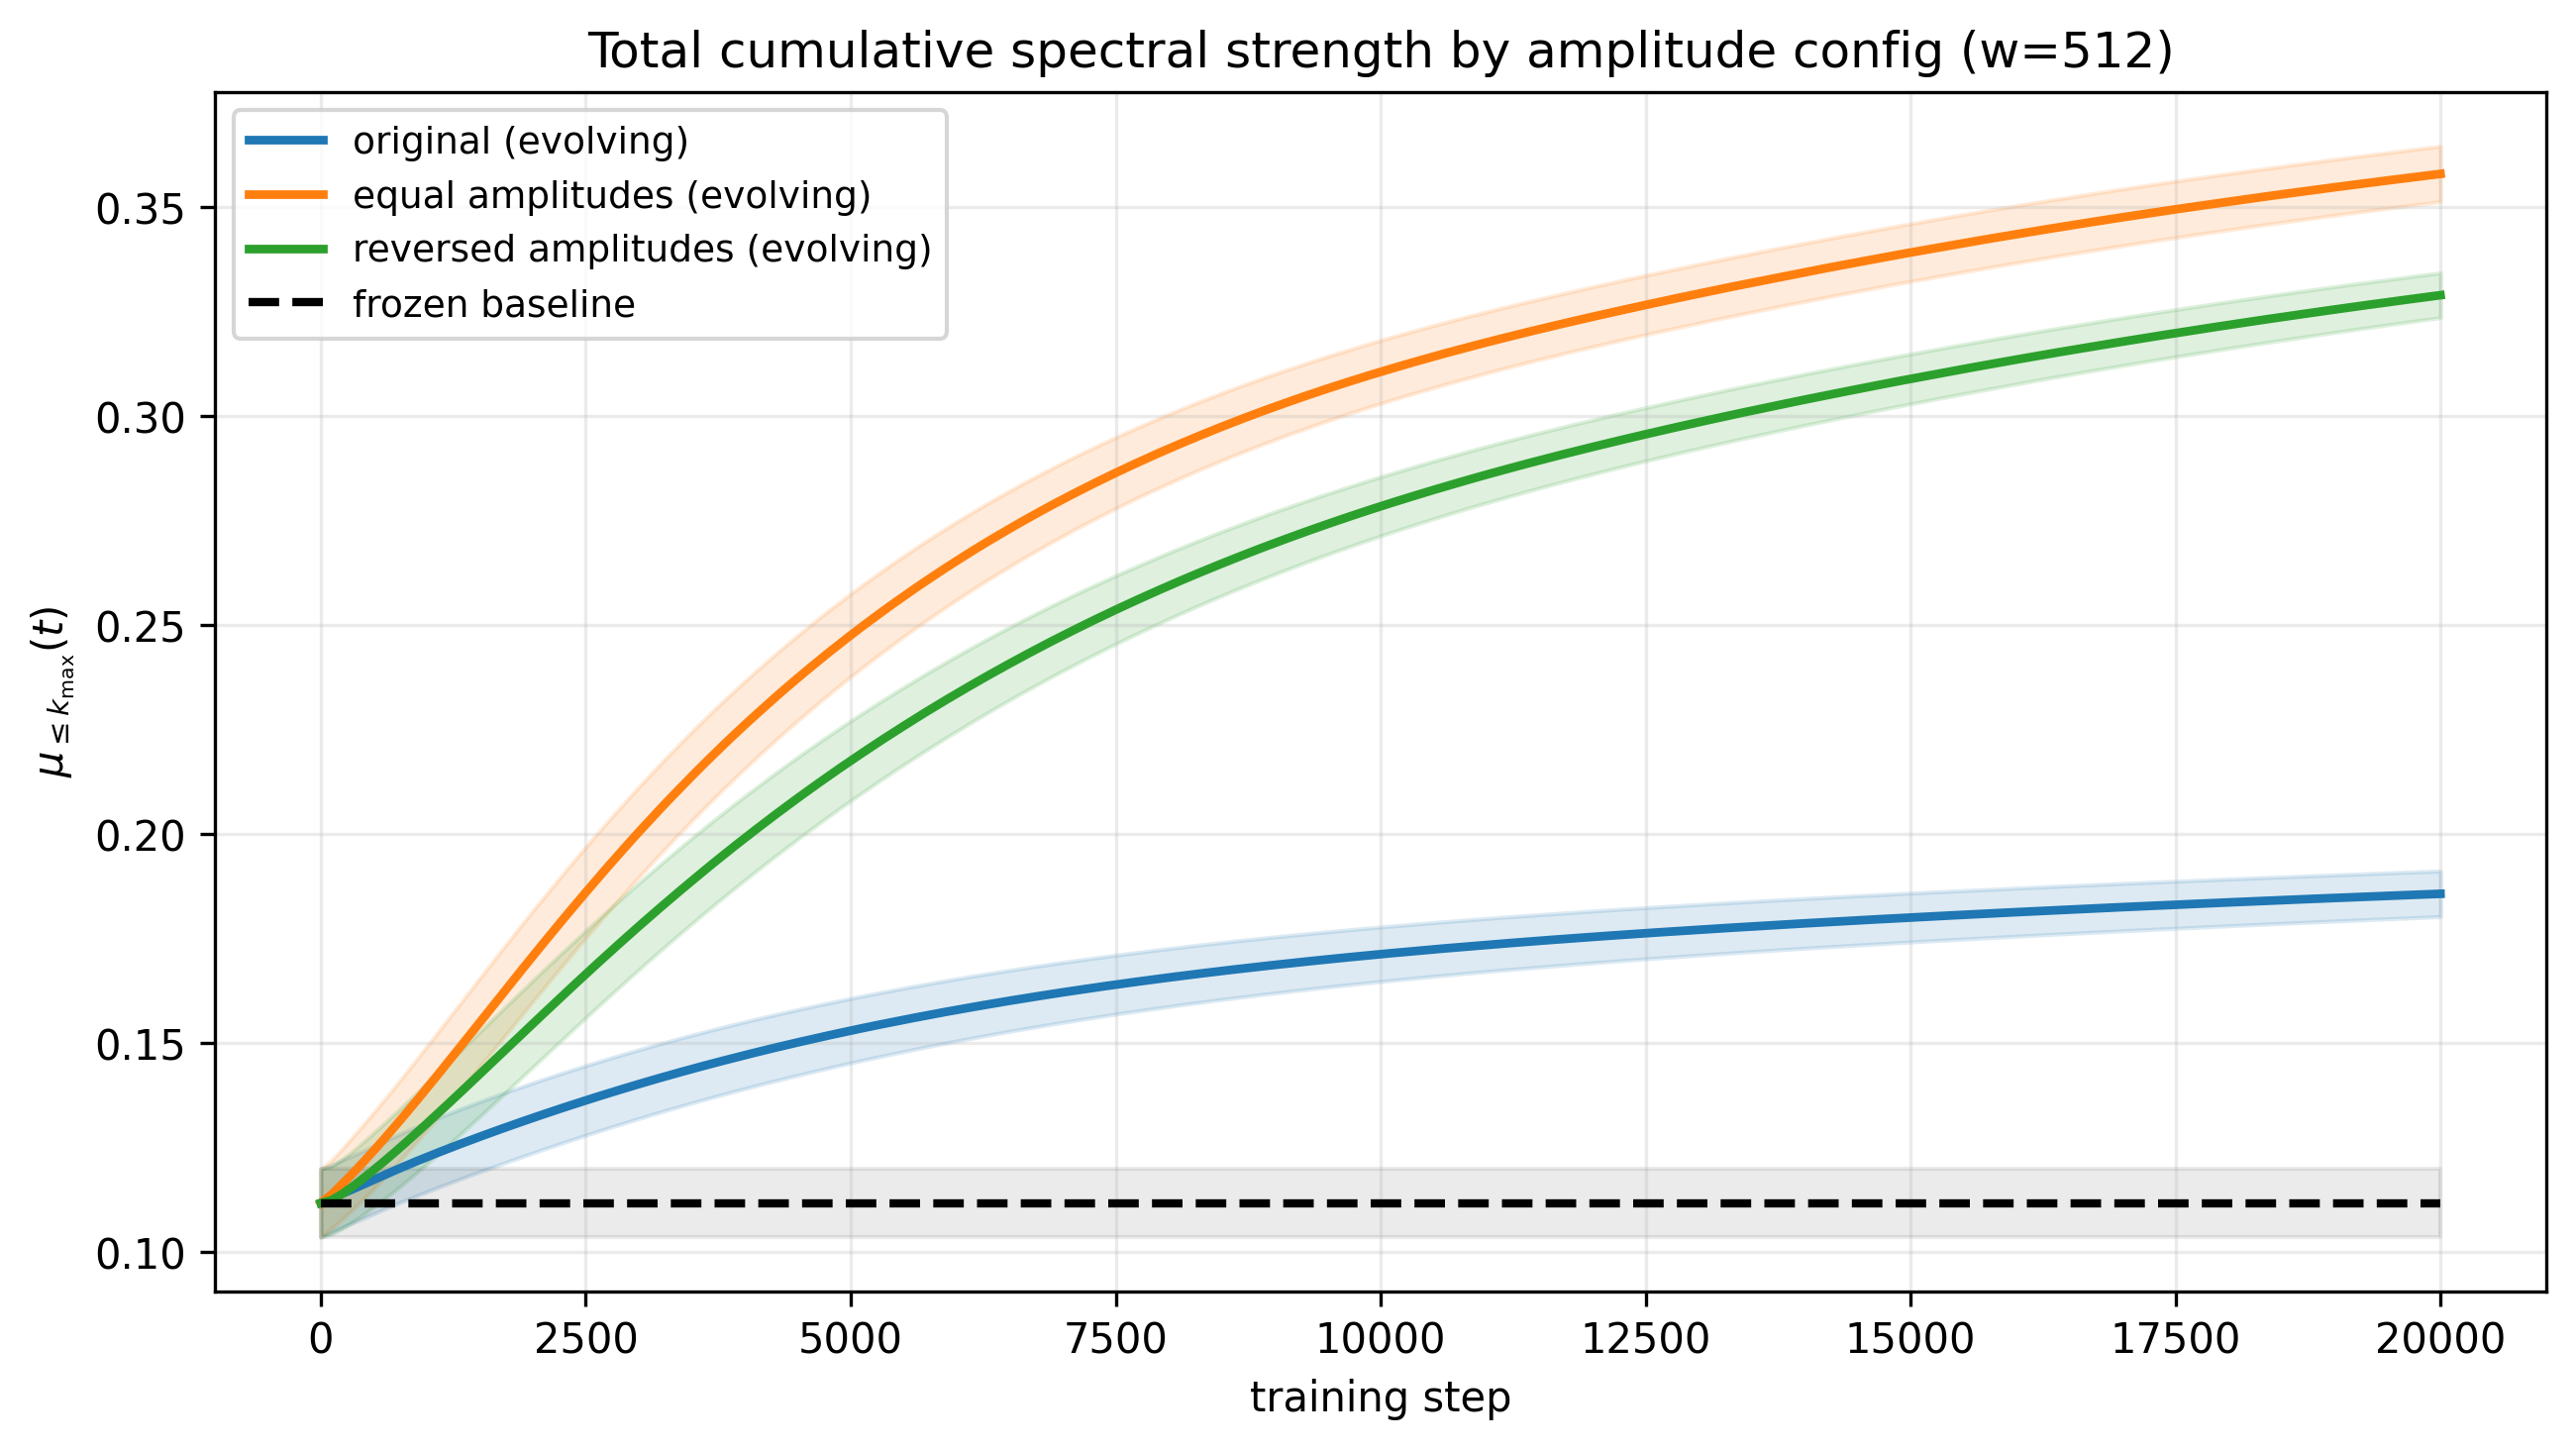
\includegraphics[width=\linewidth]{images/finite_width_evolving_results/total_cumulative_mu_amp_configs_w512.png}
		\caption{\(w=512\).}
	\end{subfigure}
	\hfill
	\begin{subfigure}[t]{0.48\textwidth}
		\centering
		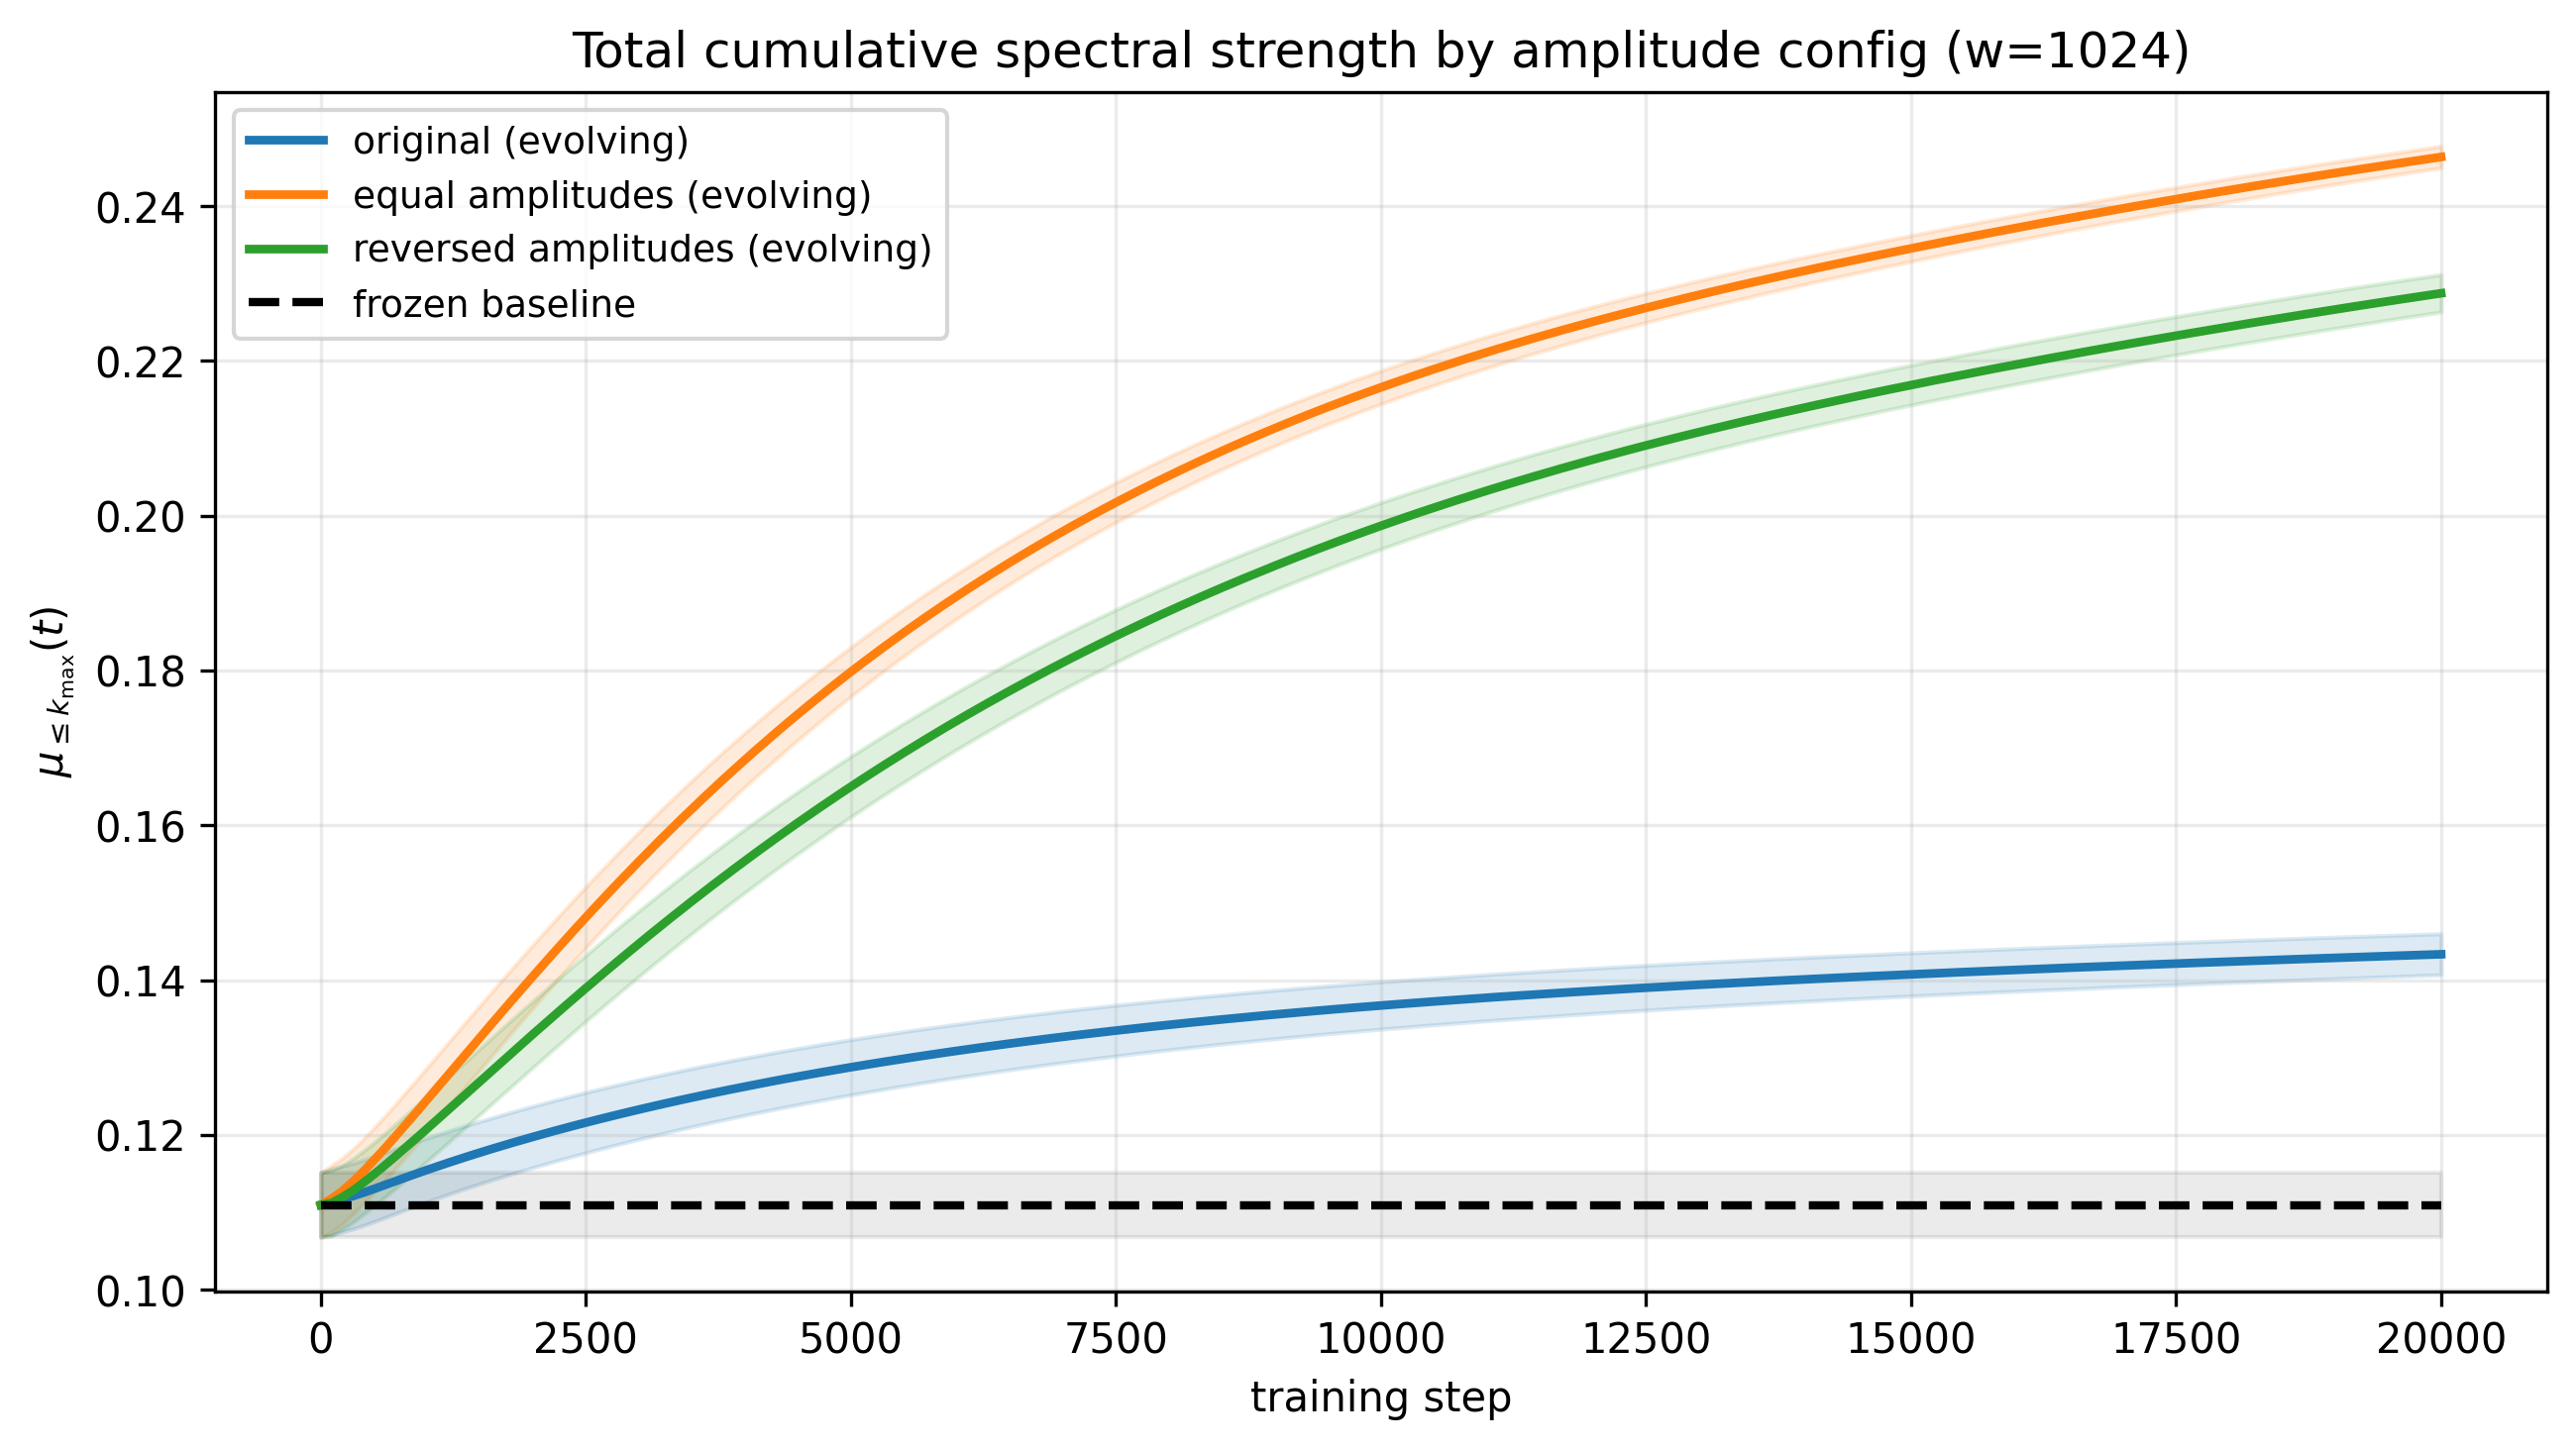
\includegraphics[width=\linewidth]{images/finite_width_evolving_results/total_cumulative_mu_amp_configs_w1024.png}
		\caption{\(w=1024\).}
	\end{subfigure}

	\caption{Cumulative low-frequency spectral strength under different target
		amplitude choices. The dashed line shows the frozen baseline, while the
		solid curves show the evolving tangent kernel for the original,
		equal-amplitude, and reversed-amplitude targets.}
	\label{fig:results-cumulative-strength-amplitude-variants}
\end{figure}

Figure~\ref{fig:results-cumulative-strength-amplitude-variants} shows that the
increase in cumulative spectral strength is not specific to the original target
amplitudes. For all widths, the evolving tangent kernel increases the average
strength on the retained low-frequency block relative to the frozen baseline.
This increase is largest for the equal-amplitude target, smaller but still clear
for the reversed-amplitude target, and weakest for the original target.

The effect also decreases with width. At width \(128\), all evolving curves move
well above the frozen baseline. At width \(1024\), the same ordering is still
visible, but the increase is smaller. Thus, the low-frequency strength increase
persists across all three amplitude choices. It is not only a consequence of
the original target assigning larger amplitudes to lower frequencies: the
increase is also present when all non-constant modes have equal amplitudes, and
when the larger amplitudes are assigned to higher frequencies.

The ordering across targets is also worth noting. In these experiments, the
equal-amplitude target produces the largest increase, the reversed-amplitude
target produces a smaller but still clear increase, and the original target
produces the weakest increase. In particular, the reversed-amplitude target
still produces a larger low-frequency strength increase than the original
target, despite putting larger amplitudes on higher-frequency modes.

\section{Summary of results}
\label{sec:results-summary}

This chapter tested how the idealized infinite-width, infinite-data spectral
bias picture changes under realistic constraints in a controlled fashion.
Throughout these analyses, the primary comparisons are made on the retained
low-frequency subspace $\mathcal{H}_K$, which contains the constant mode and
the first $K$ non-zero Fourier frequencies.

The core findings are:

\begin{itemize}
	\item \textbf{Ideal continuum setting:} Under the limiting NTK, each
	      Fourier component evolves independently. Lower frequencies possess larger
	      eigenvalues and decay faster. Crucially, the architecture dictates the
	      spectrum: odd modes $k \ge 3$ only receive non-zero eigenvalues if the
	      network includes a trainable hidden bias.

	\item \textbf{Finite sampling:} Replacing the continuous measure with $n$
	      discrete samples destroys exact Fourier diagonalization. However, on
	      $\mathcal{H}_K$, the sampled operator deviates from the ideal Fourier
	      prediction by an error of just $O(n^{-1/2})$ (with fixed confidence, up to
	      logarithmic factors). The corrected finite-sample eigenvalues (see
	      ~\ref{prop:results-expectation-H}) accurately predict the dominant
	      early-time residual decay.

	\item \textbf{Frozen finite width:} When fixing a finite-width ($m$)
	      tangent kernel at initialization, it acts as a random perturbation of the
	      continuum operator. On $\mathcal{H}_K$, the projected finite-width operator
	      concentrates around the infinite-width baseline at a rate of $O(m^{-1/2})$.

	\item \textbf{Evolving finite width:} Allowing the kernel to train
	      empirically breaks the fixed-kernel assumption. At small widths, training
	      alters the operator to actively increase low-frequency spectral strength
	      (particularly for $k=0$ and $k=1$). This advantage diminishes at larger
	      widths, where the frozen initialization is already tightly concentrated
	      around the ideal baseline.
\end{itemize}
